\documentclass[]{article}
\usepackage[margin = 1.5in]{geometry}
\setlength{\parindent}{0in}
\usepackage{amsmath}
\usepackage{amsthm}
\usepackage{amsfonts}
\usepackage{amssymb}
\usepackage{mathtools}
\usepackage{hyperref}
\usepackage{wasysym}
\usepackage{soul}
\usepackage{cleveref}
\usepackage[T1]{fontenc}
\usepackage{ae,aecompl}
\usepackage{tikz}

\newtheorem*{theorem}{Theorem}
\newtheorem*{proposition}{Proposition}

\theoremstyle{definition}
\newtheorem{problem}{Problem}[section]
\newtheorem*{defn}{Definition}
\newtheorem{ex}{Example}[section]

\newcommand{\union}{\cup}
\newcommand{\intersection}{\cap}

\setlength{\marginparwidth}{1.5in}
\newcommand{\lecture}[1]{\marginpar{{\footnotesize $\leftarrow$ \underline{#1}}}}

\DeclarePairedDelimiter{\set}{\lbrace}{\rbrace}

\crefname{ex}{Example}{Examples}
\crefname{proposition}{Proposition}{Propositions}

\definecolor{darkish-blue}{RGB}{25,103,185}

\hypersetup{
    colorlinks,
    citecolor=darkish-blue,
    filecolor=darkish-blue,
    linkcolor=darkish-blue,
    urlcolor=darkish-blue
}


\tikzset{
	dot/.style 2 args={circle,inner sep=2pt,fill,label=#1:{#2},name=#2},
	rdot/.style 2 args={circle,inner sep=2pt,fill=red,label=#1:{#2},name=#2},
	gdot/.style 2 args={circle,inner sep=2pt,fill=green,label=#1:{#2},name=#2}
}

\begin{document}
	\let\ref\Cref
	\title{\bf{MATH 239: Introduction to Combinatorics}}
	\date{Winter 2013, University of Waterloo \\ \center Notes written from Bertrand Guenin's lectures.}
	\author{Chris Thomson}
	\maketitle
	\newpage
	\tableofcontents
	\newpage
	
	\section{Introduction, Permutations, and Combinations} \lecture{January 7, 2013}
		\subsection{Course Structure}
			The grading scheme is \st{50\%} 55\% final, 30\% midterm, \st{10\% quizzes} 5\% participation marks (clicker questions), and 10\% assignments. There are \st{ten quizzes and} ten assignments. \st{The quizzes will not be announced in advance, and each quiz consists of a single clicker question}. Assignments are typically due on Friday mornings at 10 am. in the dropboxes outside of MC 4066. The midterm exam is scheduled for March 7, 2013, from 4:30 pm - 6:20 pm. There is no textbook for the course, but there are course notes available at Media.doc in MC, and they're \emph{highly} recommended.
			\\ \\
			MATH 239 is split into two parts: counting (weeks 1-5) and graph theory (weeks 6-12).
			\\ \\
			See the course syllabus for more information -- it's available on \href{https://learn.uwaterloo.ca/}{Waterloo LEARN}.

		\subsection{Sample Counting Problems}
			\begin{problem}
				How many ways are there to cut a string of length 5 into parts of sizes 1 and 2?
			\end{problem}
		
			Here are a few example cuts:
			\\ \\
			\begin{tabular}{|c|c|c|c|c|}
				\hline
				1 & 2 & 3 & 4 & 5 \\
				\hline
			\end{tabular}
			5 cuts: size 1, size 1, size 1, size 1, size 1.

			\begin{tabular}{|c|c|c|c|c|}
				\hline
				1 & 1 & 2 & 2 & 3 \\
				\hline
			\end{tabular}
			3 cuts: size 2, size 2, size 1.
		
			\begin{tabular}{|c|c|c|c|c|}
				\hline
				1 & 2 & 2 & 3 & 3 \\
				\hline
			\end{tabular}
			3 cuts: size 1, size 2, size 2.
			\\ \\
			This is a finite problem. You could count all of the possibilities manually in this case. However, this problem could be made more complicated to a point where manually counting all possibilities would become quite cumbersome, as is the case in the next problem.
		
			\begin{problem}[Cuts]
				How many ways are there to cut a string of size 372,694 into parts of sizes 3, 17, 24, and 96?
			\end{problem}
		
			\begin{defn}
				A positive integer $n$ has a \textbf{composition} $(m_1, m_2, \ldots, m_k)$, where $m_1, \ldots, m_k$ are positive integers and where $n = m_1 + m_2 + \ldots + m_k$. $m_1, \ldots, m_k$ are the \textbf{parts} of the composition.
			\end{defn}
		
			Problem 1 could be rephrased as looking for the number of compositions of 5 where all parts are 1 or 2.
		
			\begin{problem}
				How many compositions of $n$ exist such that all parts are odd?
			\end{problem}
		
			\begin{problem}[Binary Strings]
				Let $S = a_1, a_2, \ldots, a_n$ where $a_i \in \set{0, 1}$. How many strings $S$ exist?
			\end{problem}
		
			For each $a_i$, there is the choice between $0$ or $1$, and that choice is independent for each character of the string (for each $a_i$). So, there are $2^n$ binary strings of length $n$.
		
			\begin{problem}
				How many binary strings of size $n$ exist that do not include the substring $1100$?
			\end{problem}
		
			For example: $1010\underline{1100}101 \not \in S$.
		
			\begin{problem}
				How many binary strings of size $n$ exist such that there is no odd-length sequences of zeroes? 
			\end{problem}
		
			For example: $1001001\underline{000}11 \not \in S$.
		
			\begin{problem}[Recurrences]
				How many times does a recursive function get called for a particular input $n$?
			\end{problem}
		
		\subsection{Sample Graph Theory Problems}
			\begin{problem}
				For any arbitrary map of regions, color the regions such that no two touching boundaries do not have the same color, with the least number of colors possible.
			\end{problem}
		
			The \textbf{four-color theorem} (proven later in the course) states that you can always do this with four colors. It's also always possible to color these regions with five colors. It's \emph{sometimes} possible to color the regions with three or fewer colors, depending on the layout of the regions and their boundaries.
		
		\subsection{Permutations and Combinations}
			\subsubsection{Set Notation}
				The usual set and sequence notation is used in this course. $(1, 2, 3)$ is a sequence (where order matters), and $\set{1, 2, 3}$ is a set (where order does not matter).
				\\ \\
				We will also be using one piece of notation you may not be familiar with: $[n] := \set{1, 2, \ldots, n}$.

			\subsubsection{Permutations}
				\begin{defn}
					A \textbf{permutation} of $[n]$ is a rearrangement of the elements of $[n]$. The number of permutations of a set of $n$ objects is $n \times (n - 1) \times \ldots \times 1 = n!$. 
				\end{defn}
			
				For example: the number of permutations of $6$ objects is $6 \times 5 \times 4 \times 3 \times 2 \times 1 = 6!$ permutations.
				\\ \\
				Why is this the case? Simple: there are $n$ choices for the first position, $(n - 1)$ choices for the second position, $(n - 2)$ choices for the third position, and so on, until there's $1$ choice for the $n$th position.

				\begin{defn}
					A \textbf{$k$-subset} is a subset of size $k$.
				\end{defn}

				\begin{problem}
					How many $k$-subsets of $[n]$ exist?
				\end{problem}

				Let's consider a more specific case: how many 4-subsets of 6 are there? $\frac{6 \times 5 \times 4 \times 3}{4!}$.
				\\ \\
				For simplicity's sake, we will introduce notation for this, which we will refer to as a \textbf{combination}, denoted as 
					$\binom{n}{k} = \frac{n!}{k!(n-k)!}$ where $n, k \in \mathbb{Z} \ge 0$.
				
				\begin{proposition}
					There are $\binom{n}{k}$ $k$-subsets of $[n]$.
				\end{proposition}
				
				\subsubsection{Application: Binomial Theorem} \lecture{January 9, 2013}
					\begin{align*}
						(1 + x)^n = \sum_{k = 0}^{n} \binom{n}{k} x^k
					\end{align*}
					
					Why is this true?
					
					\begin{align*}
						(1 + x)^3 = \overbrace{(1 + x)}^1\overbrace{(1 + x)}^2\overbrace{(1 + x)}^3 = 1 + 3x + 3x^2 + x^3 = \binom{3}{0} + \binom{3}{1}x + \binom{3}{2}x^2 + \binom{3}{3}x^3
					\end{align*}
					
					\begin{proof}
						\begin{align*}
							(1 + x)^n = \overbrace{(1 + x)}^1 \overbrace{(1 + x)}^2 \cdots \overbrace{(1 + x)}^n
						\end{align*}
						
						In order to get $x^k$, we need to choose $x$ in $k$ of $\set{1, \ldots, n }$. There are $\binom{n}{k}$ ways of doing this.
					\end{proof}
		
		\section{Simple Tools for Counting}
			\subsection{Partitioning}
				Sets $S_1, S_2$ partition the set $S$ if $S = S_1 \union S_2$ and $S_1 \intersection S_2 = \emptyset$.
				
				\begin{ex}
					\begin{align*}
						S &= [5] = \begin{cases} 
							S_1 = \set{1, 2 } \\
							S_2 = \set{3, 4, 5}
						\end{cases} \\
						|S| &= |S_1| + |S_2|
					\end{align*}
				\end{ex}
				
				\begin{proposition}
					$\displaystyle 2^n = \sum_{k = 0}^{n} \binom{n}{k}$
				\end{proposition}
				
				\begin{proof}
					We will discuss two proof methods.
					
					\begin{enumerate}
						\item \textbf{Algebraic proof}. Set $x = 1$ in the Binomial Theorem.
						\item \textbf{Combinatorial proof}. We will count the left-hand side and the right-hand side in different ways to reach the same result.
						
						Let $S$ be the set of subsets of $[n]$. $|S| = 2^n$, since for every element of $[n]$ we have two possibilities: include or don't include the element in $S$.
						
						\underline{Aside}: suppose $n = 2$. Then $S = \set{\emptyset, \set{1}, \set{2}, \set{1, 2}}$. 
						
						Partition $S$ into $S_0, S_1, \ldots, S_n$, where $S_k$ is the set of $k$-subsets of $[n]$.
						
						\begin{align*}
							\underbrace{|S|}_{2^n} = \underbrace{|S_0|}_{\binom{n}{0}} + \underbrace{|S_1|}_{\binom{n}{1}} + \cdots + \underbrace{|S_n|}_{\binom{n}{n}}
						\end{align*}
					\end{enumerate}
				\end{proof}
				
				\begin{proposition}
					$\displaystyle \binom{n}{k} = \binom{n - 1}{k} + \binom{n - 1}{k - 1}$
				\end{proposition}
				
				\begin{proof}
					Let $S$ be the set of $k$-subsets of $[n]$. Then $|S| = \binom{n}{k}$. Partitioning $S$, let $S_1$ be the subsets of $S$ containing $n$, and let $S_2$ be the subsets of $S$ not containing $n$.
					\\ \\
					It's easy to see that $|S_1| = \binom{n - 1}{k - 1}$ ($n$ is already included in our choices) and $|S_2| = \binom{n - 1}{k}$. We now have $|S| = |S_1| + |S_2| = \binom{n - 1}{k - 1} + \binom{n - 1}{k}$.
				\end{proof}
				
			\subsection{Pascal's Triangle}
				Pascal's Triangle is a triangle where each value is determined by the sum of its two direct parents. The uppermost value is 1.
				\\ \\
				\begin{center}
					\begin{tabular}{rccccccccc}
						$n = 0$:&    &    &    &    &  1\\\noalign{\smallskip\smallskip}
						$n = 1$:&    &    &    &  1 &    &  1\\\noalign{\smallskip\smallskip}
						$n = 2$:&    &    &  1 &    &  2 &    &  1\\\noalign{\smallskip\smallskip}
						$n = 3$:&    &  1 &    &  3 &    &  3 &    &  1\\\noalign{\smallskip\smallskip}
						$n = 4$:&  1 &    &  4 &    &  6 &    &  4 &    &  1\\\noalign{\smallskip\smallskip}
					\end{tabular}
				\end{center}
				
				\begin{proposition}
					$\displaystyle \binom{q + r}{q} = \sum_{i = 0}^{r} \binom{q + i - 1}{q - 1}$
				\end{proposition}
				
				For example: let $q = 3, r = 2$. Then we have: $\displaystyle \binom{5}{3} = \binom{2}{2} + \binom{3}{2} + \binom{4}{2}$.
				
				\begin{proof}
					Let $S$ be the set of $q$-subsets of $[q + r]$, so $|S| = \binom{q + r}{q}$. Partition $S$ such that $S_i$ is the set of $q$-subsets where the largest element is $q + i$ (where $i = 0, \ldots, r$).
					\\ \\
					We have: $|S| = |S_0| + |S_1| + \cdots + |S_r|$. Note that $|S_i| = \binom{q + i - 1}{q - 1}$. That gives us:
					
					\begin{align*}
						\underbrace{|S|}_{\binom{q + r}{q}} = \underbrace{\sum_{i = 0}^{r} |S_i|}_{\binom{q + i - 1}{q - 1}}
					\end{align*}
				\end{proof}
		
		\subsection{Injections, Bijections, and Onto} \lecture{January 11, 2013}
			Let's consider a function $f: S \to T$.
			\begin{defn}
				The function $f$ is an \textbf{injection} if for all $x_1, x_2 \in S, x_1 \ne x_2$ such that $f(x_1) \ne f(x_2)$. That is, no element in the codomain $T$ is the image of more than one element in $S$.
			\end{defn}

			\begin{defn}
				The function $f$ is \textbf{onto} (or a \textbf{surjection}) if for all $y \in T$, there exists $x \in S$ such that $f(x) = y$. That is, all elements in the codomain $T$ are the image of an element in $S$. Multiple elements in $S$ can map to the same element in $T$.
			\end{defn}

			\begin{defn}
				The function $f$ is a \textbf{bijection} if it is both injective and onto. That is, there is a one-to-one mapping between elements in $S$ and $T$, and vice versa.
			\end{defn}

			\begin{proposition}
				If $S$ and $T$ are finite, $|S| = |T|$ if $f$ is bijective.
			\end{proposition}
			
			\begin{defn}
				$g$ is the inverse of $f$ if:
				\begin{enumerate}
					\item For all $x \in S, g(f(x)) = x$.
					\item For all $y \in T, f(g(y)) = y$.
				\end{enumerate}
			\end{defn}
			
			In order to show that a function has a bijection, find the inverse function.
			
			\subsection{Application: Binomial Coefficients}
				\begin{proposition}
					$\displaystyle \binom{n}{k} = \binom{n}{n - k}$
				\end{proposition}
				
				\begin{proof}
					I will prove this proposition in a combinatorial proof using the bijection technique. We want to show that the cardinalities are the same. 
					\\ \\
					Let $S_1$ be the set of $k$-subsets of $[n]$, so $|S_1| = \binom{n}{k}$, as shown earlier. Let $S_2$ be the set of $(n-k)$-subsets of $[n]$, so $|S_2| = \binom{n}{n - k}$. We need to show that $|S_1| = |S_2|$, so we need to show that there is a bijection between $S_1$ and $S_2$, $f: S_1 \to S_2$.
					\\ \\
					\underline{Aside}: suppose $n = 5$ and $k = 2$. Then, the bijection could be $\set{1, 3} \to \set{2, 4, 5}$ (the complement function).
					\\ \\
					The bijective function is $f(A) = [n]\backslash A$ (the complement function). Check: $f$ is its own inverse (let $g = f$).
				\end{proof}
				
	\section{Power Series and Generating Functions}
		\subsection{Power Series}
			\begin{defn}
					Let $(a_0, a_1, \ldots)$ be a sequence of rational numbers. Then:
					\begin{align*}
						A(x) = \sum_{i \ge 0} a_i x^i
					\end{align*}
					
					This is called a \textbf{power series}.
			\end{defn}
			
			\begin{ex}
				$a_i = 2^i \implies A(x) = 1 + 2x + 4x^2 + 8x^3 + \cdots$
			\end{ex}

			If the sequence is finite, it is just a polynomial.
			
			\subsubsection{A General Counting Problem}
				Let $S$ be the set of objects $\sigma$. Each object $\sigma$ has a weight $w(\sigma)$. We want to know how many objects of $S$ have some weight $k$.
				
				\begin{ex}
					Let $\sigma \subseteq [n], w(\sigma) = |\sigma|$. The question becomes: how many $k$-subsets of $[n]$?
				\end{ex}
				
				\begin{ex}
					Let $\sigma$ be the set of coins (1\cent, 5\cent, 10\cent, 25\cent, \$1, \$2), and let $w(\sigma)$ be the total value of the coins in $\sigma$.
					\\ \\
					The question becomes: how many sets of coins have total value $k$? In other words, how many ways are there to give change on $k$ amount?
				\end{ex}
		\subsection{Generating Functions}
			\begin{defn}
				Given $S$ as the set of objects $\sigma$ and a weight function $w(\sigma)$:
				\begin{align*}
					\phi_S(x) = \sum_{\sigma \in S} x^{w(\sigma)}
				\end{align*}
				
				This is called the \textbf{generating function for S, w}.
			\end{defn}
			
			\begin{ex}
				Let $S = \set{\sigma | \sigma \subseteq \set{1, 2, 3} }, w(\sigma) = |\sigma|$.
				
				\begin{center}
					\begin{tabular}{c|c|c}
						$\sigma$ & $w(\sigma)$ & $x^{w(\sigma)}$ \\ \hline
						$\emptyset$ & 0 & 1 \\
						$\set{1}$ & 1 & x \\
						$\set{2}$ & 1 & x \\
						$\set{3}$ & 1 & x \\
						$\set{1, 2}$ & 2 & $x^2$ \\
						$\set{1, 3}$ & 2 & $x^2$ \\
						$\set{2, 3}$ & 2 & $x^2$ \\
						$\set{1, 2, 3}$ & 3 & $x^3$ \\
					\end{tabular}
				\end{center}
				
				$\phi_S(x) = 1 + 3x + 3x^2 + x^3 = (1 + x)^3$ is the generating function. Notice the coefficients are the number of objects whose weight is equal to the exponent.
			\end{ex}
			
			\textbf{Remember}: the generating function for $S$ with weights $w$ is $\phi_S(x) = \sum_{k \ge 0} a_k x^k$, where $a_k$ is the number of objects of size $k$ in $S$.

			\begin{ex}
				\lecture{January 14, 2013}
				Let $S$ be the set of subsets of [n], and $w(\sigma) = |\sigma|$.
				\begin{align*}
					\phi_S(x) = \sum_{k \ge 0} \binom{n}{k} x^k = (1 + x)^n
				\end{align*}
				
				Note that $\binom{n}{k}$ is included because that's the number of $k$-subsets of $[n]$. $\phi_S(x) = (1 + x)^n$ by the binomial theorem.
			\end{ex}

			\begin{proposition}
				Let $\phi_S(x)$ be the generating function for finite-size $S$ with weight $w$. Then:
				\begin{enumerate}
					\item $\phi_S(1) = |S|$
					\item $\phi_S'(1) = $ sum of the weight of all the objects in $S$.
				\end{enumerate}

				Together, we get:
				\begin{align*}
					\frac{\phi_S'(1)}{\phi_S(1)} = \text{average weight of objects in } S
				\end{align*}
			\end{proposition}

			Considering the previous example again, we know that $|S| = 2^n$ and the average weight is clearly $\frac{n}{2}$. We can verify that with this proposition.
			\begin{align*}
				\phi_S(x) = (1 + x)^n &\implies \phi_S(1) = (1 + 1)^n = 2^n \\
				\phi_S'(x) = n(1 + x)^{n - 1} &\implies \phi_S'(1) = n2^{n - 1} \\
				\text{average weight } &= \frac{\phi_S'(1)}{\phi_S(1)} = \frac{n2^{n - 1}}{2^n} = \frac{n}{2}
			\end{align*}

			We'll now prove the proposition more generally.
			\begin{proof}
				We will prove the two parts of the proposition separately. The average weight clearly follows from those two results.
				\begin{enumerate}
					\item 
						\begin{align*}
							\phi_S(x) = \sum_{\sigma \in S} x^{w(\sigma)}
						\end{align*}
						Choose $x = 1$. Then $\phi_S(1) = \sum_{\sigma \in S} 1 = |S|$.

					\item 
						\begin{align*}
							\phi_S'(x) = \sum_{\sigma \in S} w(\sigma)x^{w(\sigma) - 1}
						\end{align*}
						Choose $x = 1$. Then $\phi_S'(1) = \sum_{\sigma \in S} w(\sigma) \cdot 1 = $ total weight of all objects in $S$.
				\end{enumerate}
			\end{proof}

			In order to work further with generating functions, we'll first need to learn how to manipulate power series generally.
		\subsection{Working With (Formal) Power Series}
			For the following definitions, we will assume the following power series are defined:
			\begin{align*}
				A(x) &= a_0 + a_1x + a_2x^2 + \cdots \\
				B(x) &= b_0 + b_1x + b_2x^2 + \cdots
			\end{align*}

			\begin{defn}
				We define \textbf{addition of power series} as follows.
				\begin{align*}
					A(x) + B(x) := \sum_{n \ge 0} (a_n + b_n)x^n
				\end{align*}

				Note that this definition is consistent with the definition of addition for polynomials.
			\end{defn}

			\begin{defn}
				We define \textbf{multiplication of power series} as follows.
				\begin{align*}
					A(x)B(x) := \sum_{n \ge 0} \left( \sum_{k = 0}^{n} a_k b_{n - k} \right) x^n
				\end{align*}
			\end{defn}

			\begin{ex}
				\begin{align*}
					&(1 + x + x^2 + x^3 + \cdots)(1 - x) \\
					&= 1 \cdot 1 + (1 \cdot -1 + 1 \cdot 1)x + (1 \cdot 1 + 1 \cdot -1)x^2 + \cdots \\
					& = 1
				\end{align*}
			\end{ex}

			\begin{defn}
				$B(x)$ is the \textbf{inverse} of $A(x)$ if $A(x)B(x) = 1$ (alternatively, $B(x)A(x) = 1$).
				\\ \\
				We will use the notation $B(x) = \frac{1}{A(x)}$ to indicate that $B(x)$ is the inverse of $A(x)$, and vice versa. 
			\end{defn}

			\begin{ex}
				The inverse of $(1 + x + x^2 + \cdots)$ is $(1 - x)$, as shown in the previous example.
			\end{ex}

			\textbf{Question}: does every power series have an inverse? No. For example, $(x + x^2)$ does not have an inverse. But suppose for a moment that it does.
			\begin{proof}
				If $(x + x^2)$ has an inverse, there would exist constants $b_i$ such that
				\begin{align*}
					(x + x^2)(b_0 + b_1x + b_2x^2 + b_3x^3 + \cdots) = 1
				\end{align*}
				Clearly, this is impossible. In order to equal 1, $b_0$ must multiply by some constant term, however there is no other constant term. Therefore, our assumption was incorrect, meaning $(x + x^2)$ does not have an inverse.
			\end{proof}

			\textbf{Remark}: if a power series does not have a constant term then it has no inverse, and vice versa.
			\begin{theorem}
				If the constant term of $A(x)$ is non-zero, then $A(x)$ has an inverse, and we can find it.
			\end{theorem}

			\textbf{Notation}: given a power series $A(x)$, we say $[x^k]A(x)$ represents the coefficient of $x^k$.

			\begin{ex}
				Find the inverse of $1 - x + x^2 - x^3 + x^4 - \cdots$.
				\begin{align*}
					\underbrace{(1 - x + x^2 - x^3 + x^4 - \cdots)(b_0 + b_1x + b_2x^2 + \cdots)}_{(\star)} = 1
				\end{align*}
				
				\begin{align*}
					[x^0](\star) = 1 \implies 1 \cdot b_0 = 1 &\implies b_0 = 1 \\
					[x^1](\star) = 0 \implies 1 \cdot b_1 - 1 \cdot b_0 = 0 &\implies b_1 = b_0 = 1 \\
					[x^2](\star) = 0 \implies 1 \cdot b_2 - 1 \cdot b_1 + 1 \cdot b_0 = 0 &\implies b_2 = b_1 - b_0 = 0
				\end{align*}
				Similarly, $b_3 = b_4 = \cdots = 0$. Thus, the inverse is $(1 + x)$.
			\end{ex}

			It's clear that the inverse for a power series is \textbf{unique}. We made no choices when determining the inverse, therefore it must be unique.
			\subsubsection{Finding Inverses} \lecture{January 16, 2013}
				Given:
				\begin{align*}
					A(x) = \sum_{n \ge 0} a_nx^n \text{ where } (a_0 \ne 0)
				\end{align*}
				We want to find:
				\begin{align*}
					B(x) = \sum_{n \ge 0} b_nx^n
				\end{align*}
				We'll start by finding $b_0$:
				\begin{align*}
					[x^0]A(x)B(x) = a_0b_0 = 1 \implies b_0 = \frac{1}{a_0}
				\end{align*}
				Notice that if we didn't have the restriction on $a_0$, we would've run into trouble here. Now, suppose you found $b_0, b_1, \ldots, b_{n - 1}$ for $n \ge 1$. Find $b_n$.
				\begin{align*}
					b_n = \frac{1}{a_0} \cdot (-a_1b_{n - 1} - a_2b_{n - 2} - \ldots - a_nb_0)
				\end{align*}

				\begin{proposition}
					Let $A(x)$ and $P(x)$ be formal power series.
					Suppose the constant for $A(x)$ is not 0. Then there exists a unique $B(x)$ such that $A(x)B(x) = P(x)$.
				\end{proposition}
				\textbf{Some useful formul\ae}:
					\begin{align*}
						\frac{1}{1 - x} = 1 + x + x^2 + x_3 + \cdots &\text{ since } 1 = (1 + x + x^2 + \cdots)(1 - x) \\
						\frac{1 - x^{k+1}}{1-x} = 1 + x + x^2 + \cdots + x^k &\text{ since } 1 - x^{k+1} = (1 + x + x^2 + \cdots + x^k)(1-x) 
					\end{align*}
			\subsubsection{Compositions}
				\begin{defn}
					Let $A(x)$ and $B(x)$ be formal power series defined by:
					\begin{align*}
						A(x) = \sum_{n \ge 0} a_n x^n \hspace{1cm} B(x) = \sum_{n \ge 0} b_n x^n
					\end{align*}
					We define the \textbf{composition} as:
					\begin{align*}
						A(B(x)) := \sum_{n \ge 0} a_n [B(x)]^n
					\end{align*}
				\end{defn}

				\begin{ex}
					Let $A(x) = 1 + x + x^2 + x^3 + \cdots$ and $B(x) = 2x$. Then the composition is $A(B(x)) = 1 + 2x + 4x^2 + 8x^3 + \cdots$.
				\end{ex}

				\textbf{Question}: is the composition of two formal power series a formal power series itself? No.
				\begin{ex}
					Suppose we pick $A(x) = 1 + x + x^2 + x^3 + \cdots$ and $B(x) = 1 + x$.
					\\ \\
					We have $A(B(x)) = 1 + (1 + x) + (1 + x)^2 + (1 + x)^3 + \cdots$. This cannot be a formal power series because a formal power series requires that all coefficients ($a_k$) need to be rational numbers, and in this case $a_0$ is infinite.
				\end{ex}

				\begin{ex}
					Suppose we pick $A(x) = 1 + x + x^2 + x^3 + \cdots$ and $B(x) = x + x^2$.
					\\ \\
					We have $A(B(x)) = 1 + (x + x^2)^1 + (x + x^2)^2 + \cdots$. In order to show that this is a formal power series, we need to show that the coefficient of $x^k$ (which is $a_k$) is finite for all $k$.
				\end{ex}
				
				\begin{theorem}
					Let $A(x)$ and $B(x)$ be formal power series, and $[x^0]B(x) = 0$ ($B(x)$'s constant is zero). Then $A(B(x))$ is a formal power series.
				\end{theorem}

				\underline{Aside}:
				\begin{align*}
					a(b(x)) = 1 + (\underbrace{x + x^2}_{x(1+x)})^1 + (\underbrace{x + x^2}_{x(1+x)})^2 + (\underbrace{x + x^2}_{x(1+x)})^3 + \cdots
				\end{align*}

				\begin{proof}
					We need to show that for any fixed $k$, $[x^k]A(B(x))$ is finite.
					\\ \\
					Let $R(x)$ be such that $B(x) = xR(x)$. Then we have:
					\begin{align*}
						[x^k]A(B(x)) &= [x^k] \sum_{n \ge 0} a_n[B(x)]^n \\
						&= [x^k] \sum_{n \ge 0} a_n x^n R(x) \\
						&= [x^k] \sum_{n \ge 0}^{k} a_n x^n (R(x))^n
					\end{align*}

					We made the last sum finite because we're interested in the coefficient of $x^k$ only. Note that this last line shows we can determine the coefficient in a finite number of steps, since $k$ is finite.
				\end{proof}

				\begin{ex}
					Let $y \mapsto x^2$ (I will call $x^2$, $y$).
					\begin{align*}
						\frac{1}{1 - x^2} = \frac{1}{1 - y} &= 1 + y + y^2 + y^3 + \cdots \\
					&= 1 + x^2 + x^4 + x^6 + \cdots
					\end{align*}

					We used composition with $A(x) = 1 + y + y^2 + \cdots$ and $B(x) = x^2$ (constant is zero). We were only allowed to do this because $[x^0]B(x) = 0$.
				\end{ex}
			\subsubsection{Cartesian Product}
				\begin{defn}
					Let $A$ and $B$ be sets. The \textbf{cartesian product} is defined as:
					\begin{align*}
						A \times B := \set{(a, b) \big| a \in A, b \in B }
					\end{align*}

					Note that $(a, b)$ is an ordered pair.
				\end{defn}

				\begin{ex}
					Let $A = \set{1, 2, 3}$ and $B = \set{x, y}$. Then $A \times B = \set{(1, x), (2, x), (3, x), (1, y), (2, y), (3, y) }$.
				\end{ex}

				The cardinality of $A \times B$ is the product of the cardinalities of $A$ and $B$: $|A \times B| = |A||B|$.
		\subsection{The Sum and Product Lemmas}
			Let's consider a bin of two red marbles -- one large marble (denoted $R$), and one small marble (denoted $r$). We define $A$ to be the set of all selections of $\ge 1$ marbles. We know: 
			\begin{align*}
				A &= \set{\set{r}, \set{R}, \set{r, R} } \\
				w(\sigma) &= |\sigma| \\
				\phi_A(x) &= x + x + x^2 = 2x + x^2
			\end{align*}
			Let's now consider a bin of green marbles -- two large marbles (denoted $G$). We define $B$ to be the set of all selections of $\ge 1$ marbles. We know:
			\begin{align*}
				B &= \set{\set{G}, \set{G, G} } \\
				w(\sigma) &= |\sigma| \\
				\phi_B(x) &= x + x^2
			\end{align*}
			\subsubsection{Sum Lemma}
				Let $S = A \union B = \set{\set{r}, \set{R}, \set{r, R}, \set{G}, \set{G, G} }$, and note that $A \intersection B = \emptyset$. What is the generating function for $S$?
				\begin{align*}
					\phi_S(x) = \underbrace{(x + x + x^2)}_{\phi_A(x)} + \underbrace{(x  + x^2)}_{\phi_B(x)}
				\end{align*}
				This works in general.
				
				\begin{theorem}[Sum Lemma]
					We have a set $S$ of objects with weight $w$. Let $A$ and $B$ be partitions of $S$. Then:
					\begin{align*}
						\phi_S(x) = \phi_A(x) + \phi_B(x)
					\end{align*}
				\end{theorem}

				\begin{proof}
					\begin{align*}
						\phi_S(x) = \sum_{\sigma \in S} x^{w(\sigma)} = \underbrace{\sum_{\sigma \in A} x^{w(\sigma)}}_{\phi_A(x)} + \underbrace{\sum_{\sigma \in B} x^{w(\sigma)}}_{\phi_B(x)}
					\end{align*}
				\end{proof}
			\subsubsection{Product Lemma} \lecture{January 18, 2013}
				Let $S = A \times B = \set{(\set{r}, \set{G}), (\set{R}, \set{G}), (\set{r, R}, \set{G}), (\set{r}, \set{G, G}), (\set{R}, \set{G, G}), (\set{r, R}, \set{G, G}) }$. $S$ is the various ways of selecting marbles from both bins. Let $w(\sigma)$ be the number of marbles selected in total.
				\\ \\
				\textbf{Note}: you can think of a generating series as the sum of all objects' $x^{w(\sigma)}$, or you can think of it as the sum of all $a_k x^k$.
				\begin{align*}
					\phi_S(x) &= x^2 + x^2 + x^3 + x^3 + x^3 + x^4 \\
					&= 2x^2 + 3x^3 + x^4 \\
					&= (x + x + x^2)(x + x^2) \\
					&= \phi_A(x) \cdot \phi_B(x)
				\end{align*}
				This works in general.
				\\ \\
				Each term in $\phi_A(x)$ corresponds to an object in $A$, and each term in $\phi_B(x)$ corresponds to an object in $B$. When you find the product, it automatically does the counting for you, due to exponentiation laws.
				\begin{theorem}[Product Lemma]
					Let $A$ be a set where objects have weight $\alpha$, and let $B$ be a set where objects have weight $\beta$. Let $S = A \times B$ be a set of all objects $(a, b) \in S$, where $w[(a, b)] = \alpha(a) + \beta(b)$. Then:
					\begin{align*}
						\phi_S(x) = \phi_A(x) \cdot \phi_B(x)
					\end{align*}
				\end{theorem}

				\begin{proof}
					\begin{align*}
						\phi_S(x) &= \sum{(a, b) \in S} x^{w[(a, b)]} \\
						&= \sum_{(a, b) \in S} x^{\alpha(a) + \beta(b)} \\
						&= \underbrace{\bigg[ \sum_{a \in A} x^{\alpha(a)} \bigg]}_{\phi_A(x)} \cdot \underbrace{\bigg[ \sum_{b \in B} x^{\beta(b)} \bigg]}_{\phi_B(x)}
					\end{align*}
				\end{proof}
			
				\begin{ex}
					Given integers $n \ge 0$ and $k \ge 0$, how many $k$-tuples $(m_1, m_2, \ldots, m_k)$ (where $m_i \ge 0, m_i \in \mathbb{Z}$) exist where $m_1 + m_2 + \ldots + m_k = n$?
					\\ \\
					Suppose $n = 3$ and $k = 2$. You'll have $(0, 3), (1, 2), (2, 1)$, and $(3, 0)$ \textendash{} four possibilities (notice order matters).
					\\ \\
					We have $\mathbb{N}_0 = \set{0, 1, 2, 3, \ldots }, w(a) = a$. Then:
					\begin{align*}
						\phi_{\mathbb{N}_0}(x) = \sum_{n \ge 0} a_n x^n = 1 + x + x^2 + x^3 + \ldots = \frac{1}{1-x}
					\end{align*}

					Now, let $S = \overbrace{\mathbb{N}_0 \times \mathbb{N}_0 \times \ldots \times \mathbb{N}_0}^{\mathbb{N}_0 \text{ appears } k \text{ times}}$. The objects in $S$ are sequences of form $(m_1, m_2, \ldots, m_k)$, where $m_i \ge 0, m_i \in \mathbb{Z}$. We define $w[(m_1, m_2, \ldots, m_k)] = m_1 + m_2 + \ldots + m_k$.
					\begin{align*}
						\phi_S(x) = [\phi_{\mathbb{N}_0}(x)]^k = \frac{1}{(1-x)^k} \text{ by the product lemma}
					\end{align*}

					Therefore, the number of $k$-tuples $(m_1, m_2, \ldots, m_k)$ (where $m_i \ge 0, m_i \in \mathbb{Z}$) where $m_1 + m_2 + \ldots + m_k = n$ is given by $[x^n]\frac{1}{(1 - x)^k}$. But we cannot figure out the coefficient. Let's leave generating functions for now, and find a combinatorial proof for this.
				\end{ex}

				When you use the product lemma, you need to ensure:
				\begin{enumerate}
					\item Ensure it's used on something found by taking the cartesian product.
					\item The weight is equal to the sum of the weights.
				\end{enumerate}
				
				\begin{ex}
					Let $n = 5$ and $k = 3$. We have:

					\begin{center}
						(1, 2, 2): \textbullet{} | \textbullet{} \textbullet{} | \textbullet{} \textbullet{} \\
						(2, 3, 0): \textbullet{} \textbullet{} | \textbullet{} \textbullet{} \textbullet{} |
					\end{center}

					We have $n$ dots and $k-1$ intervals, which gives us:
					\begin{align*}
						\binom{n + (k - 1)}{k - 1} = \binom{7}{2} \text{ (in this case) }
					\end{align*}

					We always want two bars because $k = 3$. In general, we always want $k - 1$ bars. We want $n$ dots. The combination above is formed by the need to place $k - 1$ bars among all of the positions.
				\end{ex}
				By combining the previous two examples, we have proven the following theorem.
				\begin{theorem}[Theorem 1.6.5]
					\begin{align*}
						[x^n] \frac{1}{(1 - x)^k} = \binom{n + k - 1}{k - 1}
					\end{align*}
				\end{theorem}

				\begin{defn}
					Some integer $n$ has \textbf{composition} $(m_1, m_2, \ldots, m_k)$ if $m_1 + m_2 + \ldots + m_k = n$, where $m_i \ge 1, m_i \in \mathbb{Z}$. Note that the only difference from earlier is that $m_i \ge 1$ instead of $m_i \ge 0$.
				\end{defn}
				
				\begin{ex}
					We have $\mathbb{N} = \set{1, 2, 3, \ldots }, w(a) = a$, which gives us:
					\begin{align*}
						\phi_{\mathbb{N}}(x) = x + x^2 + x^3 + \ldots = x(1 + x + x^2 + \ldots) = \frac{x}{1 - x}
					\end{align*}

					Note that $\phi_{\mathbb{N}}(x)$ is missing the object of size zero (the constant term).
					\\ \\
					Let $S = \overbrace{\mathbb{N} \times \mathbb{N} \times \ldots \times \mathbb{N}}^{k \text{ occurrences of } \mathbb{N} \text{ here}}$. We also define the weight as $w[(m_1, m_2, \ldots, m_k)] = m_1 + m_2 + \ldots + m_k$. Then:
					\begin{align*}
						\phi_S(x) = [\phi_{\mathbb{N}}(x)]^k = \frac{x^k}{(1 - x)^k}
					\end{align*}
					\lecture{January 21, 2013}
					We're interested in finding $[x^k]x^k \frac{1}{(1 - x)^k}$.
					\begin{align*}
						[x^n]x^k \frac{1}{(1 - x)^k} &= [x^{n-k}] \frac{1}{(1 - x)^k} \\
						&= \binom{(n - k) + k - 1}{k - 1} \\
						&= \binom{n - 1}{k - 1}
					\end{align*}
				\end{ex}

				\begin{ex}
					We now want to know the number of compositions of $n$ (where $n \ge 1$) where we have an arbitrary number of parts. We have: $S = \mathbb{N} \union \mathbb{N}^2 \union \mathbb{N}^3 \union \mathbb{N}^4 \union \mathbb{N}^5 \union \ldots$. The weight function is the same as before \textendash{} the sum of the parts. That gives us:
					\begin{align*}
						\phi_S(x) = \sum_{k \ge 1} \phi_{\mathbb{N}^k}(x) = \sum_{k \ge 1} \bigg( \frac{x}{1 - x} \bigg)^k
					\end{align*}

					We want:
					\begin{align*}
						[x^n]\sum_{k \ge 1} \bigg( \frac{x}{1 - x} \bigg)^k
					\end{align*}
					Which is a composition of:
					\begin{align*}
						A(y) &= y + y^2 + y^3 + \ldots = y(1 + y + y^2 + \ldots) = \frac{y}{1 - y} \\
						B(x) &= \frac{x}{1 - x}
					\end{align*}
					The composition is $A(B(x))$, but we need to be careful before using compositions. We can easily check that the constant of $B(x)$ is not zero, as required:
					\begin{align*}
						B(x) = \frac{x}{1 - x} = x(1 + x + x^2 + \ldots) \implies [x^0]B(x) = 0
					\end{align*}
					The composition is well-defined. So, we have:
					\begin{align*}
						\sum_{k \ge 1} \bigg( \frac{x}{1 - x} \bigg)^k = \frac{\frac{x}{1 - x}}{1 - \frac{x}{1 - x}} = \frac{x}{1 - 2x}
					\end{align*}
					We still need to figure out the coefficient $[x^n]\frac{x}{1 - 2x}$.
					\begin{align}
						[x^n] \frac{x}{1 - 2x} &= [x^{n - 1}] \frac{1}{1 - 2x} \\
						&= [x^{n - 1}](1 + y + y^2 + \ldots) \\
						&= [x^{n - 1}](1 + (2x) + (2x)^2 + \ldots) \\
						&= 2^{n - 1}
					\end{align}
					(1) is a common, useful trick. We eliminate any instances of $x$ that are simply multiplied by something, by reducing the power of the coefficient we're looking for. (4) is true since every term is in the form $(2x)^k$.
				\end{ex}

				We might be able to avoid generating functions in some cases by using a combinatorial proof. Now, we'll look at an arbitrary, convoluted example where a combinatorial proof would not suffice. This aims to show that generating functions are solid and can apply in many more situations than combinatorial proofs.
				
				\begin{ex}
					We want to find the number of compositions of $n$ with $2k$ parts, where the first $k$ parts are $\le 5$ and the last $k$ parts are $\ge 3$. 
					\\ \\
					A specific instance of this problem is when $n = 22$ and $k = 3$, we have:
					\begin{align*}
						(\underbrace{\dots}_{\le 5}&, \underbrace{\dots}_{\ge 3}) \\ \\
						(\underbrace{1, 3, 5}_{\le 5}&, \underbrace{3, 6, 4}_{\ge 3})
					\end{align*}
					It's useful to think about what you're counting. In this case, you're counting the $k$-tuples, so this is the cartesian product of six sets (the first three being the set of positive integers $\le 5$ and the last three being the set of integers $\ge 3$).
					\begin{align*}
						\mathbb{N}_{\le 5} &= \set{1, 2, 3, 4, 5} \\
						\mathbb{N}_{\ge 3} &= \set{3, 4, 5, \ldots}
						\\ \\
						S &= (\mathbb{N}_{\le 5})^k \times (\mathbb{N}_{\ge 3})^k
					\end{align*}
					The weight is the sum of the six individual numbers, since $\mathbb{N}_{\le 5}$ and $\mathbb{N}_{\ge 3}$'s weights are both defined by $w(a) = a$, which gives us:
					\begin{align*}
						\phi_{\mathbb{N}_{\le 5}}(x) &= x + x^2 + x^3 + x^4 + x^5 \\
						\phi_{\mathbb{N}_{\ge 3}}(x) &= x^3 + x^4 + x^5 + \ldots
					\end{align*}

					\lecture{January 23, 2013}
					We can expand the generating functions $\phi_{\mathbb{N}_{\le 5}}(x)$ and $\phi_{\mathbb{N}_{\ge 3}}(x)$.
					\begin{align*}
						\phi_{\mathbb{N}_{\le 5}}(x) &= x + x^2 + x^3 + x^4 + x^5 \\
						&= x(1 + x + x^2 + x^3 + x^4) \\
						&= x \bigg( \frac{1 - x^5}{1 - x} \bigg)
						\\ \\
						\phi_{\mathbb{N}_{\ge 3}}(x) &= x^3 + x^4 + x^5 + \ldots \\
						&= x^3(1 + x + x^2 + \ldots) \\
						&= \frac{x^3}{1 - x}
					\end{align*}

					Now, we have $S = (\mathbb{N}_{\le 5})^k \times (\mathbb{N}_{\ge 3})^k$ with weight function $w[(a_1, \ldots, a_{2k})] = a_1 + a_2 + \ldots + a_{2k}$. By the product lemma, we get:
					\begin{align*}
						\phi_S(x) &= x^k \bigg(\frac{1 - x^5}{1 - x}\bigg)^k \bigg( \frac{x^3}{1 - x} \bigg)^k \\
						&= x^{4k}(1 - x^5)^k (1-x)^{-2k}
					\end{align*}
					We're still interested in finding $[x^n]\phi_S(x)$. This becomes tedious, but the general idea is:
					\begin{align*}
						[x^n] \underbrace{x^{4k}}_{\text{collapse into } [x^n] \text{ to become } [x^{n - 4k}]} \cdot \underbrace{(1 - x^5)^k}_{\text{expand with binomial theorem}} \cdot \underbrace{(1 - x)^{-2k}}_{\text{ use formula } [x^n]\frac{1}{(1 - x)^k}}
					\end{align*}
					After much tedious work, you'll discover that the final result is:
					\begin{align*}
						[x^n] \phi_S(x) = \sum_{i = 0}^{\lfloor \frac{n - 4k}{5} \rfloor} (-1)^i \binom{k}{i} \binom{n - 5i - 2k - 1}{2k - 1}
					\end{align*}

					This couldn't have been found with a combinatorial proof. That's why generating functions are powerful \textendash{} they work even in convoluted situations like this one.
				\end{ex}

				\begin{ex}
					We're interested in the number of compositions of $n$ where all parts are odd. There can be an arbitrary number of parts.
					\\ \\
					For example, with $n = 5$, the five solutions are:
					\begin{align*}
						\set{(1, 1, 1, 1, 1), (5), (3, 1, 1), (1, 3, 1), (1, 1, 3) }
					\end{align*}
					We'll define $n = 0$ to have a unique composition (), the empty tuple.
					\\ \\
					We have $\mathbb{N}_{\text{odd}} = \set{1, 3, 5, 7, \ldots}$, with its weight function defined to be $w(a) = a$ for any $a \in \mathbb{N}_{\text{odd}}$. That gives us its generating function:
					\setcounter{equation}{0}
					\begin{align}
						\phi_{\mathbb{N}_{\text{odd}}}(x) &= x + x^3 + x^5 + x^7 + \ldots \\
						&= x(1 + x^2 + x^4 + x^6 + \ldots) \\
						&= x(1 + y + y^2 + y^3 + \ldots) \text{ where } y = x^2 \\
						&= \frac{x}{1 - y} \\
						&= \frac{x}{1 - x^2}
					\end{align}

					(3) is an acceptable composition because $x^2$ has a constant term of zero.
					\\ \\
					Now, we have that $S = () \cup_{k \ge 1} \mathbb{N}_{\text{odd}}^k$. By the sum and product lemmas, the generating function for $S$ is:
					\setcounter{equation}{0}
					\begin{align}
						\phi_S(x) &= 1 + \sum_{k \ge 1} \phi_{\mathbb{N}_{\text{odd}}}^k(x) \\
						&= 1 + \sum_{k \ge 1} \bigg( \frac{x}{1 - x^2} \bigg)^k \\
						&= \sum_{k \ge 0} \bigg( \frac{x}{1 - x} \bigg)^k \\
						&= 1 + z + z^2 + z^3 + \ldots \text{ where } z = \frac{x}{1 - x^2} \\
						&= \frac{1}{1 - z} \\
						&= \frac{1}{1 - \frac{x}{1 - x^2}} \\
						&= \frac{1 - x^2}{1 - x - x^2}
					\end{align}

					(4) is a valid composition because $\frac{x}{1 - x^2}$ has a constant term of zero.
					\\ \\
					What is $[x^n] \frac{1 - x^2}{1 - x - x^2}$? (Don't think of assigning values to $x$. Just focus on cancelling them out.)
					\\ \\
					\begin{align*}
						\frac{1 - x^2}{1 - x - x^2} &= \sum_{n \ge 0} a_n x^n \\
						1 - x^2 &= (1 - x - x^2)(a_0 + a_1x + a_2x^2 + \ldots) \\
						&= a_0 + a_1x + a_2x^2 + a_3x^3 + \ldots - a_0x -a_1x^2 - a_2x^3 - a_3x^4 - \ldots -a_0x^2 - a_1x^3 - a_2x^4 - a_3x^5 - \ldots \\
						&= a_0 + (a_1 - a_0)x + (a_2 - a_1 - a_0)x^2 + (a_3 - a_2 - a_1)x^3 + \ldots
					\end{align*}

					We know $a_0 = 1$ and $(a_1 - a_0) = 0$, and so on. We can express a recurrence relation for this.
					
					\begin{align*}
						a_0 &= 1 \\
						a_1 - a_0 = 0 \implies a_1 &= 1 \\
						a_2 - a_1 - a_0 = -1 \implies a_2 &= -1 + a_1 + a_0 = 1 \\
						a_3 - a_2 - a_1 = 0 \implies a_3 &= a_1 + a_2 = 2 \\
						a_4 &= a_3 + a_2 = 3 \\
						a_5 &= a_4 + a_3 = 5 \\
						\vdots&
					\end{align*}

					For all $n \ge 3$, we have that $a_n = a_{n - 1} + a_{n - 2}$. This defines the \textbf{fibonacci numbers}.
				\end{ex}
				
				\begin{defn}
					The \textbf{golden ratio} is a pair of integers $a$ and $b$ such that $\frac{a + b}{a} = {a}{b}$. It's a ratio that comes up in nature a lot, and is aesthetically pleasing.
				\end{defn}

				You can approximate the golden ratio with the Fibonacci numbers. $\frac{a_n}{a_{n - 1}}$ approaches the golden ratio as $n \to \infty$.
				
				\begin{ex}
					Let $S_n$ be the set of compositions into odd numbers of $n$. $|S_n| = |S_{n - 1}| + |S_{n - 2}|$ for $n \ge 2$. $S_n$ is partitioned by $S_{n - 1}$ and $S_{n - 2}$. Is there a bijection between $S_n$ and $S_{n - 1} \cup S_{n - 2}$?
					\\ \\
					Let's look at the case where $n = 5$. We have: \lecture{January 25, 2013}
					\begin{align*}
						\overbrace{\set{(1, 1, 1, 1, 1), (3, 1, 1), (1, 3, 1), (1, 1, 3), (5) }}^{S_n} \\
						\set{\underbrace{(1, 1, 1, 1), (3, 1), (1, 3)}_{S_{n - 1}}, \underbrace{(1, 1, 1), (3)}_{S_{n - 2}} } 
					\end{align*}
					Notice that each element in $S_{n - 1}$ and $S_{n - 2}$ can be obtained from $S_n$ by either removing the last element entirely, or by subtracting 2 from the last element. That's the bijection we're looking for, which we will now define more formally as $f : S_n \to S_{n - 1} \cup S_{n - 2}$:
					\begin{align*}
						f(a_1, \ldots, a_k) = \begin{cases}
							(a_1, \ldots, a_{k - 1}) & a_k = 1 \\
							(a_1, \ldots, a_{k - 2}) & a_k \ge 3
						\end{cases}
					\end{align*}
					Note that $f(a_1, \ldots, a_k)$ is undefined for $1 < k < 3$, but that's okay because we're only interested in odd natural numbers. 
					\\ \\
					We have to somehow show that $f$ actually is a bijection. We can do that by constructing its inverse. In our case, the inverse is simply providing an inverse procedure.
					\\ \\
					Therefore, $|S_n| = |S_{n - 1}| + |S_{n - 2}|$, which is a general property of bijections.
				\end{ex}
	
	\section{Binary Strings}
		\begin{defn}
		A \textbf{binary string} is a string composed of 0s and 1s. For example, $011001110011$ is a binary string.
		\end{defn}

		\begin{defn}
			We define the operation of \textbf{concatenation of two binary strings} $a_1, a_2$ as $a_1 a_2$. For example, if $a_1 = 110$ and $a_2 = 011$, the concatenation $a_1 a_2 = 110011$.
		\end{defn}

		\begin{defn}
			The \textbf{concatenation $\mathbf{AB}$ of two sets} ($A$ and $B$) of binary strings is defined as all possible strings formed as concatenations of one string from set $A$ followed by one string from set $B$. For example, if $A = \set{011, 11 }$ and $B = \set{10, 0}$, then $AB = \set{01110, 0110, 1110, 110 }$.
		\end{defn}

		\begin{defn}
			Suppose $A$ is a set of strings. Then $A^k = \underbrace{AAAAA \ldots A}_{k \text{ times}}$.
		\end{defn}

		\begin{defn}
			We define $A^\star = \set{\epsilon } \cup A \cup A^2 \cup A^3 \cup \ldots$, where $\epsilon$ represents the empty string.
		\end{defn}

		\begin{ex}
			What is $\set{0, 1 }^\star$? It's the set of \emph{all} binary strings.
		\end{ex}

		\begin{ex}
			What's $\set{0, 1 }^5$? $\set{0, 1 }^5 = \set{0, 1 } \set{0, 1 } \set{0, 1 } \set{0, 1 } \set{0, 1 }$. $\set{0, 1}^5$ is the set of all binary strings of length 5.
		\end{ex}

		\begin{ex}
			Describe the set $S$ of all binary strings with no three consecutive 1s. For example: $a = 011000\underline{111}01001 \not \in S$, $b = 0\underline{111}10 \not \in S$, but $c = 0110010011011 \in S$. We aim to express $S$ using expression-$\star$ concatenation.
			\\ \\
			Let's take a second look at $c$.
			\begin{align*}
				c = \underbrace{0,110,0,10,0,110}_{(1)},\underbrace{11}_{(2)} \in S
			\end{align*}
			
			\begin{enumerate}
				\item A sequence of at most two ones followed by zero, repeated: $\set{0, 10, 110 }^\star$
				\item A sequence of zero, one, or two ones: $\set{\epsilon, 1, 11 }$.
			\end{enumerate}

			Therefore, $S = \set{0, 10, 110}^\star \set{\epsilon, 1, 11 }$. Note that $\epsilon$ is an element of $\set{\text{anything} }^\star$.
		\end{ex}

		\begin{defn}
			A \textbf{block} in a binary string is equal to the maximum sequence of 0s or 1s.
		\end{defn}
		
		\begin{ex}
			List all the blocks in the string $1100011110110101$.
			\begin{align*}
				\underbrace{11} \underbrace{000} \underbrace{1111} \underbrace{0} \underbrace{11} \underbrace{0} \underbrace{1} \underbrace{0} \underbrace{1}
			\end{align*}
		\end{ex}

		\begin{ex}
			Describe the set $S$ of strings with no blocks of length 2. For example, $a = 10\underline{11}000101 \not \in S$, but $b = 1110111000101000 \in S$.
			\\ \\
			Let's take another look at $b$.
			\begin{align*}
				b = \underbrace{111}_{(1)},\underbrace{0111,0001,01}_{(2)},\underbrace{000}_{(3)} \in S
			\end{align*}

			\begin{enumerate}
				\item A sequence of ones, of any length other than length 2: $\set{\epsilon, 1, 111, 1111, 11111, \ldots }$.
				\item A sequence of zeroes (of any non-zero length other than length 2), followed by a sequence of ones (of any non-zero length other than length 2), repeated: $[ \set{0, 000, 0000, \ldots } \set{1, 111, 1111, \ldots } ]^\star$.
				\item A sequence of zeroes, of any length other than length 2: $\set{\epsilon, 0, 000, 0000, 00000, \ldots }$.
			\end{enumerate}

			It's important to note that $\set{1, 111, 1111, \ldots, 0, 000, 0000, \ldots }^\star$ does not work because you could pick two zeroes or two ones consecutively, which is not allowed. You have to be very careful that you don't generate strings that you don't want to generate.
		\end{ex}

		\subsection{Generating Functions for Strings}
			We'd like to have something like the product lemma but for strings.
			\\ \\
			Let $S$ be the set of binary strings. Then the generating function for $S$ is defined as:
			\begin{align*}
				\phi_S(x) = \sum_{n \ge 0} a_n x^n \text{ where } a_n \text{ is the number of strings of length } n \in S
			\end{align*}

			\begin{ex} \lecture{January 28, 2013}
				Let $A = \set{0, 01}$ and $B = \set{0, 10}$. Their generating functions are $\phi_A(x) = \phi_B(x) = x + x^2$. What is the generating function for $AB$?
				\\ \\
				It's easy to see that $AB = \set{00, 010, 0110}$, which gives us $\phi_{AB}(x) = x^2 + x^3 + x^4$. Also note that:
				\begin{align*}
					\phi_A(x) \cdot \phi_B(x) &= (x + x^2) \cdot (x + x^2) \\
					&= x^2 + 2x^3 + x^4 \\
				\end{align*}
				Therefore, in this case, $\phi_{AB}(x) \not = \phi_A(x) \cdot \phi_B(x)$. Why is this? $A \times B = \set{(0, 0), (01, 0), (0, 10), (01,10) }$. Note that the string for $(01, 0)$ and $(0, 10)$ is the same ($010$), but it's only going to be included in $AB$ once. That's where the trouble is.
			\end{ex}

			\begin{defn}
				$A, B$ is \textbf{ambiguous} if all three of these properties hold:
				\begin{itemize}
					\item $(a_1, b_1), (a_2, b_2) \in A \times B$
					\item $(a_1, b_1) \not = (a_2, b_2)$
					\item $a_1b_1 = a_2b_2$
				\end{itemize}
			\end{defn}
			In the previous example, $(0, 10) (01, 0) \in A \times B$ and $(0, 10) \not = (10, 0)$, but $010 = 010$.
			\\ \\
			Note that the definition of ambiguity is equivalent to saying that $|A \times B| \not = |AB|$.

			\begin{theorem}[Product Lemma for Strings]
				Let $A, B$ be sets of binary strings. If $A, B$ are unambiguous, then $\phi_{AB}(x) = \phi_A(x) \cdot \phi_B(x)$.
			\end{theorem}

			\begin{proof}
				In order to prove this theorem, we need to show that under the given assumptions, $|AB| = |A \times B|$, which we can show by showing there is a bijection.
				\\ \\
				Let $S_n$ be the set of strings of length $n$ of $AB$, and let $T_n$ be the set of pairs $(a, b) \in A \times B$ such that $length(a) + length(b) = n$. Our claim is that $f[(a, b)] = ab, f : T_n \to S_n$ is a bijection. 
				\\ \\
				In order to prove that $T_n \to S_n$ is a bijection, two things must be proven. We have to show that it is both onto and injective.
				\begin{enumerate}
					\item Onto. Every set in $S_n$ is in the form $ab$ where $a \in A$ and $b \in B$ such that $ab = f[(a, b)]$.
					\item Injective. Let $(a_1, b_1), (a_2, b_2) \in T_n$. Suppose:
						\begin{align*}
							\underbrace{f[(a_1, b_1)]}_{a_1b_1} = \underbrace{f[(a_2, b_2)]}_{a_2b_2}
						\end{align*}
						Then since $A,B$ is unambiguous, $(a_1, b_1) = (a_2, b_2)$.
				\end{enumerate}

				Using the claim we just proved, $|S_n| = |T_n|$. By the product lemma (on generating functions in general), we have:
				\begin{align*}
					|S_n| = |T_n| = [x^n] \phi_{A \times B}(x) = [x^n] \phi_A(x) \cdot \phi_B(x)
				\end{align*}
			\end{proof}

			\begin{theorem}[Sum Lemma for Strings]
				Let $S$ be a set of binary strings. Let $A, B$ be partitions of $S$. Then $\phi_S(x) = \phi_A(x) + \phi_B(x)$.
			\end{theorem}

			The proof of the sum lemma for strings is the same as the proof of the sum lemma for sets in general.

			\begin{defn}
				An expression is \textbf{unambiguous} if there exists a unique way of writing the string according to the expression.
			\end{defn}

			For example: $\set{0, 10, 110}^\star \set{\epsilon, 1, 11}$ is the set of strings with no more than two consecutive ones. Let's examine the arbitrary string $0001101011001$. If we split the string after every zero, we get $0,0,0,110,10,110,0,1$, which is a unique way of breaking down the string.

			\begin{proposition}
				Suppose $A^\star$ is unambiguous and $\epsilon \not \in A$. Then $\phi_{A^\star}(x) = \frac{1}{1 - \phi_A(x)}$.
				\label{proposition:unambiguousstar}
			\end{proposition}

			\begin{proof}
				We have $A^\star = \set{\epsilon} \cup A \cup A^2 \cup A^3 \cup A^4 \cup \ldots$. What is $\phi_{A^k}(x)$?
				\begin{align*}
					\phi_{A^k}(x) &= [\phi_A(x)]^k \text{ by the product lemma for strings} \\
					&= 1 + \phi_A(x) + \phi_{A^2}(x) + \phi_{A^3}(x) + \ldots \text{ by the sum lemma} \\
					&= 1 + \phi_A(x) + [\phi_A(x)]^2 + [\phi_A(x)]^3 + \ldots \\
					&= 1 + y + y^2 + y^3 \text{ by letting } y = \phi_A(x) \\
					&= \frac{1}{1 - y} \\
					&= \frac{1}{1 - \phi_A(x)}
				\end{align*}

				Note that the composition used in this proof is valid because $\epsilon \not \in A$, so the constant of $\phi_A(x)$ is zero as required. That is, $[x^0]\phi_A(x) = 0$ makes the composition acceptable.
			\end{proof}
		\subsection{Counting Strings} \lecture{January 30, 2013}
			\begin{ex}
				Let $S$ be the set of binary strings with no three consecutive ones (111). We can express $S$ as $S = \set{0, 10, 110 }^\star \set{\epsilon, 1, 11}$. You can verify that this is unambiguous.
				\\ \\
				We have:
				\begin{align*}
					\phi_{\set{0, 10, 110}}(x) &= x + x^2 + x^3 \\
					\phi_{\set{0, 10, 110}^\star}(x) &= \frac{1}{1 - x - x^2 - x^3} \text{ by proposition} \\
					\phi_{\set{\epsilon, 1, 11}}(x) &= 1 + x + x^2 \\ \\
					\phi_S(x) &= \phi_{\set{0, 10, 110}^\star}(x) \cdot \phi_{\set{\epsilon, 1, 11}}(x) \text{ by the product lemma for strings} \\
					&= \frac{1 + x + x^2}{1 - x - x^2 - x^3}
				\end{align*}
			\end{ex}

			\begin{ex}
				Let $S$ be the set of binary strings where no block has length 2. Recall from before:
				\begin{align*}
					S &= ABC \\
					A &= \set{\epsilon, 1, 111, 1111, \ldots} \\
					B &= (\set{0, 000, 0000, \ldots}\set{1, 111, 1111, \ldots})^\star
				\end{align*}

				For the sake of convenience, we'll define $f$ as follows.
				\begin{align*}
					f &= x + x^3 + x^4 + x^5 + \ldots \\
					&= x + x^2 + x^4 + x^5 + \ldots - x^2 \text{ by adding and removing } x^2 \\
					&= x(1 + x + x^2 + \ldots) - x^2 \\
					&= \frac{x}{1 - x} - x^2
				\end{align*}

				Now, we can easily state the generating functions for $A$, $B$, and $C$:
				\begin{align*}
					\phi_A(x) &= 1 + f \\
					\phi_B(x) &= \frac{1}{1 - f^2} \\
					\phi_C(x) &= 1 + f
				\end{align*}

				We can now use the product lemma on $ABC$ to find $\phi_S(x)$.
				\begin{align*}
					\phi_S(x) &= \phi_A(x) \cdot \phi_B(x) \cdot \phi_C(x) \\
					&= \frac{(1 + f)^2}{1 - f^2} \\
					&= \frac{(1 + f)(1 + f)}{(1 + f)(1 - f)} \\
					&= \frac{1 + f}{1 - f} \\
					& \text{\vdots} \\ 
					&= \frac{1 - x^2 + x^3}{1 - 2x + x^2 - x^3}
				\end{align*}
			\end{ex}
			\subsubsection{Recursive String Definitions}
				There's another way of constructing binary strings: recursive definitions.
				\begin{ex} \lecture{February 1, 2013}
					Let $S$ be the set of all binary strings. We can define $S$ recursively as $S = \set{\epsilon } \cup \set{0, 1}$. Whenever you write an expression like this, you should take great care to ensure that both sides are actually equal.
					\\ \\
					One might attempt to describe $S$ as $\set{\epsilon, 0, 1 }S$, however that is ambiguous. $S = \set{\epsilon } \cup \set{0, 1 } S$ is unambiguous. Since there are two terms of length 1, and applying the sum \& product lemmas, we get:
					\begin{align*}
						\phi_S(x) &= \phi_{\set{\epsilon}}(x) + \phi_{\set{0, 1}}(x) \cdot \phi_S(x) \text{ by the sum lemma} \\
						&= 1 + 2x \cdot \phi_S(x) \\
						&= \frac{1}{2 - x} \\
						&= 1 + 2x + 4x^2 + 8x^3 + \ldots \text{ by composition}
					\end{align*}
					Note that $[x^n]\phi_S(x) = 2^n$ because the number of strings with length $n$ is $2^n$.
				\end{ex}

				\begin{ex}
					Let $S$ be the set of all binary strings with no three consecutive ones (111).
					\\ \\
					Consider the arbitrary string $110000100110100011 \in S$. There are no three consecutive ones in that string. We can prefix this string with 0, 10, or 110 while maintaining the constraint that the string cannot have three consecutive ones. With this recursive definition, we're building the string from right to left.
					\\ \\
					We can express $S$ as $S = \set{\epsilon, 1, 11 } \cup S\set{0, 01, 011}$.
					\\ \\
					In order to check this, we must verify that the two sides of the union are disjoint. That's easy to confirm: the elements on the left have no zeroes in them, and all elements on the right have a zero. Therefore, the sum lemma applies.
					\begin{align*}
						\phi_S(x) &= \phi_{\set{\epsilon, 1, 11}}(x) + \phi_{\set{0, 10, 110}}(x) \cdot \phi_S(x) \\
						&= 1 + x + x^2 + (x + x^2 + x^3) \cdot \phi_S(x) \\
						&= \frac{1 + x + x^2}{1 - x - x^2 - x^3}
					\end{align*}
				\end{ex}

				\begin{ex}[A harder problem]
					Let $S$ be the set of all strings not containing 11010. That is, 11010 is the forbidden string. Let $F$ be the set of all strings ending in 11010, where the entire string except the last character is an element in $S$. That is, $F$ is the set of strings where 11010 is at the end of the string but nowhere else in the string.
					\\ \\
					\underline{Idea}:
					\begin{enumerate}
						\item Write two equations relating $S$ and $F$. This is the trickiest part.
						\item Write two equations relating $\phi_S(x)$ and $\phi_F(x)$.
						\item Solve and get an expression for $\phi_S(x)$.
					\end{enumerate}

					The first equation relating $S$ and $F$ is $\set{\epsilon } \cup S \set{0, 1 } = S \cup F$. We need to verify this by showing both directions of the equality.
					\\ \\
					\underline{Showing $\set{\epsilon } \cup S \set{0, 1 } \subseteq S \cup F$}: let $a \in \set{\epsilon } \cup S \set{0, 1 }$. We need to show that $a \in S$ or $a \in F$.
					\\ \\
					If $a = \epsilon$, then $a \in S$ since $\epsilon \in S$. If $a = a'0$ or $a = a'1$ where $a' \in S$, then either:
					\begin{itemize}
						\item $a$ does not have the forbidden string in it, so $a \in S$.
						\item $a'$ has the forbidden string at the end, since $a' \in S$, so $a \in F$.
					\end{itemize}

					\underline{Showing $\set{\epsilon } \cup S \set{0, 1 } \supseteq S \cup F$}: let $a \in S \cup F$. We need to show that $a \in \set{\epsilon } \cup S \set{0, 1 }$.
					\\ \\
					Suppose $a \in S$, or $a = \epsilon$. Then clearly, $a \in S \set{0, 1 }$. Suppose $a \in F$, then $a \in S \set{0, 1 }$.
					\\ \\
					The second equation relating $S$ and $F$ is $S\set{11010} = F$. As before, we need to verify this by showing both directions of the equality. \lecture{February 4, 2013} 
					\\ \\
					\underline{Showing $S\set{11010} \supseteq F$}: let $a \in F$. Then we know that the string $a$ with its last character truncated off is an element of $S$ (it no longer can contain the forbidden string). Therefore, the prefix to $11010$ is also an element of $S$, as required.
					\\ \\
					\underline{Showing $S\set{11010} \subseteq F$}: let $a \in S\set{11010}$. We need to show that the string ends in 11010, and that the forbidden string does not occur elsewhere. But what if the forbidden string is partially in the $\in S$ part and partially in the 11010 part? Shifting the forbidden string to the left by one character several times shows that it is not possible to construct the forbidden string partially from the prefix and partially from the suffix (11010), for all shifts.
					\\ \\
					Now, let's find the generating functions of both sides of these two equations.
					\\ \\
					The intersection of $\set{\epsilon }$ and $S\set{0, 1}$ is empty, so the sum lemma applies. We'll also apply the product lemma to $S\set{0, 1 }$. The generating function for $\set{\epsilon } \cup S\set{0, 1}$ is therefore $1 + \phi_S(x) 2x$. On the other side of equation 1, we get $\phi_F(x) + \phi_S(x)$ by the sum lemma, since it's a partition ($F$ only contains elements ending in the forbidden string, and $S$ does not contain the forbidden string at all). So, for the first equation we have $1 + \phi_S(x) 2x = \phi_F(x) + \phi_S(x)$.
					\\ \\
					By the product lemma, we get the generating function for $S\set{11010}$ to be $\phi_S(x) x^5$. The other side of equation 2 has a generating function of $\phi_F(x)$. So, for equation 2 we have $\phi_S(x) x^5 = \phi_F(x)$.
					\\ \\
					Next, we'll substitute $\phi_F(x)$ from equation 2 into the generating function for equation 1:
					\begin{align*}
						1 + \phi_S(x) 2x &= \phi_S(x) x^5 + \phi_S(x) \\
						\vdots& \\
						\phi_S(x) &= \frac{1}{1 - 2x + x^5}
					\end{align*}
				\end{ex}

				\begin{ex}
					Let $S$ be the set of strings not containing 1010, and let $F$ be the set of strings that end in 1010, but if the last character of $f \in F$ is removed, $f \in S$. We'll apply a similar method as in the previous example.
					\\ \\
					The first equation is $\set{\epsilon } \cup S\set{0, 1} = S \cup F$, as before. There is nothing about this specific forbidden string in this equation, so it applies generally.
					\\ \\
					The second equation we'd logically like to try is $S \set{1010 } \stackrel{?}{=} F$. Let's see if that works. Let $A \in S\set{1010}$. If we're unlucky, then the prefix of 1010 will be 10, which means the forbidden string will occur with 10 in the prefix and 10 in the suffix (forming 1010). So, $S\set{1010} \not = F$.
					\\ \\
					We could instead use $S\set{1010} = F \cup F\set{10}$. Note that in the case where the forbidden string occurs partially in the prefix and partially in the suffix, we could say that is an instance of a forbidden string followed by an additional 10, which is what this equation is expressing. We would also need to check the opposite direction, $\in F \cup F\set{10} \implies \in S\set{1010}$, but we'll omit that here.
					\\ \\
					Finding the generating functions, we get $1 + \phi_S(x) 2x = \phi_S(x) + \phi_F(x)$ (for equation 1) and $\phi_S(x) x^4 = \phi_F(x) + \phi_F(x) x^2$ (for equation 2), which gives us:
					\begin{align*}
						\phi_F(x) = \frac{x^4}{1 + x^2} \cdot \phi_S(x)
					\end{align*}
					Substituting $\phi_F(x)$ into the generating function for equation 1 gives us:
					\begin{align*}
						\phi_S(x) = \bigg(1 - 2x + \frac{x^4}{1 + x^2}\bigg)^{-1}
					\end{align*}
				\end{ex}

				\begin{ex}
					Let $S$ be the set of strings where there is no odd block of 0s that is immediately followed by an odd block of 1s. For example, $01\underline{000}\underline{1}011 \not \in S$, but $111011000 \in S$.
					\\ \\
					First, let $A$ be the set of a block of zeroes followed by a block of ones. That is, strings in $A$ are composed of at least one 0 followed by at least one 1. We can express $A$ by $A = \set{0}\set{0}^\star\set{1}\set{1}^\star$.
					\\ \\
					Next, let $B$ be the set of an odd block of zeroes followed by an odd block of ones. We can express $B$ as $B = \set{0}\set{00}^\star\set{1}\set{11}^\star$.
					\\ \\
					Next, let $C$ be the set of a block of zeroes followed by a block of ones where both blocks cannot be odd simultaneously (one can be odd, but not both of them). $C$ can be expressed as $C = A \mathbin{\backslash} B$.
					\\ \\
					We then have that $S = \set{1}^\star(A \mathbin{\backslash} B)^\star \set{0}^\star$.

				\end{ex}
	
	\section{Coefficients from Rational Functions} \lecture{February 6, 2013}
		We're interested in finding $[x^n]\frac{f(x)}{g(x)}$ where $f(x)$ and $g(x)$ are polynomials.
		\\ \\
		Suppose $\deg(f) \ge \deg(g)$, which implies $f(x) = q(x) \cdot g(x) + r(x)$, where $q(x)$ is a polynomial and $r(x)$ is a polynomial of a lower degree than $f$. Dividing both sides by $g(x)$ gives:
		\begin{align*}
			\frac{f(x)}{g(x)} &= q(x) + \frac{r(x)}{g(x)} \\
			[x^n] \frac{f(x)}{g(x)} &= [x^n] q(x) + [x^n] \frac{r(x)}{g(x)}
		\end{align*}

		\begin{ex}
			\begin{align*}
				\frac{6x^4 - 5x^3 - 5x^2}{1 - 5x + 6x^2} = (x^2 - 1) + \frac{1 - 5x}{1 - 5x + 6x^2} \text{ by long division of polynomials}
			\end{align*}

			Now, we may assume that $\deg(f) < \deg(g)$. We will have to apply a partial fraction expansion. For example:
			\begin{align*}
				\frac{1 - 5x}{1 - 5x + 6x^2} &= \frac{1 - 5x}{(1 - 2x)(1 - 3x)} = \frac{A}{1 - 2x} + \frac{B}{1 - 3x} \\
				\implies 1 - 5x &= A(1 - 3x) + B(1 - 2x) \\
				1 - 5x &= (A + B) + x(-3A - 2B)
			\end{align*}
			We need $A + B = 1$ and $-3A -2B = -5$. After solving this system of two equations in two unknowns, you'll get $A = 3$ and $B = -2$. So, we now have:
			\begin{align*}
				\frac{1 - 5x}{1 - 5x + 6x^2} &= 3[x^n] \underbrace{\frac{1}{1 - 2x}}_{1 + (2x)^1 + (2x)^2 + \ldots} - 2 [x^n] \underbrace{\frac{1}{1 - 3x}}_{1 + (3x)^1 + (3x)^2 + \ldots} \\
				&= 3 \cdot 2^n - 2 \cdot 3^n
			\end{align*}
		\end{ex}

		We can generalize this result.
		\\ \\
		\textbf{Generalize}: we want $[x^n] \frac{f(x)}{g(x)}$ where $\deg(f) < \deg(g)$, where $g(x) = (1 - a_1 x)(1 - a_2 x) \ldots (1 - a_k x)$ where $a_1, \ldots, a_k$ are distinct. We can only apply this partial fractions method if all the roots are distinct (there are subtle differences if the roots aren't distinct). We know that:
		\begin{align*}
			\frac{f(x)}{g(x)} &= \frac{c_1}{1 - a_1 x} + \frac{c_2}{1 - a_2 x} + \ldots + \frac{c_k}{1 - a_k x}
		\end{align*}

		However, note that $\frac{1}{1 - a_1 x} = 1 + (a_1 x) + (a_1 x)^2 + \ldots$. So, we have:
		\begin{align*}
			[x^n] \frac{f(x)}{g(x)} = c_1 a_1^n + c_2 a_2^n + \ldots + c_k a_k^n
		\end{align*}
		
		The previous example used this generalized form but with $k = 2$, $c_1 = A = 3$, and $c_2 = B = -2$, which made $a_1 = 2$ and $a_2 = 3$ (from the denominators).
		
		\begin{ex}
			Suppose we want to find the $n$-th coefficient of:
			\begin{align*}
				(\star) &= \frac{1 + 4x^2}{1 - 6x + 12x^2 - 8x^3} \\
					&= \frac{1 + 4x^2}{1 + 3(-2x) + 3(-2x)^2 + 1(-2x)^3} \\
					&= \frac{1 + 4x^2}{(1 - 2x)^3} \text{ (binomial coefficients)}
			\end{align*}

			So, we're interested in finding:
			\begin{align*}
				[x^n](\star) &= [x^n] \frac{1 + 4x^2}{(1 - 2x)^3} \\
				&= [x^n] \bigg[ \frac{A}{1 - 2x} + \frac{B}{(1 - 2x)^2} + \frac{C}{(1 - 2x)^3} \bigg]
			\end{align*}
			After solving for $A$, $B$, and $C$, you'll discover that $A = 1, B = -2$, and $C = 2$. Therefore, we're now looking for:
			\begin{align*}
				[x^n](\star) &= [x^n] \underbrace{\frac{1}{1 - 2x}}_{(1)} - \underbrace{2[x^n]\frac{1}{(1 - 2x)^2}}_{(2)} + \underbrace{2[x^n] \frac{1}{(1 - 2x)^3}}_{(3)}
			\end{align*}

			\begin{enumerate}
				\item $2^n$, as before.
				\item Recall:
					\begin{align*}
						\frac{1}{(1 - y)^p} = \sum_{n \ge 0} \binom{n + p - 1}{p - 1} y^n
					\end{align*}

					Let $y = 2x$. Then we get:
					\begin{align*}
						2^n \binom{n + 2 - 1}{2 - 1} &= 2^n \binom{n + 1}{1} = (n + 1)2^n
					\end{align*}
				\item Consider $y = 2x$ again. We get:
					\begin{align*}
						2^n \binom{n + 3 - 1}{3 - 1} = \binom{n + 2}{2} 2^n
					\end{align*}
			\end{enumerate}

			Putting (1), (2), and (3) together gives us:
			\begin{align*}
				[x^n](\star) = 2^n - 2(n + 1)2^n + 2 \binom{n + 2}{2} 2^n = 2^n[\underbrace{1 - 2(n + 1) + \binom{n + 2}{2}}_{\text{degree 2}}]
			\end{align*}
		\end{ex}

		We can generalize this result.
		\\ \\
		\textbf{Generalize}: we're interested in $[x^n] \frac{f(x)}{g(x)}$ where $\deg(f) < \deg(g)$, and where $g(x) = (1 - ax)^k$. We know that:
		\begin{align*}
			[x^n] \frac{1}{(1 - ax)^p} = a^n \binom{n + p - 1}{p - 1} \\
		\end{align*}
		
		Which gives us:
		\begin{align*}
			[x^n]\frac{f(x)}{g(x)} = \sum_{p = 1}^{k} C_p \binom{n + p - 1}{p - 1} a^n
		\end{align*}

		(where $C_p$ is the coefficient determined from the partial fraction expansion)
		\\ \\
		\textbf{Remark}:
		\begin{align*}
			[x^n] \frac{f(x)}{g(x)} = a^n \times (\text{polynomial of } n \text{ of degree } k - 1)
		\end{align*}
		
		\lecture{February 11, 2013}
		\begin{align*}
			[x^n] \frac{f(x)}{(x - 3)^2(x + 2)} &= [x^n] \frac{A}{(x - 3)} + [x^n] \frac{B}{(x - 3)^2} + [x^n] \frac{C}{x + 2} \\
			&= (\text{polynomial of } n \text{ of degree } \le 1) \cdot 3^n + (\text{constant}) \cdot (-2)^n
		\end{align*}

		(for $f(x)$ of degree 2)
		
	\section{Solving Recurrence Relations}
		\begin{ex}
			We're given:
			\begin{align*}
				(\star) &= a_n - 3a_{n - 1} + 2a_{n - 2} = 0 \text{ for } n \ge 2 \\
				a_0 &= 1 \\
				a_1 &= 4
			\end{align*}

			Let's take the coefficients of $a_n, a_{n - 1}$, and $a_{n - 2}$ to guess:
			\begin{align*}
				(1 - 3x + 2x^2)(a_0 + a_1x + a_2x^2 + \ldots) =c_0 + c_1x
			\end{align*}

			We want a polynomial of degree at most 1 on the right-hand side.
			\\ \\
			We know that $[x^n] LHS = [x^n] RHS$, so for $n \ge 2, [x^n]RHS = 0$. Multiplying out, we get $(\star)$. We can say that for $n \ge 2$, $(1 - 3x + 2x^2)(a_0 + a_1x + \ldots) = c_0 + c_1x$ encodes $(\star)$.
			\\ \\
			Let's continue:
			\begin{align*}
				(1 - 3x + 2x^2)(a_0 + a_1x + a_2x^2 + \ldots) &= c_0 + c_1x \text{ from earlier} \\
				\sum_{n \ge 0} a_n x^n &= \frac{c_0 + c_1}{1 - 3x + 2x^2} \\
				&= \frac{A}{1 - 2x} + \frac{B}{1 - x} \text{ by partial fraction expansion}
			\end{align*}

			This holds when the roots are distinct, otherwise the partial fraction expansion would work out differently.
			\\ \\
			So, we have that $a_n = A \cdot 2^n + B \cdot 1^n$. We can solve for $A$ and $B$ using the given values for $a_0$ and $a_1$.
			\begin{align*}
				a_0 = 1 &\implies A \cdot 2^0 + B \cdot 1^0 = 1 \\
				a_1 = 4 &\implies A \cdot 2^1 + B \cdot 1^1 = 4 \\ \\
				&\implies A = 3, B = -2
			\end{align*}

			Substituting the values for $A$ and $B$ back into our equation from earlier, we get $a_n = 3 \cdot 2^n - 2$.
		\end{ex}

		Let's now look at a more efficient (lazy) approach to this.
		\begin{align*}
			q(x) &= 1 - 3x + 2x^2 \\
			&= (1 - \underline{2}x)(1 - \underline{1}x)
		\end{align*}

		Now, we will define $p(x)$ such that it is a polynomial with roots 2 and 1.
		\begin{align*}
			p(x) &= x^2 q\bigg(\frac{1}{x}\bigg) \\
			&= x^2 \bigg( 1 - 2 \frac{1}{x}\bigg) \bigg(1 - \frac{1}{x}\bigg) \\
			&= (x - 2)(x - 1)
		\end{align*}
		Now, we're just interested in the roots of $p(x)$ instead of coefficients within the factored form of $q(x)$, which is much cleaner.

		\begin{defn}
			A \textbf{homogeneous recurrence relation} is $a_n + c_1 a_{n - 1} + c_2 a_{n - 2} + \ldots + c_m a_{n - m} = 0$ with initial conditions $a_0, a_1, \ldots, a_{m - 1}$ ($m$ initial terms).
		\end{defn}

		\underline{Strategy}:
		\begin{enumerate}
			\item Find the general form for $a_n$.
			\item Use the initial conditions $a_0, a_1, \ldots, a_{m - 1}$.
		\end{enumerate}

		We have the characteristic polynomial:
		\begin{align*}
			p(x) &= x^m + c_1 x^{m - 1} + \ldots + c_m x^0
		\end{align*}

		\begin{theorem}
			If $p(x)$ has $m$ distinct roots $\beta_1, \ldots, \beta_m$ then the general form for $a_n$ is:
			\begin{align*}
				A_1 \beta_1^n + A_2 \beta_2^n + \ldots + A_m \beta_m^n
			\end{align*}
		\end{theorem}

		\begin{ex}
			We have the Fibonacci sequence $a_n - a_{n - 1} - a_{n - 2} = 0$ for $n \ge 2$. The initial conditions are $a_0 = 0$ and $a_1 = 1$.
			\\ \\
			We have:
			\begin{align*}
				p(x) &= x^2 - x - 1 = 0 \\
				\implies x &= \frac{1 \pm \sqrt{5}}{2}
			\end{align*}

			The general form is:
			\begin{align*}
				(\star) &= A_1 \bigg( \frac{1 + \sqrt{5}}{2} \bigg)^n + A_2 \bigg( \frac{1 - \sqrt{5}}{2} \bigg)^n
			\end{align*}

			Using the initial conditions $a_0 = 0$ and $a_1 = 1$, we get:
			\begin{align*}
				n = 0 &\implies A_1 + A_2 = 0 \\
				n = 1 &\implies A_1 \bigg( \frac{1 + \sqrt{5}}{2} \bigg) + A_2 \bigg( \frac{1 - \sqrt{5}}{2} \bigg) = 1 \\ \\
				&\implies A_1 = \frac{1}{\sqrt{5}} \\
				&\implies A_2 = - \frac{1}{\sqrt{5}}
			\end{align*}

			Substituting these values for $A_1$ and $A_2$ into $(\star)$ we get:
			\begin{align*}
				\frac{1}{\sqrt{5}} \bigg( \frac{1 + \sqrt{5}}{2} \bigg)^n - \frac{1}{\sqrt{5}} \bigg( \frac{1 - \sqrt{5}}{2} \bigg)^n \\ \\
				\implies a_{20} = 4181
			\end{align*}
		\end{ex}
		\begin{ex}
			We have the recurrence relation $a_n + 3a_{n - 1} - 4a_{n - 3} = 0$ for $n \ge 3$. The initial conditions are $a_0 = 0, a_1 = 4$, and $a_2 = 2$.
			\\ \\
			We have:
			\begin{align*}
				p(x) &= x^2 + 3x^2 - 4 \\
				&= (x + 2)^2 (x - 1)
			\end{align*}

			Note that we cannot use the previous theorem here. Instead, let's pick:
			\begin{align*}
				(1 + 3x - 4x^3)(a_0 + a_1x + a_2x^2 + \ldots) = f(x)
			\end{align*}

			(for $n \ge 3$ where $f(x)$ is of degree 2)
			\\ \\
			We know that $[x^n]LHS = [x^n]RHS = 0$, and we know that the LHS is $a_n + 3a_{n - 1} - 4a_{n - 3}$. So, we get:
			\begin{align*}
				\sum_{n \ge 0} a_n x^n &= \frac{f(x)}{1 + 3x - 4x^3} \\
				&= \frac{f(x)}{(1 + 2x)^2 (1 - x)}
			\end{align*}

			We know that $a_n = (A + Bn) \cdot (-2)^n + C \cdot 1^n$. Solving, we get that $A = -2, B = 1$, and $C = 2$. \lecture{February 13, 2013}
			\\ \\
			We do the same transformation as we did before.
			\begin{align*}
				q(x) &= (1 + 2x)^2 (1 - x) \\
				p(x) &= x^3 q\bigg(\frac{1}{x}\bigg) \\
				&= x^3\bigg( 1 + 2\frac{1}{x} \bigg)^2 \bigg(1 - \frac{1}{x} \bigg) \\
				&= (x + 2)^2 (x - 1)
			\end{align*}
		\end{ex}

		\begin{theorem}
			If we have:
			\begin{align*}
				a_n + c_1a_{n - 1} +c_2a_{n - 2} + \ldots + c_ma_{n - m} = 0 \text{ where } c_m \ne 0
			\end{align*}

			The characteristic polynomial would be:
			\begin{align*}
				p(x) &= x^m + c_1x^{m - 1} + c_2x^{m - 2} + \ldots + c_mx^{m - m} \\
				&= x^m + c_1x^{m - 1} + c_2x^{m - 2} + \ldots + c_m
			\end{align*}

			Suppose $p(x)$ has root $\beta_i$ with multiplicity $m_i$, for $i = 1, \ldots, k$. That is, $\sum_{i = 1}^{k} m_i = m$.
			\\ \\
			The general form for $a_n$ is:
			\begin{align*}
				\sum_{i = 1}^{k} Q(m_i) \beta_i^n
			\end{align*}
			where $Q$ is a polynomial of degree $m_i - 1$.
		\end{theorem}

		This result generalizes the result from last time, except now the roots don't need to be distinct.

		\begin{ex}
			We have the recurrence relation $a_n + 3a_{n - 1} + 3a_{n - 2} + a_{n - 3} = 0$ for $n \ge 3$, with initial conditions that we don't care about. Find the general form.
			\\ \\
			First, we'll write the characteristic polynomial, which will be of degree 3 since we have $a_{n - 3}$ included as one of the terms:
			\begin{align*}
				p(x) = x^3 + 3x^2 + 3x + 1 = (1 + x)^3 \text{ by binomial theorem}
			\end{align*}

			There is one root of $p(x)$, -1, with multiplicity 3. The general form of $a_n$ is: 
			\begin{align*}
				a_n = (A + Bn + Cn^2)(-1)^n
			\end{align*}
		\end{ex}

		\subsection{Non-homogeneous Recurrences}
			\begin{ex}
				Suppose we have the recurrence relation $(\star_1) = a_n + 3a_{n - 1} + 4a_{n - 3} = 6 \times 2^n$ for $n \ge 3$. The initial conditions are $a_0 = 5, a_1 = 3$, and $a_3 = 25$.
				\\ \\
				Let's ignore the initial conditions for now. Let's take a guess and pick $a_n = \alpha 2^n$, where $\alpha$ is some constant that we'll decide on later.
				\begin{align*}
					\alpha 2^n + 3 \alpha 2^{n - 1} - 4 \alpha 2^{n - 3} &= 6 \times 2^n \\
					2^n(\alpha + \frac{3}{2} \alpha - \frac{4}{8} \alpha) &= 6 \times 2^n \\
					2 \alpha &= 6 \\
					\alpha = 3
				\end{align*}

				We still haven't satisfied the initial conditions though. We want to find $b_n$ such that $(\star_2) = b_n + 3b_{n - 1} - 4b_{n - 3} = 0$ (which is the same relation as before, but $= 0$). Then:
				\begin{align*}
					(a_n + b_n) + 3(a_{n - 1} + b_{n - 1}) - 4(a_{n - 3} + b_{n - 3}) = 6 \times 2^n
				\end{align*}

				$a_n$ is a solution to $(\star_1)$, ignoring the initial conditions. If $b_n$ is a solution to $(\star_2)$, then $a_n + b_n$ is a solution to $(\star_1)$.
				\\ \\
				We previously showed the general form for $(\star_2)$ to be:
				\begin{align*}
					b_n = (A + B_n)(-2)^n + C
				\end{align*}

				Therefore, the general form for $(\star_1)$ is:
				\begin{align*}
					a_n + b_n = (A + B_n) - 2^n + C + 3 \times 2^n
				\end{align*}

				Using the initial conditions, we can solve to get $A = 1, B = 1$, and $C = 1$. \\
			\end{ex}

			\begin{ex}
				Suppose we have the recurrence relation $a_n + a_{n - 1} - 2a_{n - 2} = 9$, with initial conditions $a_0 = 2$ and $a_1 = 2$. 
				\\ \\
				We'll guess that $a_n = \alpha$ (a constant). We'd then have that $\alpha + \alpha - 2 \alpha \stackrel{?}{=} 9$, but $0 \ne 9$, so this won't work for any value of $\alpha$. It was a bad guess.
				\\ \\
				That guess didn't work, so we'll try a higher degree. Our second guess is $a_n = \alpha n$ for some constant $\alpha$, which would give us:
				\begin{align*}
					\alpha n + \alpha(n - 1) - 2 \alpha(n - 2) &= 9 \\
					\alpha &= 3
				\end{align*}
				
				So, $a_n = 3n$ will satisfy $a_n + a_{n - 1} - 2a_{n - 2} = 9$ for any $n$.
			\end{ex}

			This concludes the counting portion of the course.
	\section{Introduction to Graph Theory} \lecture{February 15, 2013} % Today's notes were taken from Kevin Cho's handwritten notes (thanks!). 
		\begin{defn}
			A \textbf{graph} $G$ is defined as $G = (V, E)$, where $V$ is a finite set of vertices and $E$ is a set of edges, in the form of a set of unordered pairs of $V$.
		\end{defn}

		\begin{ex}
			Let's say we have the graph $G = (V, E)$, where $V = \set{1, 2, 3, 4, 5 }$ and $E = \set{12, 13, 14, 23, 34, 25, 45 }$. Note that for edges, we're using the shorthand of $xy$ to mean $\set{x, y }$ (for example: edge $12 = \set{1, 2 }$).
			\begin{center}
				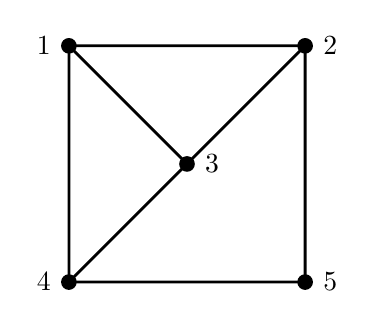
\begin{tikzpicture}[scale=1.5]
					\node [dot={180}{1}] at (0,2) {};
					\node [dot={0}{2}] at (2,2) {};
					\node [dot={0}{3}] at (1,1) {};
					\node [dot={180}{4}] at (0,0) {};
					\node [dot={0}{5}] at (2,0) {};

					\draw[line width=1pt]
						(0,0) -- (0,2) -- (2,2) -- (2,0) -- (0,0) -- (1,1) -- (2,2) -- (0,2) -- (1,1);
				\end{tikzpicture}
				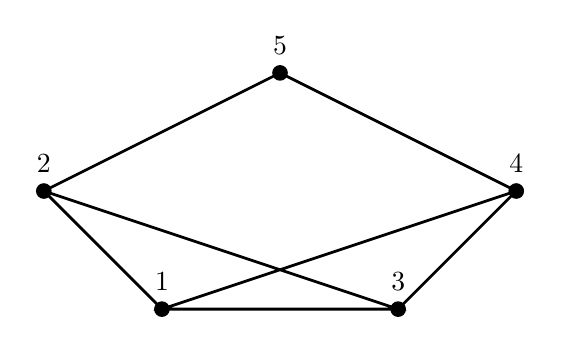
\begin{tikzpicture}[scale=1.5]
					\node [dot={90}{1}] at (1,0) {};
					\node [dot={90}{2}] at (0,1) {};
					\node [dot={90}{3}] at (3,0) {};
					\node [dot={90}{4}] at (4,1) {};
					\node [dot={90}{5}] at (2,2) {};

					\draw[line width=1pt]
						(0,1) -- (1,0) -- (3,0) -- (4,1) -- (2,2) -- (0,1) -- (3,0) -- (1,0) -- (4,1);	
				\end{tikzpicture}
			\end{center}

			These are two different illustrations that both represent $G$.
		\end{ex}
		
		\begin{defn}
			Given the following graph:
			\begin{center}
				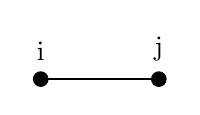
\begin{tikzpicture}[scale=1.5]
					\node [dot={90}{i}] at (0,0) {};
					\node [dot={90}{j}] at (1,0) {};

					\draw[line width=1pt]
						(0,0) -- (1,0);
				\end{tikzpicture}
			\end{center}
			If $ij \in E$, we say $i$ and $j$ are \textbf{endpoints} of $ij$. We also say that $i, j$ are \textbf{adjacent}, and that edge $ij$ is \textbf{incident} to $i$ and $j$.
			\\ \\
			The neighbours of $v \in V$ are defined as $\set{v \in V | v u \in E}$.
		\end{defn}

		\begin{ex}
			Given the following graph:
			\begin{center}
				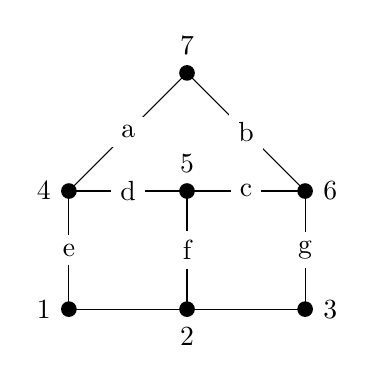
\begin{tikzpicture}[scale=1.5]
					\node [dot={180}{1}] at (0,0) {};
					\node [dot={-90}{2}] at (1,0) {};
					\node [dot={0}{3}] at (2,0) {};
					\node [dot={180}{4}] at (0,1) {};
					\node [dot={90}{5}] at (1,1) {};
					\node [dot={0}{6}] at (2,1) {};
					\node [dot={90}{7}] at (1,2) {};

					\draw (0,1) -- (1,2) node [midway,fill=white] {a};
					\draw (1,2) -- (2,1) node [midway,fill=white] {b};
					\draw (2,1) -- (1,1) node [midway,fill=white] {c};
					\draw (1,1) -- (0,1) node [midway,fill=white] {d};
					\draw (0,1) -- (0,0) node [midway,fill=white] {e};
					\draw (1,0) -- (1,1) node [midway,fill=white] {f};
					\draw (2,0) -- (2,1) node [midway,fill=white] {g};
					\draw (0,0) -- (2,0);
				\end{tikzpicture}
			\end{center}
			The endpoints of $f$ are $2$ and $5$. $1$ and $2$ are adjacent. $c, d,$ and $f$ are the edges incident to $5$. The neighbours of 2 are 1, 3, and 5.
		\end{ex}

		\begin{ex}
			If we were to represent a street map as a graph, $V$ would be the set of intersections and $E$ would be the set of streets.
		\end{ex}

		\begin{ex}
			If we were to represent a network of people, $V$ would be a set of individuals and $E$ would be the various relationships between those people (sets of friends).
		\end{ex}

		\begin{ex}
			Let $V$ be the set of binary strings of length $n$.
			\\ \\
			$uv \in E$ if $u$ and $v$ differ in exactly $k$ positions. We have $n = 3$ (since at most 3 differ) and $k = 1$. We get the following graph:

			\begin{center}
				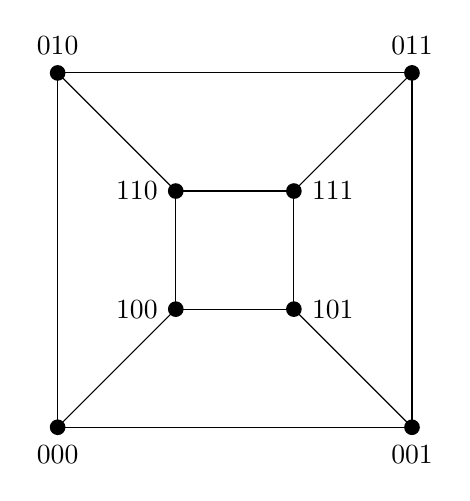
\begin{tikzpicture}[scale=1.5]
					\node [dot={-90}{000}] at (0,0) {};
					\node [dot={-90}{001}] at (3,0) {};
					\node [dot={90}{010}] at (0,3) {};
					\node [dot={90}{011}] at (3,3) {};
					\node [dot={180}{100}] at (1,1) {};
					\node [dot={0}{101}] at (2,1) {};
					\node [dot={180}{110}] at (1,2) {};
					\node [dot={0}{111}] at (2,2) {};

					\draw (0,0) -- (3,0) -- (3,3) -- (0,3) -- (0,0);
					\draw (1,1) -- (1,2) -- (2,2) -- (2,1) -- (1,1);
					\draw (0,0) -- (1,1);
					\draw (0,3) -- (1,2);
					\draw (3,0) -- (2,1);
					\draw (3,3) -- (2,2);
				\end{tikzpicture}
			\end{center}
		\end{ex}

		\begin{ex}
			If we have the following interval graph:
			\begin{center}
				\begin{tikzpicture} % scale = 1
					\draw (0,0) -- (1,0) node [midway,fill=white] {5};
					\draw (1,5) -- (3,5) node [midway,fill=white] {1};
					\draw (2,4) -- (5,4) node [midway,fill=white] {2};
					\draw (4,3) -- (7,3) node [midway,fill=white] {3};
					\draw (3,1) -- (6,1) node [midway,fill=white] {4};
					\draw[dashed] (1,0) -- (1,5);
				\end{tikzpicture}
			\end{center}

			The overlaps are the edges. We can represent the same graph as:
			\begin{center}
				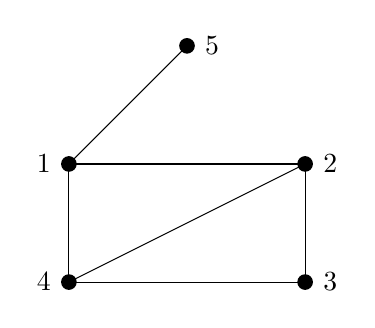
\begin{tikzpicture}[scale=1.5]
					\node [dot={180}{1}] at (0,1) {};
					\node [dot={0}{2}] at (2,1) {};
					\node [dot={0}{3}] at (2,0) {};
					\node [dot={180}{4}] at (0,0) {};
					\node [dot={0}{5}] at (1,2) {};

					\draw (0,0) -- (0,1) -- (2,1) -- (2,0) -- (0,0);
					\draw (0,0) -- (2,1);
					\draw (0,1) -- (1,2);
				\end{tikzpicture}
			\end{center}
		\end{ex}

		\subsection{Isomorphism}
			Are the following two graphs the same?
			\\ \\
			$G_1$, with vertices $V = \set{1, 2, 3, 4}$:
			\begin{center}
				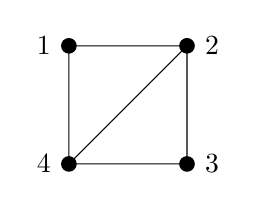
\begin{tikzpicture}[scale=1.5]
					\node [dot={180}{1}] at (0,1) {};
					\node [dot={0}{2}] at (1,1) {};
					\node [dot={0}{3}] at (1,0) {};
					\node [dot={180}{4}] at (0,0) {};

					\draw (0,0) -- (0,1) -- (1,1) -- (1,0) -- (0,0) -- (1,1);
				\end{tikzpicture}
			\end{center}

			$G_2$, with vertices $V = \set{a, b, c, d}$:
			\begin{center}
				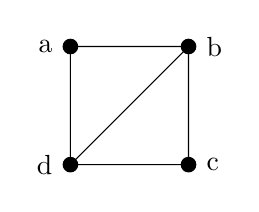
\begin{tikzpicture}[scale=1.5]
					\node [dot={180}{a}] at (0,1) {};
					\node [dot={0}{b}] at (1,1) {};
					\node [dot={0}{c}] at (1,0) {};
					\node [dot={180}{d}] at (0,0) {};

					\draw (0,0) -- (0,1) -- (1,1) -- (1,0) -- (0,0) -- (1,1);
				\end{tikzpicture}
			\end{center}

			\begin{defn}
				$G_1 = (V_1, E_1)$ and $G_2 = (V_2, E_2)$ are \textbf{isomorphic} if there exists a bijection $\phi: V_1 \to V_2$ such that $uv \in E_1 \to \phi(u) \phi(v) \in E_2$ and $uv \not \in E_1 \to \phi(u) \phi(v) \not \in E_2$.
			\end{defn}
			
			Examining the two graphs above, we have:
			\begin{align*}
				\phi(1) &= a \\
				\phi(2) &= b \\
				\phi(3) &= c \\
				\phi(4) &= d
			\end{align*}

			Pairing 1 and 3, we get $13 \in E_1 \to \phi(1)\phi(3) = ac \not \in E_2$.
			\\ \\
			Pairing 4 and 3, we get $43 \in E_1 \to \phi(4) \phi(3) = dc \in E_2$.
			\\ \\
			We must continue to consider these pairings for all edges.

			\begin{ex}
				Are the following graphs isomorphic?

				\begin{center}
					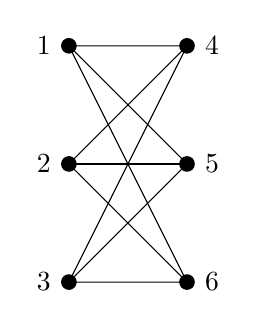
\begin{tikzpicture}[scale=1.5]
						\node [dot={180}{1}] at (0,2) {};
						\node [dot={180}{2}] at (0,1) {};
						\node [dot={180}{3}] at (0,0) {};
						\node [dot={0}{4}] at (1,2) {};
						\node [dot={0}{5}] at (1,1) {};
						\node [dot={0}{6}] at (1,0) {};

						\draw (0,0) -- (1,0) -- (0,1) -- (1,2) -- (0,2) -- (1,1) -- (0,0);
						\draw (0,0) -- (1,2);
						\draw (0,2) -- (1,0);
						\draw (0,1) -- (1,1);
					\end{tikzpicture}
					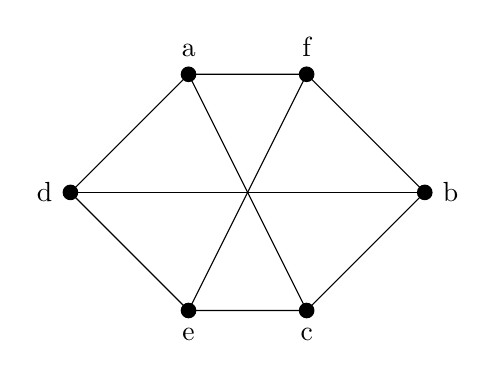
\begin{tikzpicture}[scale=1.5]
						\node [dot={90}{a}] at (1,2) {};
						\node [dot={0}{b}] at (3,1) {};
						\node [dot={-90}{c}] at (2,0) {};
						\node [dot={180}{d}] at (0,1) {};
						\node [dot={-90}{e}] at (1,0) {};
						\node [dot={90}{f}] at (2,2) {};
						
						\draw (0,1) -- (1,2) -- (2,2) -- (3,1) -- (2,0) -- (1,0) -- (0,1);
						\draw (0,1) -- (3,1);
						\draw (1,2) -- (2,0);
						\draw (1,0) -- (2,2);
					\end{tikzpicture}
				\end{center}

				Yes! There exists a bijection $\phi$:
				\begin{align*}
					1 &\to a \\
					2 &\to b \\
					3 &\to e \\
					4 &\to f \\
					5 &\to d \\
					6 &\to c
				\end{align*}

				There is no general algorithm for finding a bijection. In this case, you could see that 1, 2, and 3 have no edges and a, b, and e also have no edges.
			\end{ex}

			\begin{ex}
				Are the following graphs isomorphic?
				\begin{center}
					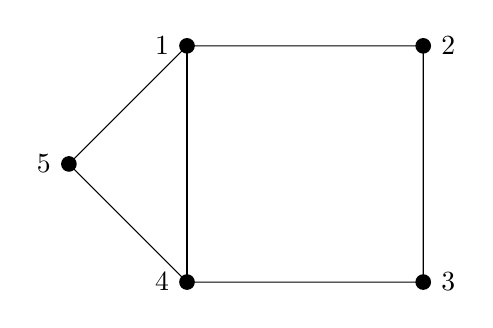
\begin{tikzpicture}[scale=1.5]
						\node [dot={180}{1}] at (1,2) {};
						\node [dot={0}{2}] at (3,2) {};
						\node [dot={0}{3}] at (3,0) {};
						\node [dot={180}{4}] at (1,0) {};
						\node [dot={180}{5}] at (0,1) {};

						\draw (0,1) -- (1,2) -- (3,2) -- (3,0) -- (1,0) -- (0,1);
						\draw (1,0) -- (1,2);
					\end{tikzpicture}
					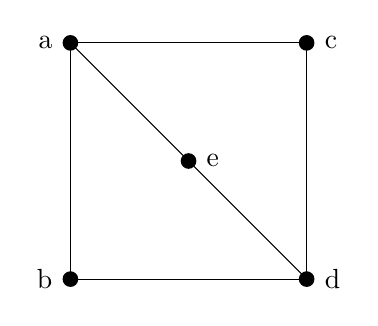
\begin{tikzpicture}[scale=1.5]
						\node [dot={180}{a}] at (0,2) {};
						\node [dot={180}{b}] at (0,0) {};
						\node [dot={0}{c}] at (2,2) {};
						\node [dot={0}{d}] at (2,0) {};
						\node [dot={0}{e}] at (1,1) {};

						\draw (0,0) -- (0,2) -- (2,2) -- (2,0) -- (0,0);
						\draw (2,0) -- (0,2);
					\end{tikzpicture}
				\end{center}
				No. 1, 4, and 5 are pairwise adjacent but there are no corresponding vertices on the second graph.
			\end{ex}

		\subsection{Degrees of Vertices}
			\begin{defn}
				The \textbf{degree} of a vertex is the number of edges incident to that vertex.
			\end{defn}

			\begin{ex}
				We have the following graph, with each vertex indicating its degree:
				\begin{center}
					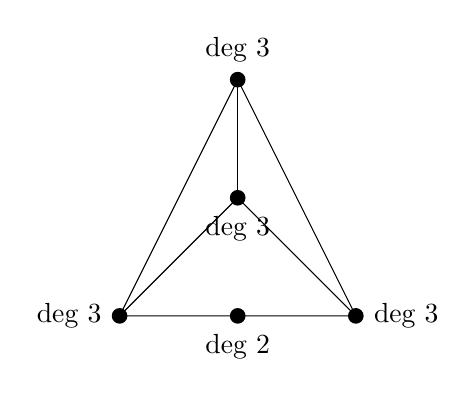
\begin{tikzpicture}[scale=1.5]
						\node [dot={180}{deg 3}] at (0,0) {};
						\node [dot={-90}{deg 2}] at (1,0) {};
						\node [dot={0}{deg 3}] at (2,0) {};
						\node [dot={-90}{deg 3}] at (1,1) {};
						\node [dot={90}{deg 3}] at (1,2) {};

						\draw (0,0) -- (2,0) -- (1,2) -- (0,0);
						\draw (0,0) -- (1,1) -- (2,0);
						\draw (1,2) -- (1,1);
					\end{tikzpicture}
				\end{center}

				Note that $|E| = 7$, and the sum of all degrees is $3 + 3 + 3 + 3 + 2 = 14$.
			\end{ex}

			\begin{theorem}
				For any graph $G = (V, E)$, $(\star) = \displaystyle \sum_{v \in V} \deg(v) = 2|E|$.
			\end{theorem}

			Also, note that there is an even number of vertices of an odd degree.
			
			\begin{ex} Given the following table:
				\begin{center}
					\begin{tabular}{c|c}
						Individuals & \# of friends among $\set{a, \ldots, i}$ \\ \hline
						a & 6 \\
						b & 3 \\
						c & 4 \\
						d & 1 \\
						e & 5 \\
						f & 3 \\
						g & 7 \\
						h & 2 \\
						i & 4
					\end{tabular}
				\end{center}
				
				There are 5 odd numbers of friends. One of them must be lying.
			\end{ex}
			
			\lecture{February 25, 2013}
			\begin{ex}
				Given the following graph:
				\begin{center}
					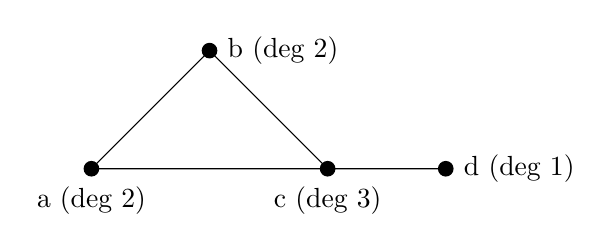
\begin{tikzpicture}[scale=1.5]
						\node [dot={-90}{a (deg 2)}] at (0, 0) {};
						\node [dot={0}{b (deg 2)}] at (1, 1) {};
						\node [dot={-90}{c (deg 3)}] at (2, 0) {};
						\node [dot={0}{d (deg 1)}] at (3, 0) {};

						\draw (0, 0) -- (1, 1) -- (2, 0) -- (3, 0) -- (0, 0);
					\end{tikzpicture}
				\end{center}

				Let's examine the degrees of $a, b, c,$ and $d$:
				\begin{align*}
					&\deg(a) + \deg(b) + \deg(c) + \deg(d) \\
					&= |\set{ab, ac}| + |\set{ab, bc}| + |\set{ac, bc, cd}| + |\set{cd}|
				\end{align*}

				Note that each edge appears exactly twice in the above equation \textendash{} once for each endpoint. This is the general idea behind the proof for the previous theorem.
			\end{ex}

			\begin{proof}
				For each edge $ab \in E$, $ab$ contributes 1 to $(\star)$ for $\deg(a)$ and $ab$ contributes 1 to $(\star)$ for $\deg(b)$.
			\end{proof}

		\subsection{Bipartite Graphs}
			\begin{defn}
				A graph $G = (V, E)$ is \textbf{bipartite} if there exists a partittion of $V$ into $V_1$ and $V_2$ such that every edge has one endpoint in $V_1$ and one endpoint in $V_2$.
			\end{defn}

			\begin{ex}
				Is the following graph bipartite?
				\begin{center}
					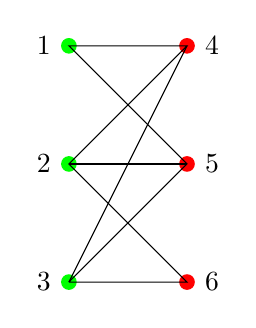
\begin{tikzpicture}[scale=1.5]
							\node [gdot={180}{1}] at (0,2) {};
							\node [gdot={180}{2}] at (0,1) {};
							\node [gdot={180}{3}] at (0,0) {};
							\node [rdot={0}{4}] at (1,2) {};
							\node [rdot={0}{5}] at (1,1) {};
							\node [rdot={0}{6}] at (1,0) {};

							\draw (0,0) -- (1,0) -- (0,1) -- (1,2) -- (0,2) -- (1,1) -- (0,0);
							\draw (0,0) -- (1,2);
							\draw (0,1) -- (1,1);
					\end{tikzpicture}
				\end{center}
				Yes, this graph is bipartite because $V_1$ could be the vertices on the left-hand side (1, 2, and 3), and $V_2$ could be the vertices on the right-hand side (4, 5, and 6).
			\end{ex}

			\begin{ex}
				Is the following graph bipartite?
				\begin{center}
					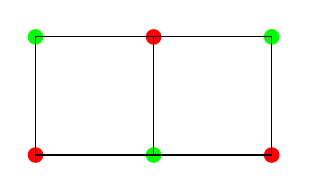
\begin{tikzpicture}[scale=1.5]
						\node [rdot={0}{}] at (0,0) {};
						\node [gdot={0}{}] at (1,0) {};
						\node [rdot={0}{}] at (2,0) {};
						\node [gdot={0}{}] at (0,1) {};
						\node [rdot={0}{}] at (1,1) {};
						\node [gdot={0}{}] at (2,1) {};

						\draw (1,0) -- (2,0) -- (2,1) -- (0,1) -- (0,0) -- (1,0) -- (1,1);
					\end{tikzpicture}
				\end{center}
				Yes, this graph is bipartite.
			\end{ex}

			Not every graph is bipartite, however.
			\begin{ex}
				Is the following graph bipartite?
				\begin{center}
					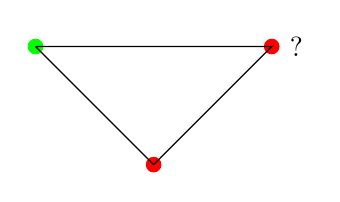
\begin{tikzpicture}[scale=1.5]
						\node [gdot={0}{}] at (0,1) {};
						\node [rdot={0}{}] at (1,0) {};
						\node [rdot={0}{?}] at (2,1) {};

						\draw (0,1) -- (1,0) -- (2,1) -- (0,1);
					\end{tikzpicture}
				\end{center}
				No, this graph is not bipartite as shown. This is the simplest graph that is not bipartite, in fact.
			\end{ex}

			\begin{ex}
				Is the following graph bipartite, and is the partitioning unique?
				\begin{center}
					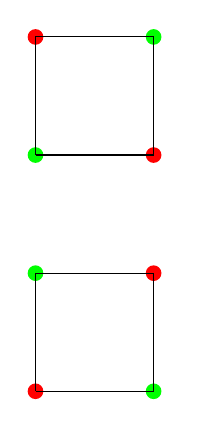
\begin{tikzpicture}[scale=1.5]
						\node [rdot={0}{}] at (0,0) {};
						\node [gdot={0}{}] at (1,0) {};
						\node [gdot={0}{}] at (0,1) {};
						\node [rdot={0}{}] at (1,1) {};

						\draw (0,0) -- (0,1) -- (1,1) -- (1,0) -- (0,0);
						
						
						\node [gdot={0}{}] at (0,2) {};
						\node [rdot={0}{}] at (1,2) {};
						\node [rdot={0}{}] at (0,3) {};
						\node [gdot={0}{}] at (1,3) {};

						\draw (0,2) -- (0,3) -- (1,3) -- (1,2) -- (0,2);
					\end{tikzpicture}
				\end{center}
				Yes, this graph is bipartite, however its partitioning is not unique. We can flip the colors (of both the squares of the graph) and still show the graph to be bipartite. So, in general, the partitioning of $V$ into $V_1$ and $V_2$ is not unique.
			\end{ex}

			The $n$-cube is the graph $G = (V, E)$ where $V$ is the set of binary strings of length $n$ and $uv$ is an edge if $u$ and $v$ differ in exactly one position. For $n = 2$, we have the following graph:
			\begin{center}
				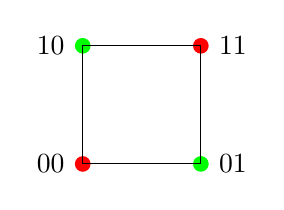
\begin{tikzpicture}[scale=1.5]
					\node [rdot={180}{00}] at (0, 0) {};
					\node [gdot={0}{01}] at (1, 0) {};
					\node [gdot={180}{10}] at (0, 1) {};
					\node [rdot={0}{11}] at (1,1) {};

					\draw (0,0) -- (0,1) -- (1,1) -- (1,0) -- (0,0);
				\end{tikzpicture}
			\end{center}

			Is the $n$-cube bipartite for any $n$? Yes!

			\begin{proof}
				Let $V_1$ be the set of strings with an even number of ones, and let $V_2$ be the set of strings with an odd number of ones. Let $uv \in E$.
				\\ \\
				Note that we can split $u$ and $v$ each into two pieces, split on the single element (character) that differs between $u$ and $v$. Corresponding pieces of $u$ and $v$ are the same.
				\\ \\
				The parity of the number of ones in $u$ is different from the number of ones in $v$, since aside from that single character difference, the parity of ones is the same between $u$ and $v$. Therefore, $u$ and $v$ are not both in $V_1$ or both in $V_2$. So, the $n$-cube is bipartite.
			\end{proof}

			\begin{proposition}
				Let $G = (V, E)$ be a bipartite graph with partition $V = V_1 \cup V_2$. Then:
				\begin{align*}
					\underbrace{\sum_{v \in V_1} \deg(v)}_{(1)} = \underbrace{\sum_{v \in V_2} \deg(v)}_{(2)} = |E|
				\end{align*}
			\end{proposition}

			Each edge has one endpoint in $V_1$ and one endpoint in $V_2$, which is why this intuitively makes sense. More formally:
			\begin{proof}
				Consider any edge $ab \in E$. Then $ab$ contributes 1 to (1) and $ab$ contributes 1 to (2).
			\end{proof}

			\begin{theorem}[Corollary]
				If $|V_1| = |V_2|$, then the average degree of vertices in $V_1$ is equal to the average degree of vertices in $V_2$.
			\end{theorem}

		\subsection{Walks, Cycles, and Paths}
			A walk is like a comet flying off track \textendash{} they're continuous lines.
			\begin{center}
				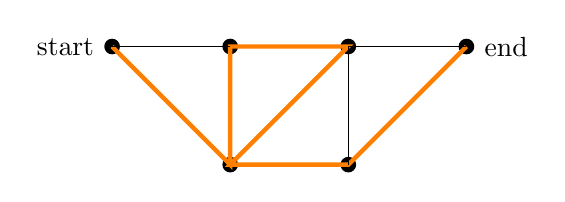
\begin{tikzpicture}[scale=1.5]
					\node [dot={0}{}] at (1, 0) {};
					\node [dot={0}{}] at (2, 0) {};
					\node [dot={180}{start}] at (0, 1) {};
					\node [dot={0}{}] at (1, 1) {};
					\node [dot={0}{}] at (2, 1) {};
					\node [dot={0}{end}] at (3, 1) {};

					\draw [orange, ultra thick] (0, 1) -- (1, 0) -- (1, 1) -- (2, 1) -- (1, 0) -- (2, 0) -- (3, 1); 
					\draw (0, 1) -- (1, 1);
					\draw (2, 1) -- (3, 1);
					\draw (2, 1) -- (2, 0);
				\end{tikzpicture}
			\end{center}

			\begin{defn}
				A \textbf{walk} $W$ on graph $G = (V, E)$ from $v_0$ to $v_n$ is a sequence $v_0 e_1 v_1 e_2 v_2 e_3 v_3 \ldots v_{n - 1} e_n v_n$ for $i = 1, \ldots, n$ where edge $e_i$ has endpoints $v_{i - 1}$ and $v_i$.
			\end{defn}

			\begin{defn}
				A \textbf{path} is a walk $W$ in which $v_0, v_1, \ldots, v_n$ are all distinct.
			\end{defn}

			\begin{defn}
				A \textbf{cycle} occurs if $v_0, v_1, \ldots, v_{n - 1}$ are distinct but $v_0 = v_n$ (the start and ending vertices are the same).
			\end{defn}

			\begin{ex}
				We have the following graph:
				\begin{center}
					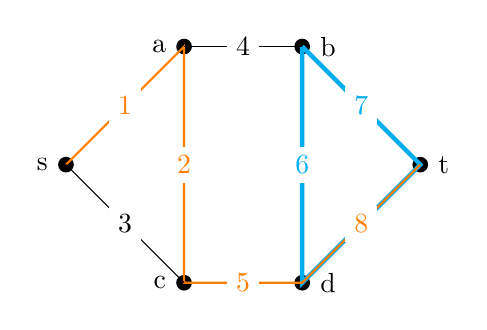
\begin{tikzpicture}[scale=1.5]
						\node [dot={-180}{c}] at (1, 0) {};
						\node [dot={0}{d}] at (2, 0) {};
						\node [dot={180}{s}] at (0, 1) {};
						\node [dot={-180}{a}] at (1, 2) {};
						\node [dot={0}{b}] at (2, 2) {};
						\node [dot={0}{t}] at (3, 1) {};

						\draw [cyan, ultra thick] (2, 2) -- (3, 1) node [midway,fill=white] {7} -- (2, 0) -- (2, 2) node [midway,fill=white] {6};
						\draw [orange, thick] (0, 1) -- (1, 2) node [midway,fill=white] {1} -- (1, 0) node [midway,fill=white] {2} -- (2, 0) node [midway,fill=white] {5} -- (3, 1) node [midway,fill=white] {8};
						\draw (0, 1) -- (1, 0) node [midway,fill=white] {3};
						\draw (1, 2) -- (2, 2) node [midway,fill=white] {4};
					\end{tikzpicture}
				\end{center}
				
				In this graph, we've visualized a path $P$ (in orange) and a cycle $C$ (in blue). We can express $P$ as $P = s1a2c5d8t$ and we can express $C$ similarly as $C = b7t8d6b$.
			\end{ex}
			
			\begin{proposition}
				Let $G = (V, E)$ be a graph, and $x, y \in V$ where $x \ne y$. If there exists a walk from $x$ to $y$, then there also exists a path from $x$ to $y$.
			\end{proposition}
			
			To find the path from a walk, when you reach a vertex that is equal to another, you ignore that cycle.

			\lecture{February 27, 2013}
			\begin{ex}
				Let's say you have the following graph:
				\begin{center}
					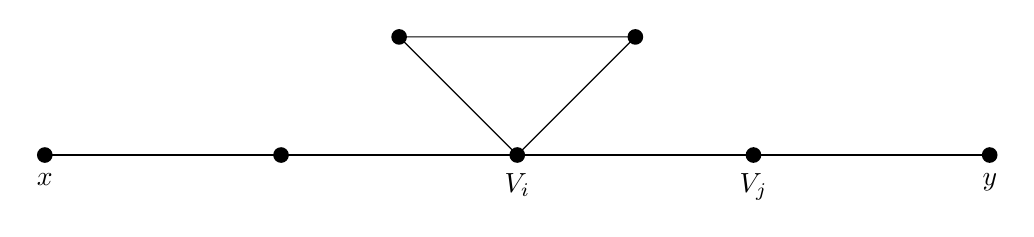
\begin{tikzpicture}[scale=1.5]
						\node [dot={-90}{$x$}] at (0,0) {};
						\node [dot={0}{}] at (2,0) {};
						\node [dot={-90}{$V_i$}] at (4,0) {};
						\node [dot={-90}{$V_j$}] at (6,0) {};
						\node [dot={-90}{$y$}] at (8,0) {};
						\node [dot={0}{}] at (3,1) {};
						\node [dot={0}{}] at (5,1) {};

						\draw (0,0) -- (8,0);
						\draw (4,0) -- (5,1) -- (3,1) -- (4,0);
					\end{tikzpicture}
				\end{center}

				Heading from $x$ to $y$, while going through the nodes in the triangle in the middle, is a walk. However, if we were to skip visiting the $V_i$-th node entirely, we would have a path.
			\end{ex}

			\begin{proof}
				Among all walks from $x$ to $y$, pick a walk $W$ with as few edges as possible. We would pick:
				\begin{align*}
					W = V_0e_1V_1e_2V_2 \ldots e_nV_n \text{ where } V_0 = x_1 \text{ and } V_n = y
				\end{align*}

				We need to show that $V_0, V_1, \ldots, V_n$ are all distinct. Suppose for a contradiction that there exists $V_i = V_j$ for some $i < j$. That would mean:
				\begin{align*}
					W &= V_0 \ldots e_i \underbrace{V_ie_{i + 1} \ldots e_j}_{\text{cut off}} V_je_{j + 1} \ldots V_n \\
					\implies W' &= V_0 \ldots e_iV_je_{j + 1} \ldots V_n
				\end{align*}

				$W'$ is still a walk from $x$ to $y$. But $W'$ has fewer edges than $W$, which is a contradiction.
			\end{proof}

			\begin{theorem}[Corollary]
				If there exists a path from $x$ to $y$ and there exists a path from $y$ to $z$, then there exists a path from $x$ to $z$.
			\end{theorem}

			This corollary is not as trivial to show as you might initially think. You can't just join the two paths, because the two paths may share some vertices. 
			\begin{proof}
				The path from $x$ to $y$ followed by the path from $y$ to $z$ is a walk from $x$ to $z$ (\emph{not} a path). By the previous result, there exists a path from $x$ to $z$.
			\end{proof}

			Does every graph have a cycle?
			\begin{center}
				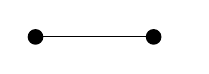
\begin{tikzpicture}[scale=1.5]
					\node [dot={0}{}] at (0,0) {};
					\node [dot={0}{}] at (1,0) {};

					\draw (0,0) -- (1,0);
				\end{tikzpicture}
			\end{center}

			This graph does clearly not have a cycle, but it's not a terribly interesting graph. This more complicated graph also does not have a cycle:
			\begin{center}
				\begin{tikzpicture}[scale=1.5]
					\node [dot={0}{}] at (0,0) {};
					\node [dot={0}{}] at (1,0) {};
					\node [dot={0}{}] at (2,0) {};
					\node [dot={0}{}] at (1,1) {};

					\node [dot={0}{}] at (3,2) {};

					\node [dot={0}{}] at (0,4) {};
					\node [dot={0}{}] at (1,4) {};
					\node [dot={0}{}] at (2,4) {};
					\node [dot={0}{}] at (2,3) {};

					\node [dot={0}{}] at (6,1) {};
					\node [dot={0}{}] at (6,2) {};
					\node [dot={0}{}] at (5,3) {};
					\node [dot={0}{}] at (7,3) {};
					\node [dot={0}{}] at (8,2) {};

					\draw (1,1) -- (0,0);
					\draw (1,1) -- (1,0);
					\draw (1,1) -- (2,0);

					\draw (3,2) -- (1,1);
					\draw (3,2) -- (2,3);

					\draw (2,3) -- (0,4);
					\draw (2,3) -- (1,4);
					\draw (2,3) -- (2,4);

					\draw (3,2) -- (8,2);
					\draw (6,2) -- (6,1);
					\draw (6,2) -- (5,3);
					\draw (6,2) -- (7,3);
				\end{tikzpicture}
			\end{center}

			But what if every vertex has degree at least 2? In that case, it is not possible to create a graph that does \emph{not} have a cycle. In order for each vertex to have degree of at least 2, it must loop back somewhere.
			\begin{proposition}
				Let $G = (V, E)$. If for all $v \in V$, $\deg(v) \ge 2$, then $G$ has a cycle.
			\end{proposition}

			\begin{proof}
				Among all paths, pcik a path $P$ with as many edges as possible. We have:
				\begin{align*}
					P = V_0e_1V_1e_2 \ldots e_nV_n
				\end{align*}

				Since $\deg(V_n) \ge 2$, there exists $V_nw \ne e_n$. Since $P$ is the longest path, $w = V_i$ for some $i \in \set{0, \ldots, n - 2}$. Then we have the cycle $C$:
				\begin{align*}
					C &= V_ie_iV_{i + 1} \ldots e_nV_ne_{n + 1}V_i
				\end{align*}
			\end{proof}

			Note that it doesn't necessarily have to loop back to the ``first'' vertex because you may have a graph like this:
			\begin{center}
				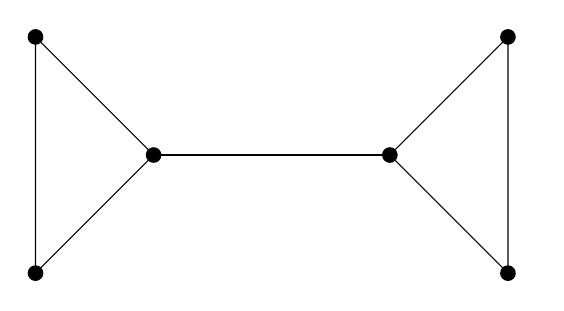
\begin{tikzpicture}[scale=1.5]
					\node [dot={0}{}] at (0,0) {};
					\node [dot={0}{}] at (1,1) {};
					\node [dot={0}{}] at (0,2) {};
					\node [dot={0}{}] at (3,1) {};
					\node [dot={0}{}] at (4,0) {};
					\node [dot={0}{}] at (4,2) {};

					\draw (0,0) -- (1,1) -- (0,2) -- (0,0);
					\draw (3,1) -- (4,0) -- (4,2) -- (3,1);
					\draw (1,1) -- (3,1);
				\end{tikzpicture}
			\end{center}

		\subsubsection{Hamiltonian Cycles}
			\begin{defn}
				A cycle is \textbf{Hamiltonian} if every vertex is in the cycle.
			\end{defn}

			You can think of a Hamiltonian cycle in terms of a graph of cities, where you have a person who wants to visit all the cities once and then return to their initial city.

			\begin{ex}
				Here's an example of a Hamiltonian cycle:
				\begin{center}
					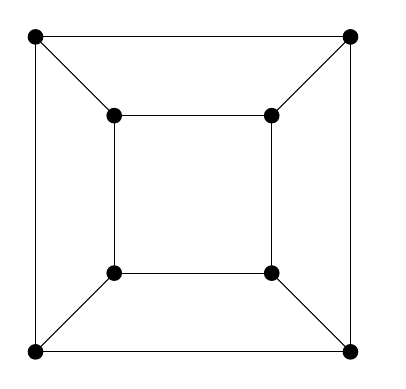
\begin{tikzpicture}%[scale=1.5]
						\node [dot={0}{}] at (0,0) {};
						\node [dot={0}{}] at (4,0) {};
						\node [dot={0}{}] at (0,4) {};
						\node [dot={0}{}] at (4,4) {};

						\node [dot={0}{}] at (1,1) {};
						\node [dot={0}{}] at (3,1) {};
						\node [dot={0}{}] at (1,3) {};
						\node [dot={0}{}] at (3,3) {};

						\draw (0,0) -- (4,0) -- (4,4) -- (0,4) -- (0,0);
						\draw (1,1) -- (1,3) -- (3,3) -- (3,1) -- (1,1);
						\draw (0,0) -- (1,1);
						\draw (4,4) -- (3,3);
						\draw (0,4) -- (1,3);
						\draw (4,0) -- (3,1);
					\end{tikzpicture}
				\end{center}
			\end{ex}

			Do we always have a Hamiltonian cycle? No.
			\begin{ex}
				Here's an example of a graph without a Hamiltonian cycle.
				\begin{center}
					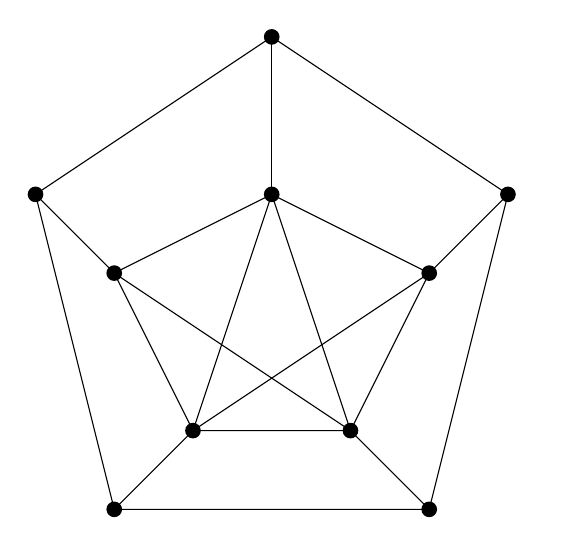
\begin{tikzpicture}%[scale=1.5]
						\node [dot={0}{}] at (0,4) {};
						\node [dot={0}{}] at (1,0) {};
						\node [dot={0}{}] at (5,0) {};
						\node [dot={0}{}] at (2,1) {};
						\node [dot={0}{}] at (4,1) {};
						\node [dot={0}{}] at (1,3) {};
						\node [dot={0}{}] at (5,3) {};
						\node [dot={0}{}] at (3,4) {};
						\node [dot={0}{}] at (6,4) {};
						\node [dot={0}{}] at (3,6) {};

						\draw (0,4) -- (1,0) -- (5,0) -- (6,4) -- (3,6) -- (0,4);
						\draw (0,4) -- (1,3) -- (2,1) -- (4,1) -- (5,3) -- (3,4) -- (1,3);
						\draw (1,0) -- (2,1);
						\draw (5,0) -- (4,1);
						\draw (5,3) -- (6,4);
						\draw (3,4) -- (3,6);
						\draw (2,1) -- (5,3);
						\draw (1,3) -- (4,1) -- (3,4) -- (2,1);
					\end{tikzpicture}
				\end{center}
			\end{ex}

			\begin{proposition}
				Let $G = (V, E)$. If for all $v \in V$, $\deg(v) \ge \frac{|V|}{2}$, then there exists a Hamiltonian cycle.
			\end{proposition}

		\subsection{Disjoint Paths} \lecture{March 1, 2013}
			\begin{ex}
				Given the following graph:
				\begin{center}
					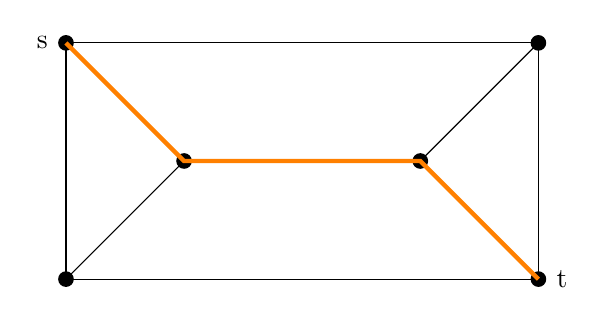
\begin{tikzpicture}[scale=1.5]
						\node [dot={0}{}] at (0,0) {};
						\node [dot={0}{t}] at (4,0) {};
						\node [dot={180}{s}] at (0,2) {};
						\node [dot={0}{}] at (4,2) {};
						\node [dot={0}{}] at (1,1) {};
						\node [dot={0}{}] at (3,1) {};

						\draw (0,0) -- (4,0) -- (4,2) -- (0,2) -- (0,0);
						\draw (0,0) -- (1,1) -- (0,2);
						\draw (4,0) -- (3,1) -- (4,2);
						\draw (1,1) -- (3,1);
						\draw [orange, ultra thick] (0,2) -- (1,1) -- (3,1) -- (4,0);
					\end{tikzpicture}
				\end{center}

				Is there a path from $s$ to $t$? Yes, there are several.
			\end{ex}

			\begin{ex}
				Given the following graph:
				\begin{center}
					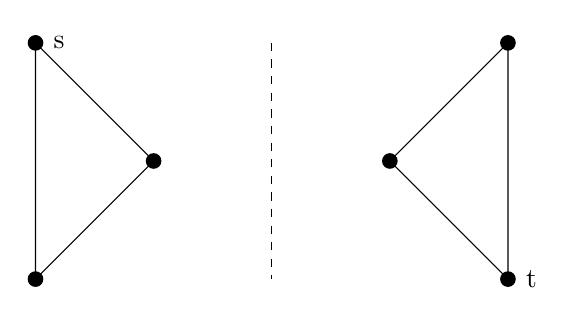
\begin{tikzpicture}[scale=1.5]
						\node [dot={0}{}] at (0,0) {};
						\node [dot={0}{t}] at (4,0) {};
						\node [dot={0}{}] at (1,1) {};
						\node [dot={0}{}] at (3,1) {};
						\node [dot={0}{s}] at (0,2) {};
						\node [dot={0}{}] at (4,2) {};
						
						\draw (0,0) -- (1,1) -- (0,2) -- (0,0);
						\draw (4,0) -- (4,2) -- (3,1) -- (4,0);
						\draw [dashed] (2,2) -- (2,0);
					\end{tikzpicture}
				\end{center}

				Is there a path from $s$ to $t$? No. The two sets of vertices have no edges between them.
			\end{ex}

			\begin{defn}
				A pair of paths is \textbf{edge disjoint} if the paths do not share an edge.
			\end{defn}

			\begin{ex}
				Given the following graph:
				\begin{center}
					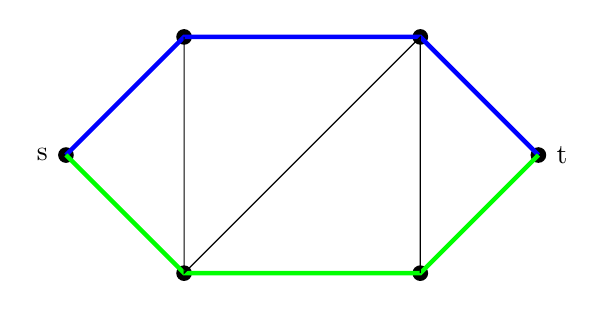
\begin{tikzpicture}[scale=1.5]
						\node [dot={180}{s}] at (0,1) {};
						\node [dot={0}{}] at (1,0) {};
						\node [dot={0}{}] at (1,2) {};
						\node [dot={0}{}] at (3,0) {};
						\node [dot={0}{}] at (3,2) {};
						\node [dot={0}{t}] at (4,1) {};

						\draw [blue, ultra thick] (0,1) -- (1,2) -- (3,2) -- (4,1);
						\draw [green, ultra thick] (0,1) -- (1,0) -- (3,0) -- (4,1);
						\draw (1,0) -- (1,2) -- (1,0) -- (3,2) -- (3,0);
					\end{tikzpicture}
				\end{center}

				Are there two edge disjoint paths from $s$ to $t$? Yes. There is no edge that is both blue and green, so the two paths are disjoint.
			\end{ex}

			\begin{ex}
				Given the following graph:
				\begin{center}
					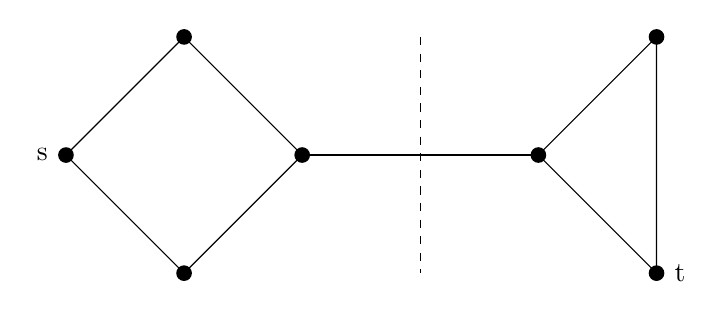
\begin{tikzpicture}[scale=1.5]
						\node [dot={180}{s}] at (0,1) {};
						\node [dot={0}{}] at (1,0) {};
						\node [dot={0}{}] at (1,2) {};
						\node [dot={0}{}] at (2,1) {};
						\node [dot={0}{}] at (4,1) {};
						\node [dot={0}{t}] at (5,0) {};
						\node [dot={0}{}] at (5,2) {};

						\draw (0,1) -- (1,0) -- (2,1) -- (1,2) -- (0,1);
						\draw (4,1) -- (5,0) -- (5,2) -- (4,1);
						\draw (2,1) -- (4,1);
						\draw [dashed] (3,2) -- (3,0);
					\end{tikzpicture}
				\end{center}

				Are there two edge disjoint paths from $s$ to $t$? No. For the same reason as the two examples above, the center edge must be used in all paths because it is the only edge that connects two otherwise disjoint sets of vertices.
			\end{ex}
			
			\begin{ex}
				Given the following graph:
				\begin{center}
					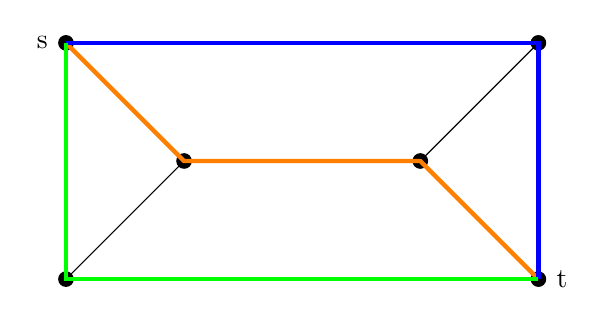
\begin{tikzpicture}[scale=1.5]
						\node [dot={0}{}] at (0,0) {};
						\node [dot={0}{t}] at (4,0) {};
						\node [dot={180}{s}] at (0,2) {};
						\node [dot={0}{}] at (4,2) {};
						\node [dot={0}{}] at (1,1) {};
						\node [dot={0}{}] at (3,1) {};

						\draw (0,0) -- (4,0) -- (4,2) -- (0,2) -- (0,0);
						\draw (0,0) -- (1,1) -- (0,2);
						\draw (4,0) -- (3,1) -- (4,2);
						\draw (1,1) -- (3,1);
						\draw [orange, ultra thick] (0,2) -- (1,1) -- (3,1) -- (4,0);
						\draw [blue, ultra thick] (0,2) -- (4,2) -- (4,0);
						\draw [green, ultra thick] (0,2) -- (0,0) -- (4,0);
					\end{tikzpicture}
				\end{center}
				
				Are there \underline{three} edge disjoint paths from $s$ to $t$? Yes, as shown.
				\label{ex:threedisjointpaths}
			\end{ex}
			
			\begin{ex}
				Given the following graph:
				\begin{center}
					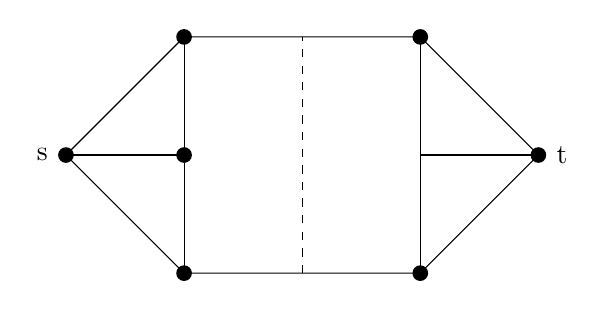
\begin{tikzpicture}[scale=1.5]
						\node [dot={180}{s}] at (0,1) {};
						\node [dot={0}{}] at (1,0) {};
						\node [dot={0}{}] at (1,1) {};
						\node [dot={0}{}] at (1,2) {};
						\node [dot={0}{}] at (3,0) {};
						\node [dot={0}{}] at (3,2) {};
						\node [dot={0}{t}] at (4,1) {};
						
						\draw (0,1) -- (1,2) -- (3,2) -- (4,1) -- (3,0) -- (1,0) -- (0,1);
						\draw (0,1) -- (1,1);
						\draw (1,0) -- (1,2);
						\draw (4,1) -- (3,1);
						\draw (3,0) -- (3,2);
						\draw [dashed] (2,0) -- (2,2);
;					\end{tikzpicture}
				\end{center}
				
				This is an example of a graph with two disjoint paths but not three. There are just two edges connecting two otherwise disjoint sets of vertices.
			\end{ex}
			
			Let $G = (V,E)$, and let $S \subseteq V, S \ne \emptyset, S \ne V$ (we pick a proper subset of vertices). We define:
			\begin{align*}
				\delta(S) := \set{uv \in E | u \in S, v \not \in S}
			\end{align*}
			
			Informally, $\delta(S)$ is the set of edges between $V$ and $V \backslash S$.
			
			\begin{ex}
				Given the following graph:
				\begin{center}
					\begin{tikzpicture}[scale=1.5]
						\node [dot={180}{s}] at (0,1) {};
						\node [dot={-90}{b}] at (1,0) {};
						\node [dot={90}{a}] at (1,2) {};
						\node [dot={90}{c}] at (2,1) {};
						\node [dot={90}{d}] at (4,1) {};
						\node [dot={0}{t}] at (5,0) {};
						\node [dot={0}{}] at (5,2) {};

						\draw (0,1) -- (1,0) -- (2,1) -- (1,2) -- (0,1);
						\draw (4,1) -- (5,0) -- (5,2) -- (4,1);
						\draw (2,1) -- (4,1);
						\draw [dashed] (3,2) -- (3,0);
					\end{tikzpicture}
				\end{center}
				
				If $S = \set{s, a, b, c}$, we get $\delta(S) = \set{cd}$.
			\end{ex}
			
			\begin{ex}
				Given the following graph:
				\begin{center}
					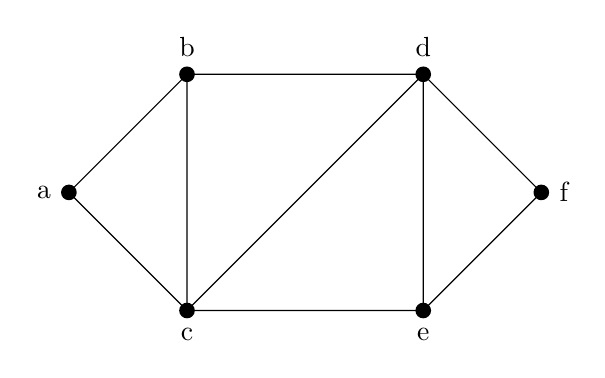
\begin{tikzpicture}[scale=1.5]
						\node [dot={180}{a}] at (0,1) {};
						\node [dot={-90}{c}] at (1,0) {};
						\node [dot={90}{b}] at (1,2) {};
						\node [dot={-90}{e}] at (3,0) {};
						\node [dot={90}{d}] at (3,2) {};
						\node [dot={0}{f}] at (4,1) {};

						\draw (0,1) -- (1,2) -- (3,2) -- (4,1);
						\draw (0,1) -- (1,0) -- (3,0) -- (4,1);
						\draw (1,0) -- (1,2) -- (1,0) -- (3,2) -- (3,0);
					\end{tikzpicture}
				\end{center}
				
				If $S = \set{b, e}$, we get $\delta(S) = \set{ab, bc, bd, ec, ed, ef}$.
			\end{ex}
			
			\begin{defn}
				$\delta(S)$ (which is a set of edges) is the \textbf{cut induced} by $S$.
			\end{defn}
			
			We say it's a cut because if we removed (cut) those edges, we would get two sets of edges with no edges connecting the two sets, so the graph would fall apart.
			
			\begin{defn}
				Let $s, t \in V (s \ne t)$. If $s \in S$ and $t \not \in S$, then $\delta(S)$ is an \textbf{$\mathbf{st}$-cut}.
			\end{defn}
			
			In \ref{ex:threedisjointpaths}, we have a $st$-cut of size 2, which is why we cannot find three disjoint paths from $s$ to $t$.

			\subsubsection{Menger's Theorem}
				\begin{theorem}
					Let $G = (V, E)$ be a graph, and $s, t \in V (s \ne t)$. If there exists edge disjoint paths $P_1, P_2, \ldots, P_k$ from $s$ to $t$, then for all $st$-cuts of $\delta(S)$, $|\delta(S)| \ge k$.
					\\ \\
					Equivalently, if you have an $st$-cut of size less than $k$, you cannot find $k$ disjoint paths from $s$ to $t$.
				\end{theorem}
			
				\begin{proof}
					Let $\delta(S)$ be an $st$-cut ($s \in S, t \not \in S$). Let $i \in \set{1, \ldots, k}$. Follow $P_i$ from $s$ to $t$. Let $v_i$ be the last vertex in $S$ of $P_i$, and let $w_i$ be the first vertex \emph{not} in $S$ of $P_i$. Then $e_i = v_i w_i$ is an edge of $P_i$ and $e_i \in \delta(S)$. This implies $\set{e_1, e_2, \ldots, e_k} \subseteq \delta(S)$.
					\\ \\
					Since $P_1, P_2, \ldots, P_k$ are edge disjoint, $e_1, e_2, \ldots, e_k$ are all different. This implies that $\delta(S)| \ge k$. Since $\delta(S)$ was an arbitrary cut, we have shown that all $st$-cuts have at least $k$ edges.
				\end{proof}
			
				The converse is also true, which is known as Menger's Theorem.
			
				\begin{theorem}[Menger's Theorem]
					Let $G = (V, E)$ be a graph, and $s, t \in V (s \ne t)$. If for all $st$-cuts $\delta(S)$, $|\delta(S)| \ge k$, then there exist edge disjoint paths $P_1, \ldots, P_k$ from $s$ to $t$.
				\end{theorem}
			
				\begin{proof}
					The proof of Menger's Theorem is by performing induction on $|E| + |V|$. The base case is where you have two vertices and no edge between them, as seen here:
					\begin{center}
						\begin{tikzpicture}[scale=1.5]
							\node [dot={180}{s}] at (0,1) {};
							\node [dot={0}{t}] at (2,1) {};
						
							\draw [dashed] (1,2) -- (1,0);
						\end{tikzpicture}
					\end{center}
				
					There are then two cases:
					\begin{enumerate}
						\item There exists $e_1$ and no $st$-cut that contains $e_1$ has exactly $k$ edges.
						\item Say, $k = 3$, for instance. Divide the graph in two, and shrink the vertices from half the graph into a single consolidated vertex. Then apply the same logic for the other half of the graph. By induction, we can find three paths on both of the smaller graphs. We want to combine these two smaller paths, which we can do by connecting the corresponding paths of the two sub-graphs.
					\end{enumerate}
				\end{proof}

				\begin{theorem}[Corollary] \lecture{March 4, 2013}
					There exists a path from $s$ to $t$ (1) if and only if for all $s \subseteq V, s \in S, \delta(S) \ne \emptyset$ (2).
				\end{theorem}

				\begin{proof}
					Let us prove that (2) implies (1).
					\\ \\
					Let $U = \set{s} \cup \set{v | \exists \text{ a path from } s \text{ to } v}$. If $t \in U$, we're done. 
					\\ \\
					Let's assume $t \not \in U$. By (2), there exists $ab \in \delta(v)$, say $a \in U, b \not \in U$. That is, we have at least one edge leaving $U$.
					\\ \\
					Informally, we know we have a path from $s$ to $a$. We can take that path and add the edge $ab$ to get us a path from $s$ to $b$. However, then $b$ should be in $U$ as well, because there exists a path from $s$ to $b$.
					\\ \\
					Formally, since $a \in U$, there exists a path $P_a$ from $s$ to $a$. Construct a path $P_b$ by adding edge $ab$ at the end of $P_a$. This implies that $b \in U$, which is a contradiction.
				\end{proof}

			\subsubsection{Connectedness, Subgraphs, and Components}
				\begin{defn}
					A graph is \textbf{connected} if there exists a path between any pair of vertices. If a graph is not connected, it is \textbf{disconnected}.
				\end{defn}
				
				\begin{ex}
					This graph is disconnected:
					\begin{center}
						\begin{tikzpicture}[scale=1.5]
							\node [dot={-90}{s}] at (0,0) {};
							\node [dot={-90}{t}] at (2,0) {};
						\end{tikzpicture}
					\end{center}
				\end{ex}

				\begin{ex}
					This graph (considered as a whole) is disconnected:
					\begin{center}
						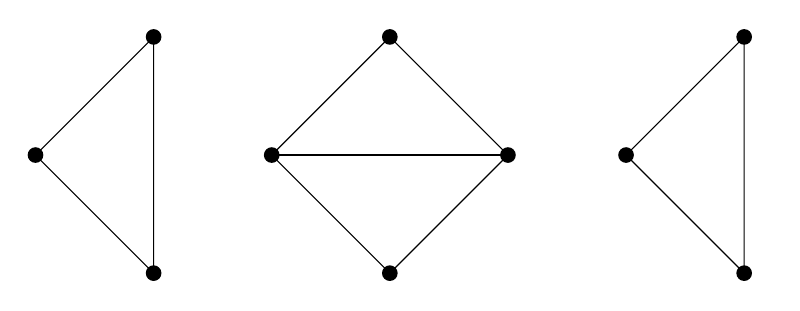
\begin{tikzpicture}[scale=1.5]
							\node [dot={0}{}] at (0,1) {};
							\node [dot={0}{}] at (1,0) {};
							\node [dot={0}{}] at (1,2) {};
							\draw (0,1) -- (1,0) -- (1,2) -- (0,1);

							\node [dot={0}{}] at (2,1) {};
							\node [dot={0}{}] at (3,0) {};
							\node [dot={0}{}] at (3,2) {};
							\node [dot={0}{}] at (4,1) {};
							\draw (2,1) -- (3,0) -- (4,1) -- (3,2) -- (2,1);
							\draw (2,1) -- (4,1);

							\node [dot={0}{}] at (5,1) {};
							\node [dot={0}{}] at (6,0) {};
							\node [dot={0}{}] at (6,2) {};
							\draw (5,1) -- (6,0) -- (6,2) -- (5,1);
						\end{tikzpicture}
					\end{center}
				\end{ex}

				This corollary follows immediately from our characterization of $st$-cuts:
				\begin{theorem}[Corollary]
					$G$ is connected (1) if and only if for all $X \subseteq V, X \ne \emptyset, X \ne V, \delta(X) \ne \emptyset$ (2).
				\end{theorem}

				\begin{defn}
					$H = (V_H, E_H)$ is a \textbf{subgraph} of $G = (V_G, E_G)$ if $V_H \subseteq V_G$ and $E_H \subseteq E_G$.
				\end{defn}

				\begin{ex}
					The highlighted portion of this graph is a subgraph:
					\begin{center}
						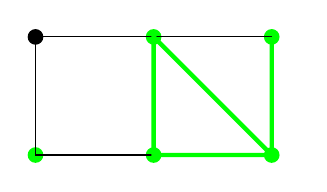
\begin{tikzpicture}[scale=1.5]
							\node [gdot={0}{}] at (0,0) {};
							\node [dot={0}{}] at (0,1) {};
							\node [gdot={0}{}] at (1,0) {};
							\node [gdot={0}{}] at (1,1) {};
							\node [gdot={0}{}] at (2,0) {};
							\node [gdot={0}{}] at (2,1) {};

							\draw (2,1) -- (0,1) -- (0,0) -- (1,0);
							\draw [green, ultra thick] (2,1) -- (2,0) -- (1,1) -- (1,0) -- (2,0);
						\end{tikzpicture}
					\end{center}
				\end{ex}

				Note that in order to keep an edge in a subgraph, we must keep both of its vertices. When we discard a vertex, we must discard all edges that have that vertex as an endpoint.

				\begin{defn}
					A \textbf{component} of a graph is a maximal connected subgraph of $G$. That is, a component is the connected subgraph of $G$ that has the same number of edges as vertices.
				\end{defn}

				\begin{ex}
					Given the following graph $G$ (considered as a whole):
					\begin{center}
						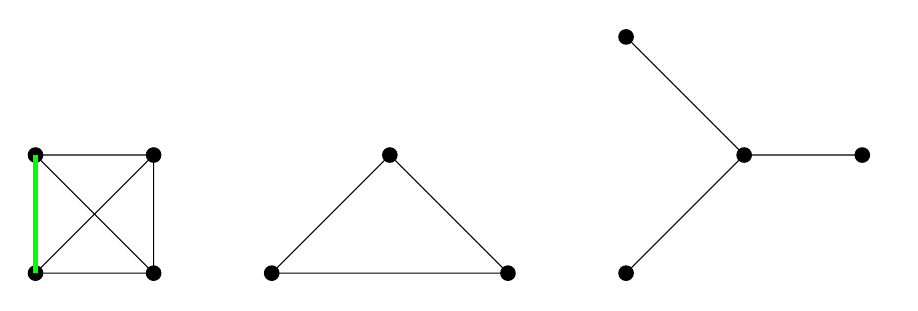
\begin{tikzpicture}[scale=1.5]
							\node [dot={0}{}] at (0,0) {};
							\node [dot={0}{}] at (0,1) {};
							\node [dot={0}{}] at (1,0) {};
							\node [dot={0}{}] at (1,1) {};
							\draw (0,0) -- (0,1) -- (1,1) -- (1,0) -- (0,0) -- (1,1);
							\draw (0,1) -- (1,0);
							\draw [green, ultra thick] (0,1) -- (0,0);

							\node [dot={0}{}] at (2,0) {};
							\node [dot={0}{}] at (3,1) {};
							\node [dot={0}{}] at (4,0) {};
							\draw (2,0) -- (3,1) -- (4,0) -- (2,0);

							\node [dot={0}{}] at (5,0) {};
							\node [dot={0}{}] at (5,2) {};
							\node [dot={0}{}] at (6,1) {};
							\node [dot={0}{}] at (7,1) {};
							\draw (5,0) -- (6,1) -- (7,1);
							\draw (5,2) -- (6,1);
						\end{tikzpicture}
					\end{center}

					Each of these three obviously-disjoint subgraphs are components. The highlighted portion is not itself a component (as expected), because it is not a \underline{maximal} subgraph.
				\end{ex}

				\begin{theorem}[Remark]
					$G$ is connected if and only if $G$ has a single component.
				\end{theorem}

			\subsubsection{Equivalence Relations}
				\begin{defn}
					$\mathbf{\sim}$ is an \textbf{equivalence relation} for $S$ (an infinite set) if all of the following hold:
					\begin{enumerate}
						\item For all $a \in S$, $a \sim a$ (reflexivity).
						\item For all $a, b \in S$, $a \sim b \implies b \sim a$ (symmetry).
						\item For all $a, b, c \in S$, if $a \sim b$ and $b \sim c$, then $a \sim c$ (transitivity).
					\end{enumerate}
				\end{defn}

				\begin{ex}
					Let $S$ be the set of all integers. Pick some integer $m \ge 1$. A sample equivalence relation would be $a \sim b$ if $a - b$ is a multiple of $m$.
				\end{ex}

				You can always partition your set $S$ into \textbf{equivalence classes}.
				
				\begin{ex}
					Let $G = (V, E)$ be a graph. Given $a, b \in V$, $a \sim b$ if $a = b$ or there exists a path from $a$ to $b$. We propose that $\sim$ is an equivalence relation, and we want to prove it.
					\begin{proof}
						We have to prove all three parts of the definition of equivalence relations.
						\\ \\
						(1) is true by definition.
						\\ \\
						(2) is true because if there exists a path from $a$ to $b$, then there exists a path from $b$ to $a$.
						\\ \\
						(3) is true because if there exists a path from $a$ to $b$ and there exists a path from $b$ to $c$, then there exists a path from $a$ to $c$ (by theorem).
						\\ \\
						Therefore, we have shown that $\sim$ is indeed an equivalence relation.
					\end{proof}
				\end{ex}

				\textbf{Question}: what do the equivalence classes correspond to? Any two vertices with one component should have a path \emph{and} one vertex from a component and one vertex from another component should \emph{not} have a path between them. The equivalence classes correspond to the vertices of each of the components of $G$.
				\\ \\
				\textbf{Exercise}: look at set $S$ (the set of all possible graphs). We propose that $G \sim H$ if $G$ is isomorphic to $H$. Prove that $\sim$ is an equivalence relation.
				\\ \\
				\textbf{Remark}: it's useful to think of paths and cycles as sets of edges. Reflexivity makes a lot more sense under this interpretation, for instance. Cycles become a set of edges of a connected subgraph where every vertex has degree two. Paths are edges of a connected subgraph where two vertices have degree one and every other vertex degree two.
				
			\subsubsection{Bridges}
				\begin{defn}
					Let $G = (V, E)$ be a graph, and $e \in E$. Then, $G \backslash e$ is the graph obtained from $G$ by deleting edge $e$. We say $e$ is a \textbf{bridge} of $G$ if $G \backslash e$ has more components than $G$.
				\end{defn}

				\begin{ex}
					Given the following graph:
					\begin{center}
						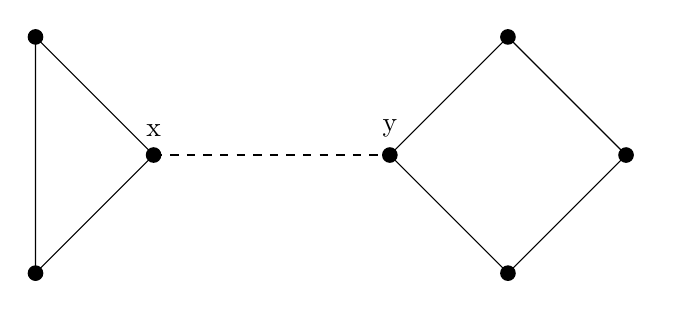
\begin{tikzpicture}[scale=1.5]
							\node [dot={0}{}] at (0,0) {};
							\node [dot={0}{}] at (0,2) {};
							\node [dot={90}{x}] at (1,1) {};
							\node [dot={90}{y}] at (3,1) {};
							\node [dot={0}{}] at (4,0) {};
							\node [dot={0}{}] at (4,2) {};
							\node [dot={0}{}] at (5,1) {};

							\draw (0,0) -- (0,2) -- (1,1) -- (0,0);
							\draw (3,1) -- (4,0) -- (5,1) -- (4,2) -- (3,1);
							\draw [dashed] (1,1) -- (3,1);
						\end{tikzpicture}
					\end{center}

					The edge $xy$ is a bridge, because if it was removed the number of components will increase from one to two. If this edge was removed, $x$ and $y$ would be in different components. This can be proven by transitivity.
				\end{ex}

				
				\begin{proposition} \lecture{March 6, 2013}
					If $e = xy$ is a bridge of $G$, then $x$ and $y$ are in distinct components of $G \backslash e$.
				\end{proposition}

				\begin{proof}
					There exists $ab$ such that $a$ and $b$ are in the same component of $G$, but $a$ and $b$ are in distinct components of $G \backslash e$. This implies that there exists a path $P$ in $G$ between $a$ and $b$ that uses $e$.
					\\ \\
					Suppose for a contradiction that $x$ and $y$ are in the same component of $G \backslash e$. We know:
					\begin{itemize}
						\item $a$ and $x$ are in the same component of $G \backslash e$ (because of $P$).
						\item $b$ and $y$ are in the same component of $G \backslash e$ (because of $P$).
					\end{itemize}

					By transitivity, $a$ and $b$ must be in the same component, which is a contradiction.
				\end{proof}

				\begin{proposition}
					Let $G = (V, E)$ be a connected graph, and let $e$ be a bridge of $G$. Then $G \backslash e$ has exactly two components.
				\end{proposition}

				\begin{proof}
					Let $X$ be the vertices in the component of $G \backslash e$ that contains $x$. Let $Y = V \backslash X$. We need to show that any two vertices in $Y$ are connected by a path in $G \backslash e$.
					\\ \\
					Let $a, b \in Y$. Since $G$ is connected, there exists a path $P_a$ between $a$ and $x$ in $G$, and there exists a path $P_b$ between $b$ and $x$ in $G$. Moreover, $P_a$ and $P_b$ both use the edge $e$. This implies:
					\begin{itemize}
						\item $a$ and $y$ are in the same component of $G \backslash e$.
						\item $b$ and $y$ are in the same component of $G \backslash e$.
					\end{itemize}

					By transitivity, $a$ and $b$ are in the same component of $G \backslash e$.
				\end{proof}

				Note that we didn't just prove that there exists a path from $a$ and $b$ to $y$ because we wanted to ensure that the path did not use the edge $e$.

				\begin{proposition}
					Let $G = (V, E)$ be a graph, and $e \in E$. $e$ is \emph{not} a bridge (1) if and only if $e$ is in a cycle (2).
				\end{proposition}
				
				In fact, this is the only reason you wouldn't have a bridge.

				\begin{proof}
					Assume $e = xy$. We'll start by proving that (1) implies (2).
					\\ \\
					The fact that $e = xy$ is not a bridge implies that there exists a path $P$ between $x$ and $y$ in $G \backslash e$. Then, $P \cup \set{e}$ is a cycle.
					\\ \\
					Now, we'll prove (2) implies (1).
					\\ \\
					If $e$ is in a cycle $C$, then $G \backslash e$ is a path between $x$ and $y$. This implies that $e$ is not a bridge, otherwise $x$ and $y$ are in distinct components of $G \backslash e$, as proven earlier.
				\end{proof}

				\begin{proposition}
					Let $G = (V, E)$ be a graph. Let $a, b \in V$ (where $a \ne b$). Suppose there exists paths $P_1, P_2$ between $a$ and $b$ where $P_1$ and $P_2$ are distinct. Then $G$ has a cycle.
				\end{proposition}

				We want to show that there is a cycle that uses the edge $e$. So, we need to show that there exists a path from $x$ to $y$ that does not use the edge $e$.

				\begin{proof}
					Since $P_1$ is distinct from $P_2$, there exists an edge $e = xy$ in $P_2$ that is not in $P_1$. After possibly interchanging $a$ and $b$, we know:
					\begin{itemize}
						\item $a$ and $x$ are in the same component of $G \backslash e$ (because of $P_2$).
						\item $y$ and $b$ are in the same component of $G \backslash e$ (because of $P_2$).
						\item $a$ and $b$ are in the same component of $G \backslash e$ (because of $P_1$).
					\end{itemize}

					Using those facts, by transitivity we know there exists a path $P$ between $x$ and $y$ in $G \backslash e$. Then $P \cup \set{e}$ is a cycle.
				\end{proof}
		\subsection{Trees}
			\begin{defn}
				A graph $G$ is a \textbf{tree} if $G$ is connected and $G$ has no cycle.
			\end{defn}

			\begin{ex}
				This graph is not a tree because it contains cycles:
				\begin{center}
					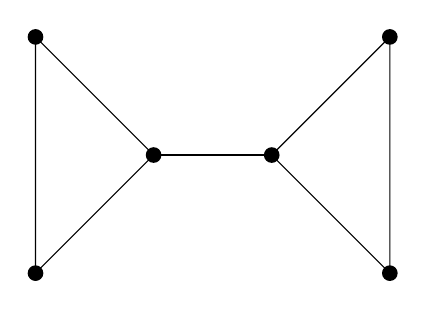
\begin{tikzpicture}[scale=1.5]
						\node [dot={0}{}] at (0,0) {};
						\node [dot={0}{}] at (0,2) {};
						\node [dot={0}{}] at (1,1) {};
						\node [dot={0}{}] at (2,1) {};
						\node [dot={0}{}] at (3,0) {};
						\node [dot={0}{}] at (3,2) {};

						\draw (0,0) -- (0,2) -- (1,1) -- (0,0);
						\draw (3,0) -- (2,1) -- (3,2) -- (3,0);
						\draw (1,1) -- (2,1);
					\end{tikzpicture}
				\end{center}
			\end{ex}

			\begin{ex}
				This graph (considered as a whole) is not a tree because it is disconnected:
				\begin{center}
					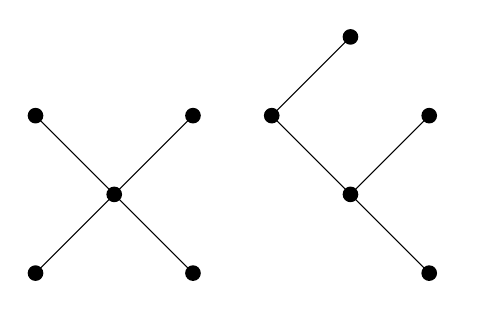
\begin{tikzpicture}%[scale=1.5]
						\node [dot={0}{}] at (0,0) {};
						\node [dot={0}{}] at (0,2) {};
						\node [dot={0}{}] at (1,1) {};
						\node [dot={0}{}] at (2,0) {};
						\node [dot={0}{}] at (2,2) {};
						\draw (0,0) -- (1,1) -- (0,2);
						\draw (2,0) -- (1,1) -- (2,2);

						\node [dot={0}{}] at (3,2) {};
						\node [dot={0}{}] at (4,1) {};
						\node [dot={0}{}] at (4,3) {};
						\node [dot={0}{}] at (5,2) {};
						\node [dot={0}{}] at (5,0) {};
						\draw (3,2) -- (4,1) -- (5,2);
						\draw (3,2) -- (4,3);
						\draw (4,1) -- (5,0);
					\end{tikzpicture}
				\end{center}
			\end{ex}

			\begin{ex}
				This graph is a tree because it is connected and has no cycles:
				\begin{center}
					\begin{tikzpicture}[scale=1.5]
						\node [dot={0}{}] at (4,0) {};
						\node [dot={0}{}] at (2,1) {};
						\node [dot={0}{}] at (3,2) {};
						\node [dot={0}{}] at (1,2) {};
						\node [dot={0}{}] at (0,3) {};
						\node [dot={0}{}] at (1,3) {};
						\node [dot={0}{}] at (2,3) {};
						\node [dot={0}{}] at (6,1) {};
						\node [dot={0}{}] at (5,2) {};
						\node [dot={0}{}] at (7,2) {};
						\node [dot={0}{}] at (5,3) {};
						\node [dot={0}{}] at (7,3) {};

						\draw (4,0) -- (2,1) -- (0,3);
						\draw (1,2) -- (1,3);
						\draw (1,2) -- (2,3);
						\draw (2,1) -- (3,2);

						\draw (4,0) -- (6,1) -- (7,2);
						\draw (6,1) -- (6,2) -- (7,3);
						\draw (6,2) -- (5,3);
						\draw (6,1) -- (5,2);
					\end{tikzpicture}
				\end{center}
			\end{ex}

			\begin{ex}
				This graph is also a tree:
				\begin{center}
					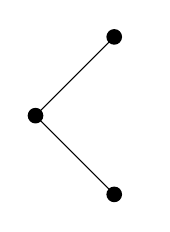
\begin{tikzpicture}%[scale=1.5]
						\node [dot={0}{}] at (0,1) {};
						\node [dot={0}{}] at (1,0) {};
						\node [dot={0}{}] at (1,2) {};

						\draw (1,0) -- (0,1) -- (1,2);
					\end{tikzpicture}
				\end{center}
			\end{ex}

			\begin{ex}
				This is the simplest graph that is a tree:
				\begin{center}
					
\begin{tikzpicture}
						\node [dot={0}{}] at (0,0) {};
					\end{tikzpicture}
				\end{center}

				Keep this graph (just one vertex with no edges) in mind when doing inductive proofs involving trees.
			\end{ex}

			\begin{proposition}
				Let $G = (V, E)$ be a tree. For all $a, b \in V$, there exists a unique path between $a$ and $b$.
			\end{proposition}

			Why is this? Simple: trees have no cycles.
			
			\begin{proposition} \lecture{March 8, 2013}
				If $G$ is a tree, then:
				\begin{enumerate}
					\item Any two distinct vertices are joined by a unique path.
					\item Every edge is a bridge.
				\end{enumerate}
			\end{proposition}

			\begin{proof}
				We will prove each part of this proposition in turn.
				\begin{enumerate}
					\item Since the tree is connected, there exists at least one path. If there exists two distinct paths between a pair of vertices, then there exists a cycle, which is a contradiction.
					\item If an edge is not a bridge, then that edge is in a cycle, which is a contradiction.
				\end{enumerate}
			\end{proof}

			\begin{proposition}
				Let $H = (V, E)$ be a tree. Let $a, b \in V$ be two distinct vertices with no edge between them. Let $G$ be the graph obtained from $H$ by adding the edge $ab$. Then $G$ has exactly one cycle.
			\end{proposition}

			\begin{ex}
				Let's add the edge $ab$ to the following tree:
				\begin{center}
					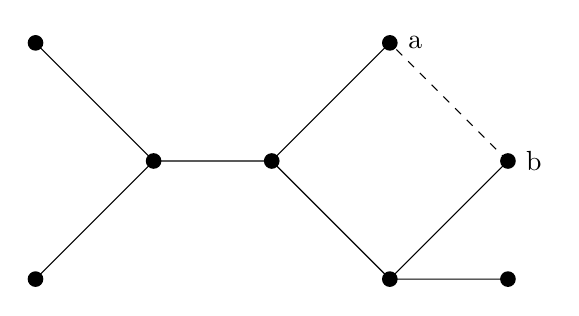
\begin{tikzpicture}[scale=1.5]
						\node [dot={0}{}] at (0,0) {};
						\node [dot={0}{}] at (0,2) {};
						\node [dot={0}{}] at (1,1) {};
						\node [dot={0}{}] at (2,1) {};
						\node [dot={0}{a}] at (3,2) {};
						\node [dot={0}{}] at (3,0) {};
						\node [dot={0}{b}] at (4,1) {};
						\node [dot={0}{}] at (4,0) {};

						\draw (0,0) -- (1,1) -- (0,2);
						\draw (1,1) -- (2,1) -- (3,2);
						\draw (2,1) -- (3,0) -- (4,0);
						\draw (3,0) -- (4,1);
						\draw [dashed] (4,1) -- (3,2);
					\end{tikzpicture}
				\end{center}

				According to the previous proposition, this graph should contain only one cycle.
			\end{ex}

			\begin{proof}
				$C$ is a cycle of $G$ if and only if $C \backslash \set{e}$ is a path of $H$ between $a$ and $b$. We know that there exists a unique such path.
			\end{proof}

			You could add an edge to create a cycle, then remove \emph{any} edge from within the cycle to get a different tree. This technique could be used by shipping companies to find the most optimal cost-efficient route to ship a package.

			\begin{defn}
				Let $G' = (V', E')$ be a subgraph of $G = (V, E)$. $G'$ is a \textbf{spanning subgraph} if $V' = V$.
			\end{defn}

			\begin{ex}
				This is not a spanning subgraph because one vertex in $V$ is not included in $V'$:
				\begin{center}
					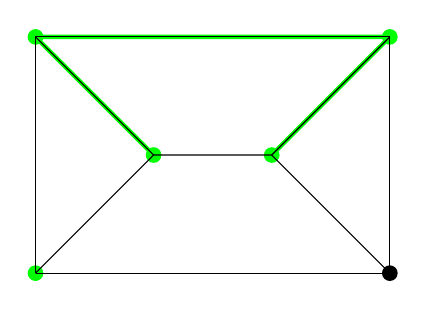
\begin{tikzpicture}[scale=1.5]
						\node [gdot={0}{}] at (0,0) {};
						\node [gdot={0}{}] at (0,2) {};
						\node [gdot={0}{}] at (1,1) {};
						\node [gdot={0}{}] at (2,1) {};
						\node [gdot={0}{}] at (3,2) {};
						\node [dot={0}{}] at (3,0) {};
						
						\draw [green, ultra thick] (1,1) -- (0,2) -- (3,2) -- (2,1);
						\draw (0,0) -- (3,0) -- (3,2) -- (0,2) -- (0,0);
						\draw (0,0) -- (1,1) -- (0,2);
						\draw (1,1) -- (2,1) -- (3,2);
						\draw (2,1) -- (3,0);
					\end{tikzpicture}
				\end{center}
			\end{ex}

			\begin{ex}
				This is a spanning subgraph because $V' = V$:
				\begin{center}
					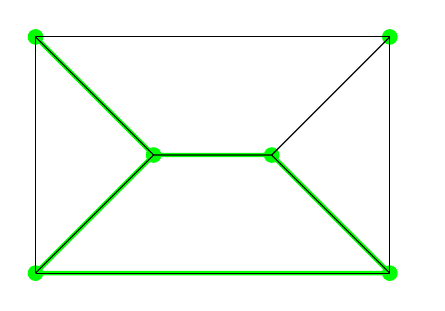
\begin{tikzpicture}[scale=1.5]
						\node [gdot={0}{}] at (0,0) {};
						\node [gdot={0}{}] at (0,2) {};
						\node [gdot={0}{}] at (1,1) {};
						\node [gdot={0}{}] at (2,1) {};
						\node [gdot={0}{}] at (3,2) {};
						\node [gdot={0}{}] at (3,0) {};
						
						\draw [green, ultra thick] (0,2) -- (1,1) -- (0,0) -- (3,0) -- (2,1) -- (1,1);
						\draw (0,0) -- (3,0) -- (3,2) -- (0,2) -- (0,0);
						\draw (0,0) -- (1,1) -- (0,2);
						\draw (1,1) -- (2,1) -- (3,2);
						\draw (2,1) -- (3,0);
					\end{tikzpicture}
				\end{center}
			\end{ex}

			\begin{proposition}
				Let $G = (V, E)$ be a graph. $G$ is connected (1) if and only if $G$ contains a spanning tree (2).
			\end{proposition}

			\begin{ex}
				This is a graph that is connected. Its spanning tree is highlighted:
				\begin{center}
					\begin{tikzpicture}[scale=1.5]
						\node [gdot={0}{}] at (0,0) {};
						\node [gdot={0}{}] at (0,2) {};
						\node [gdot={0}{}] at (1,1) {};
						\node [gdot={0}{}] at (3,0) {};
						\node [gdot={0}{}] at (3,2) {};

						\draw [green, ultra thick] (0,0) -- (1,1) -- (0,2);
						\draw [green, ultra thick] (3,0) -- (1,1) -- (3,2);
						\draw (0,0) -- (3,0) -- (3,2) -- (0,2) -- (0,0) -- (1,1) -- (0,2);
						\draw (3,0) -- (1,1) -- (3,2);
					\end{tikzpicture}
				\end{center}
			\end{ex}

			\begin{ex}
				We have to specify that $G$ contains a \emph{spanning} tree because otherwise we would say the following graph (considered as a whole) is connected (which it is not):
				\begin{center}
					\begin{tikzpicture}[scale=1.5]
						\node [dot={0}{}] at (0,0) {};
						\node [dot={0}{}] at (0,2) {};
						\node [dot={0}{}] at (1,1) {};
						\draw (0,0) -- (1,1) -- (0,2) -- (0,0);

						\node [dot={0}{}] at (2,0) {};
						\node [dot={0}{}] at (2,2) {};
						\draw (2,0) -- (2,2);
					\end{tikzpicture}
				\end{center}
			\end{ex}

			\begin{proof}
				We'll first prove that (2) implies (1). For all $a, b \in V$ ($a \ne b$), there exists a path between $a$ and $b$ in the spanning tree. But this is also a path of $G$.
				\\ \\
				Now, we'll prove that (1) implies (2). Among all spanning subgraphs of $G$ that are connected, pick one with as few edges as possible. Call that subgraph $T$.
				\\ \\
				We claim that $T$ is a tree. We need to verify that.
				\begin{itemize}
					\item $T$ is clearly connected.
					\item $T$ does not contain a cycle, otherwise any edge on that cycle could be removed while still keeping the graph connected (edges in cycles are not bridges).
				\end{itemize}
			\end{proof}

			Let $n$ be the number of vertices in a graph $G$. If $n = 1$, we must have zero edges. If $n = 2$, we must have one edge. If $n = 3$, we must have two edges. If $n = 4$, we must have three edges. If $n = 5$, we must have four edges. Let's generalize this.

			\begin{proposition}
				In a tree, the number of edges is equal to the number of vertices minus one.
			\end{proposition}

			In order to prove this with induction, we want to start with the larger graph to see how we built it up. We can't do induction the normal way initially with graphs in general because of how graphs can be constructed (there are multiple graphs we can form a graph where $n = 5$ from a graph where $n = 4$).

			\begin{proof}
				Let $G = (V, E)$ be a tree. By induction on $|V|$:
				\\ \\
				\textbf{Base case}: $|V| = 1, |E| = 0$.
				\\ \\
				Assume $|V| \ge 2$. We claim that there exists a vertex $v$ of degree 1 (otherwise there exists a cycle). So, $v$ is adjacent to a unique vertex $w$.
				\\ \\
				Let $G' = (V', E')$ be the graph obtained from $G$ by deleting the edge $wv$ and the vertex $v$. Note that $G'$ is a tree because the degree of $v$ is one in $G$.
				\\ \\
				By induction, $|E'| = |V'| - 1$. We know that $|E| = |E'| + 1$ and $|V| = |V'| + 1$, which gives us $|E| = |V| - 1$, as required.
			\end{proof}

			If you're ever asked to determine a result involving the number of edges in a tree, you'll likely use this proposition.

		\subsection{More on Bipartite Graphs}
			\begin{proposition}
				If a graph has a cycle with an odd number of edges, then it is not bipartite.
			\end{proposition}

			\lecture{March 11, 2013}
			This graph is bipartite:
			\begin{center}
				\begin{tikzpicture}[scale=1.5]
					\node [gdot={0}{}] at (0,0) {};
					\node [rdot={0}{}] at (1,0) {};
					\node [gdot={0}{}] at (2,0) {};
					\node [rdot={0}{}] at (0,1) {};
					\node [gdot={0}{}] at (1,1) {};
					\node [rdot={0}{}] at (2,1) {};

					\draw (0,0) -- (2,0) -- (2,1) -- (0,1) -- (0,0);
					\draw (1,1) -- (1,0);
				\end{tikzpicture}
			\end{center}

			But this one is not:
			\begin{center}
				\begin{tikzpicture}%[scale=1.5]
					\node [rdot={0}{}] at (1,0) {};
					\node [gdot={0}{}] at (3,0) {};
					\node [rdot={0}{}] at (0,1) {};
					\node [rdot={0}{}] at (4,1) {};
					\node [gdot={0}{}] at (2,2) {};

					\draw (1,0) -- (3,0) -- (4,1) -- (2,2) -- (0,1);
					\draw (0,1) -- (1,0) node [midway,fill=white] {$\ddot\frown$};
				\end{tikzpicture}
			\end{center}

			\begin{proof}
				Let $C = V_1, V_2, \ldots, V_{2n}$, where $V_1 = V_{2n}$.
				\\ \\
				Suppose there exists partition $X, Y$. We may assume $V_1 \in X, V_2 \in Y, V_3 \in X, \ldots$. This implies that $V_{2n} \in Y$ since all vertices with even indices are members of $Y$. 
				\\ \\
				Notice that $V_1 \in X$ and $V_{2n} \in Y$, but $V_1 = V_{2n}$. This is a contradiction.
			\end{proof}

			We want to show that this is the \emph{only} reason why a graph would not be bipartite.
			\begin{proposition}
				A graph is bipartite if and only if all its components are bipartite.
			\end{proposition}
			
			The proof of this proposition is left as an exercise.
			\begin{proposition}
				Trees are bipartite.
			\end{proposition}

			For example, this tree is bipartite:
			\begin{center}
				\begin{tikzpicture}%[scale=1.5]
					\node [gdot={0}{}] at (0,0) {};
					\node [rdot={0}{}] at (1,1) {};
					\node [gdot={0}{}] at (0,2) {};

					\node [gdot={0}{}] at (3,1) {};
					\node [rdot={0}{}] at (4,0) {};
					\node [rdot={0}{}] at (4,2) {};
					\node [gdot={0}{}] at (5,1) {};
					\node [gdot={0}{}] at (5,3) {};

					\draw (0,0) -- (1,1) -- (0,2);
					\draw (1,1) -- (3,1) -- (4,0);
					\draw (3,1) -- (4,2) -- (5,1);
					\draw (4,2) -- (5,3);
				\end{tikzpicture}
			\end{center}

			There are a couple of different proof techniques we could use to prove this proposition.
			\begin{enumerate}
				\item We could call one vertex $V_1$ and then define even/odd vertices based on whether their distance from $V_1$ is even or odd (since there exists a unique path from $V_1$ to any other vertex in a tree). 
				\item More simplistically, we could build up the partition recursively. As we add an additional edge, each endpoint of the edge should be in the opposite partition.
			\end{enumerate}

			We'll use approach (2) to prove this proposition.
			\begin{proof}
				Let $T = (V, E)$. We're going to perform induction on $|V|$.
				\\ \\
				Base case: $|V| = 1$, i.e. $|V| = \set{v}$, set $X = \set{v}, Y = \emptyset$.
				\\ \\
				Otherwise, $|V| \ge 2$. Since $T$ is a tree, there exists vertex $u$ of degree 1. Then, $u$ is adjacent to a unique vertex $w$.
				\\ \\
				Let $T'$ be obtained by removing $uv$ and $u$. Note that $T'$ is still a tree. We can verify that fact by seeing that we're certainly not adding any cycles (not possible when removing an edge) and since $u$ has degree 1, the tree remains connected.
				\\ \\
				By induction, there exists a partition $X', Y'$ of the vertices of $T'$ such that every edge of $T'$ has one end in $X'$ and one end in $Y'$.
				\\ \\
				If $w \in X'$ then $X = X'$ and $Y = Y' \cup \set{u}$. Otherwise (if $w \in Y'$), $X = X' \cup \set{u}$ and $Y = Y'$.
			\end{proof}

			\begin{theorem}
				$G = (V, E)$ is bipartite (1) if and only if $G$ has no odd cycles (2).
			\end{theorem}

			\begin{proof}
				We proved NOT (2) implies NOT (1), which is equivalent to proving (1) implies (2). Now, we'll prove the other direction: (2) implies (1).
				\\ \\
				Due to the proposition from earlier, we may assume $G$ is connected, without loss of generality. This implies that $G$ contains a spanning tree $T = (V, E')$.
				\\ \\
				We showed that $T$ is bipartite. Let $X, Y$ be the corresponding partition of $V$.
				\\ \\
				\underline{Claim}: for all $ab \in E$, $a \in X$ and $b \in Y$, or vice versa ($a \in Y, b \in X$). We may assume $ab \in E \backslash E'$.
				\\ \\
				Let $P$ be the unique path in $T$ between $a$ and $b$. Suppose $a, b \in X$ (or $a, b \in Y$). Then $P$ has an even number of edges.
				\\ \\
				This implies that the cycle $P \cup \set{ab}$ is an odd cycle, which is a contradiction.
			\end{proof}
			
			\subsubsection{Graph Coloring}
				\begin{problem}
					Assign colors to vertices such that every edge has endpoints of different colors. The goal is to use as few colors as possible.
				\end{problem}

				What graphs can be colored with two colors? Easy: bipartite graphs.
				\\ \\
				What graphs can be colored with three colors? No clue. There's no efficient or reliable way of coloring an arbitrary graph with any constant (even very large) number of colors.

		\subsection{Planar Graphs}
			We will allow:
			\begin{itemize}
				\item Loops:
					\begin{center}
						\begin{tikzpicture}[scale=1.5]
							\node [dot={0}{},draw] {} edge [in=30,out=90,loop] ();
						\end{tikzpicture}
					\end{center}
				\item Parallel edges:
					\begin{center}
						\begin{tikzpicture}[scale=1.5]
							\node [dot={0}{}] at (0,0) {};
							\node [dot={0}{}] at (2,0) {};

							\draw (0,0) to[out=90,in=90] (2,0);
							\draw (0,0) to [out=-90,in=-90] (2,0);
						\end{tikzpicture}
					\end{center}
			\end{itemize}

			\begin{defn}
				A \textbf{planar embedding} is a drawing of a graph where no two edges cross.
			\end{defn}

			\begin{ex}
				This is not a planar embedding of a graph $G$ because two edges cross:
				\begin{center}
					\begin{tikzpicture}[scale=2]
						\node [dot={0}{}] at (0,0) {};
						\node [dot={0}{}] at (1,0) {};
						\node [dot={0}{}] at (0,1) {};
						\node [dot={0}{}] at (1,1) {};

						\draw (0,1) -- (1,1) node [midway,fill=white] {1};
						\draw (0,0) -- (0,1) node [midway,fill=white] {2};
						\draw (0,0) -- (1,0) node [midway,fill=white] {3};
						\draw (1,0) -- (0,1) node [near start,fill=white] {4};
						\draw (0,0) -- (1,1) node [near end,fill=white] {5};
					\end{tikzpicture}
				\end{center}

				This is a planar embedding for the same graph:
				\begin{center}
					\begin{tikzpicture}[scale=2]
						\node [dot={0}{}] at (0,0) {};
						\node [dot={0}{}] at (1,0) {};
						\node [dot={0}{}] at (0,1) {};
						\node [dot={0}{}] at (1,1) {};

						\draw (0,1) -- (1,1) node [midway,fill=white] {1};
						\draw (0,0) -- (0,1) node [midway,fill=white] {2};
						\draw (0,0) -- (1,0) node [midway,fill=white] {3};
						\draw (1,0) -- (0,1) node [midway,fill=white] {4};

						\draw (0,0) to[in=190,out=-30] (1.5,-0.5) to[in=0,out=80] (1,1);
					\end{tikzpicture}
				\end{center}
			\end{ex}

			\underline{Observation}: the same graph can have many different planar embeddings. We'll formally define ``different'' a bit later.
			
			\begin{ex}
				Here are two planar embeddings of the same graph $G_1$:
				\begin{center}
					\begin{tikzpicture}[scale=2]
						\node [dot={0}{}] at (0,0) {};
						\node [dot={0}{}] at (2,0) {};
						\node [dot={0}{}] at (3,0) {};
						\node [dot={0}{}] at (0,1) {};
						\node [dot={0}{}] at (2,1) {};
						\node [dot={0}{}] at (3,1) {};

						\draw (0,1) -- (2,1) node [midway,fill=white] {1};
						\draw (0,0) -- (0,1) node [midway,fill=white] {2};
						\draw (0,0) -- (2,0) node [midway,fill=white] {3};
						\draw (2,0) -- (2,1) node [midway,fill=white] {4};
						\draw (2,1) -- (3,1) node [midway,fill=white] {5};
						\draw (3,0) -- (3,1) node [midway,fill=white] {6};
						\draw (2,0) -- (3,0) node [midway,fill=white] {7};
					\end{tikzpicture}
					\begin{tikzpicture}[scale=2]
						\node [dot={0}{}] at (0,0) {};
						\node [dot={0}{}] at (2,0.25) {};
						\node [dot={0}{}] at (3,0) {};
						\node [dot={0}{}] at (0,1) {};
						\node [dot={0}{}] at (2,0.75) {};
						\node [dot={0}{}] at (3,1) {};

						\draw (0,1) -- (3,1) node [midway,fill=white] {1};
						\draw (0,0) -- (0,1) node [midway,fill=white] {2};
						\draw (0,0) -- (3,0) node [midway,fill=white] {3};
						\draw (3,0) -- (3,1) node [midway,fill=white] {4};
						\draw (3,1) -- (2,0.75) node [midway,fill=white] {5};
						\draw (2,0.75) -- (2,0.25) node [midway,fill=white] {6};
						\draw (3,0) -- (2,0.25) node [midway,fill=white] {7};
					\end{tikzpicture}
				\end{center}
			\end{ex}

			\begin{ex}
				Here are two planar embeddings of the same graph $G_2$ that look similar, except the edges are labelled differently:
				\begin{center}
					\begin{tikzpicture}[scale=2]
						\node [dot={0}{}] at (0,0) {};
						\node [dot={0}{}] at (1,1) {};
						\node [dot={0}{}] at (2,0) {};
						\node [dot={0}{}] at (1,2) {};

						\draw (0,0) -- (1,2) node [midway,fill=white] {1};
						\draw (1,2) -- (2,0) node [midway,fill=white] {2};
						\draw (0,0) -- (2,0) node [midway,fill=white] {3};
						\draw (0,0) -- (1,1) node [midway,fill=white] {4};
						\draw (1,1) -- (1,2) node [midway,fill=white] {5};
						\draw (1,1) -- (2,0) node [midway,fill=white] {6};
					\end{tikzpicture}
					\begin{tikzpicture}[scale=2]
						\node [dot={0}{}] at (0,0) {};
						\node [dot={0}{}] at (1,1) {};
						\node [dot={0}{}] at (2,0) {};
						\node [dot={0}{}] at (1,2) {};

						\draw (0,0) -- (1,2) node [midway,fill=white] {1};
						\draw (1,2) -- (2,0) node [midway,fill=white] {5};
						\draw (0,0) -- (2,0) node [midway,fill=white] {4};
						\draw (0,0) -- (1,1) node [midway,fill=white] {3};
						\draw (1,1) -- (1,2) node [midway,fill=white] {2};
						\draw (1,1) -- (2,0) node [midway,fill=white] {6};
					\end{tikzpicture}
				\end{center}
			\end{ex}

			\begin{defn}
				A graph is \textbf{planar} if there exists a planar embedding.
			\end{defn}

			\begin{ex}
				This graph is planar:
				\begin{center}
					\begin{tikzpicture}[scale=2]
						\node [dot={0}{}] at (0,0) {};
						\node [dot={0}{}] at (2,0) {};
						\node [dot={0}{}] at (0,1) {};
						\node [dot={0}{}] at (2,1) {};
						\node [dot={0}{}] at (1,2) {};

						\draw (0,0) -- (2,0) -- (2,1) -- (1,2) -- (0,1) -- (0,0) -- (2,1);
						\draw (0,1) -- (2,0);
						\draw (0,0) -- (1,2);
						\draw (0,0) -- (2,1);
					\end{tikzpicture}
				\end{center}

				It is possible to find a planar embedding for this graph.
			\end{ex}

			\begin{ex}
				These two graphs are not planar:
				\begin{center}
					\begin{tikzpicture}
						\node [dot={0}{}] at (1,0) {};
						\node [dot={0}{}] at (3,0) {};
						\node [dot={0}{}] at (0,3) {};
						\node [dot={0}{}] at (4,3) {};
						\node [dot={0}{}] at (2,4) {};
						
						\draw (1,0) -- (3,0) -- (4,3) -- (2,4) -- (0,3) -- (1,0);
						\draw (1,0) -- (2,4) -- (3,0) -- (0,3) -- (4,3) -- (1,0);
					\end{tikzpicture}
					\begin{tikzpicture}[scale=2]
						\node [dot={0}{}] at (0,0) {};
						\node [dot={0}{}] at (1,0) {};
						\node [dot={0}{}] at (0,1) {};
						\node [dot={0}{}] at (1,1) {};
						\node [dot={0}{}] at (0,2) {};
						\node [dot={0}{}] at (1,2) {};

						\draw (0,0) -- (1,0);
						\draw (0,0) -- (1,1);
						\draw (0,0) -- (1,2);

						\draw (0,1) -- (1,0);
						\draw (0,1) -- (1,1);
						\draw (0,1) -- (1,2);

						\draw (0,2) -- (1,0);
						\draw (0,2) -- (1,1);
						\draw (0,2) -- (1,2);
					\end{tikzpicture}
				\end{center}
			\end{ex}

			\lecture{March 13, 2013}
			This is a planar graph $G$:
			\begin{center}
				\begin{tikzpicture}[scale=1.5]
					\node [dot={0}{}] at (0,0) {};
					\node [dot={0}{}] at (2,0) {};
					\node [dot={0}{}] at (0,2) {};
					\node [dot={0}{}] at (2,2) {};
					\node [dot={0}{}] at (1,3) {};

					\draw (0,0) -- (2,0) -- (2,2) -- (1,3) -- (0,2) -- (0,0);
					\draw (0,0) -- (1,3) -- (2,0) -- (0,2) -- (2,2);
				\end{tikzpicture}
			\end{center}

			$G$ is a planar graph because a planar embedding exists for $G$. In particular, the following is one planar embedding of $G$ (no two edges cross):
			\begin{center}
				\begin{tikzpicture}[scale=1.5]
					\node [dot={0}{}] at (0,0) {};
					\node [dot={0}{}] at (2,0) {};
					\node [dot={0}{}] at (0,2) {};
					\node [dot={0}{}] at (2,2) {};
					\node [dot={0}{}] at (1,3) {};

					\draw (0,0) -- (2,0) -- (2,2) -- (1,3) -- (0,2) -- (0,0);
					\draw (2,0) -- (0,2) -- (2,2);
					\draw (0,0) to[in=180,out=120] (1,3);
					\draw (2,0) to[in=0,out=60] (1,3);
 				\end{tikzpicture}
			\end{center}

			\begin{center}
				\begin{tikzpicture}[scale=1.5]
					\draw (0,0) to[out=90,in=-90] (1,1) to[out=90,in=-90] (0,2) -- (2,2) to[out=0,in=180] (3,1.75) -- (3.5,1.75) to[out=0,in=90] (3.75,1.25) to[out=-90,in=0] (2.75,1) -- (2.75,0) to[out=180,in=0] (1,0.5) to[out=180,in=0] (0,0);
					\node[draw=none] at (1.65,1) {inside};
					\node [draw=none] at (1.25,0) {outside};
				\end{tikzpicture}
			\end{center}

			\begin{theorem}[Jordan Curve Theorem]
				A closed, continuous, non-self-crossing curve on the plane partitions the plane into two connected components.
			\end{theorem}

			\begin{center}
				\begin{tikzpicture}[scale=1.5]
					\node [dot={0}{}] at (0,1) {};
					\node [dot={0}{}] at (1,0) {};
					\node [dot={0}{}] at (1,2) {};
					\node [dot={0}{}] at (3,0) {};
					\node [dot={0}{}] at (3,2) {};
					\node [dot={0}{}] at (4,1) {};

					\draw (1,2) -- (0,1) -- (1,0) -- (3,0) -- (4,1) -- (3,2) -- (1,2);
					\draw (1,0) -- (1,2);
					\draw (3,0) -- (3,2);
					\draw (0,1) to[out=90,in=180] (2,2.5) to[out=0,in=90] (4,1);
					\node[draw=none] at (0.6,1) {$F_1$};
					\node[draw=none] at (2,1) {$F_2$};
					\node[draw=none] at (3.4,1) {$F_3$};
					\node[draw=none] at (1.95,2.25) {$F_4$};
				\end{tikzpicture}
			\end{center}

			\begin{defn}
				The Jordan Curve Theorem implies that a planar embedding partitions the plane into connected components, called \textbf{faces}.
			\end{defn}

			\begin{center}
				\begin{tikzpicture}[scale=1.5]
					\node [dot={0}{}] at (0,1) {};
					\node [dot={0}{}] at (0,2) {};
					\node [dot={0}{}] at (1,1) {};
					\node [dot={0}{}] at (1,2) {};
					\node [dot={0}{}] at (2,1) {};
					\node [dot={0}{}] at (3,2) {};
					\node [dot={0}{}] at (3,0) {};

					\draw (0,1) -- (1,1) -- (1,2) -- (0,2) -- (0,1);
					\draw (1,1) -- (2,1) -- (3,0) -- (3,2) -- (2,1);
					\node[draw=none] at (0.5,1.5) {$F_1$};
					\node [draw=none] at (2.6,1) {$F_2$};
					\node [draw=none] at (1.75,2.5) {$F_3$: infinite face};
				\end{tikzpicture}
			\end{center}

			\begin{theorem}
				$G$ has an embedding on the plane if and only if $G$ has an embedding on the sphere.
			\end{theorem}

			The truthfulness of this theorem is easy to see. To show an embedding on a plane implies an embedding on the sphere, place your plane flat on the ground, then it's a plane on a sphere (Earth). For the opposite direction, just imagine a sphere so huge that the entire graph appears on a portion of the sphere that appears like a flat plane.
			\begin{defn}
				For any face $F$, the \textbf{boundary walk} of $F$ is the closed walk obtained by following the edges bounding the face.
			\end{defn}

			Suppose we have this graph $G$:

			\begin{center}
				\begin{tikzpicture}[scale=1.5]
					\node [dot={0}{}] at (0,0) {};
					\node [dot={0}{}] at (1,1) {};
					\node [dot={0}{}] at (0,2) {};

					\node [dot={0}{}] at (2,1) {};
					\node [dot={0}{}] at (3,2) {};
					\node [dot={0}{}] at (3,0) {};
					\node [dot={0}{}] at (4,0) {};
					\node [dot={0}{}] at (4,2) {};
					
					\draw [green, ultra thick] (3,0) -- (4,0) node [midway,fill=white] {9} -- (4,2) node [midway,fill=white] {10} -- (3,2) node [midway,fill=white] {8} -- (3,0) node [midway,fill=white] {7};
					\draw (0,0) -- (1,1) node [midway,fill=white] {3} -- (0,2) node [midway,fill=white] {1} -- (0,0) node [midway,fill=white] {2};
					\draw (1,1) -- (2,1) node [midway,fill=white] {4} -- (3,0) node [midway,fill=white] {6};
					\draw (2,1) -- (3,2) node [midway,fill=white] {5};
					\node[draw=none] at (0.4,1) {$F_1$};
					\node[draw=none] at (2.6,1) {$F_2$};
					\node[draw=none] at (3.5,1) {$F_3$};
					\node[draw=none] at (1.5,1.35) {$F_4$};
				\end{tikzpicture}
			\end{center}

			In $G$, we have the following boundary walks:
			\begin{align*}
				F_1&: 1, 3, 2 \\
				F_2&: 5, 7, 6 \\
				F_3&: 8, 10, 9, 7 \text{ (in green above)} \\
				F_4&: 1, 4, 5, 8, 10, 9, 6, 4, 3, 2
			\end{align*}

			Note that in the boundary walk for $F_4$, the edge 4 appears twice. This is acceptable under the usual definition of walks.

			\begin{defn}
				For a face $F$, $\deg(F)$ is equal to the number of edges in the boundary walk of $F$.
			\end{defn}

			For example, we have $\deg(F_1) = 3, \deg(F_2) = 3, \deg(F_3) = 4$, and $\deg(F_4) = 10$. Note that in $\deg(F_4)$, we must count the edge ``4'' twice.
			\\ \\
			Notice:
			\begin{align*}
				\sum_{i = 1}^{4} \deg(F_i) &= \deg(F_1) + \deg(F_2) + \deg(F_3) + \deg(F_4) \\
				&= 20 \\
				&= 2 \times \text{ number of edges}
			\end{align*}

			This is similar to a theorem proven when we talked about degrees under the earlier definition for degrees. That's why we defined the degree of a face in the way we did.

			\begin{theorem}
				Consider a planar embedding of $G = (V, E)$. Then $\displaystyle (\star) = \sum_{F \in \text{faces}} \deg(F) = 2|E|$.
			\end{theorem}

			Why is this true? Each edge contributes to two faces, except edge ``4'' which is only in the boundary walk of $F_4$. However, edge ``4'' occurs twice in that boundary walk so it's still counted twice. We'll state this proof more formally now.
			\begin{proof}
				We want to show that every edge $e$ is counted twice in $(\star)$. There are two cases.
				\\ \\
				\underline{Case 1}: suppose $e$ is not a bridge. Then $e$ appears in exactly two different faces.
				\\ \\
				\underline{Case 2}: suppose $e$ is a bridge. Then $e$ appears in one face but twice in the boundary walk for that face.
			\end{proof}

			Let $p$ be the number of vertices, $q$ be the number of edges, and $f$ be the number of faces.
			
			Here are $G_1$, $G_2$, $G_3$, and $G_4$:
			\begin{center}
				\begin{tikzpicture}
					\node [dot={0}{}] at (0,0) {};
					\node [dot={0}{}] at (1,1) {};
					\node [dot={0}{}] at (0,2) {};
					\node [dot={0}{}] at (3,1) {};
					\node [dot={0}{}] at (4,0) {};
					\node [dot={0}{}] at (4,2) {};
					\node[draw=none] at (1.90,0.5) {$G_1$};

					\draw (0,0) -- (1,1) -- (0,2);
					\draw (1,1) -- (3,1) -- (4,0);
					\draw (3,1) -- (4,2);
				\end{tikzpicture}
				\begin{tikzpicture}
					\node [dot={0}{}] at (0,0) {};
					\node [dot={0}{}] at (1,1) {};
					\node [dot={0}{}] at (0,2) {};
					\node [dot={0}{}] at (3,1) {};
					\node [dot={0}{}] at (4,0) {};
					\node [dot={0}{}] at (4,2) {};
					\node[draw=none] at (1.90,0.5) {$G_2$};
					
					\draw (0,0) -- (1,1) -- (0,2);
					\draw (1,1) -- (3,1) -- (4,0);
					\draw (3,1) -- (4,2);
					\draw (0,0) -- (4,0);
				\end{tikzpicture}
				\begin{tikzpicture}
					\node [dot={0}{}] at (0,0) {};
					\node [dot={0}{}] at (1,1) {};
					\node [dot={0}{}] at (0,2) {};
					\node [dot={0}{}] at (3,1) {};
					\node [dot={0}{}] at (4,0) {};
					\node [dot={0}{}] at (4,2) {};
					\node[draw=none] at (1.90,0.5) {$G_3$};
					
					\draw (0,0) -- (1,1) -- (0,2);
					\draw (1,1) -- (3,1) -- (4,0);
					\draw (3,1) -- (4,2);
					\draw (0,0) -- (4,0);
					\draw (0,2) -- (4,2);
				\end{tikzpicture}
				\begin{tikzpicture}
					\node [dot={0}{}] at (0,0) {};
					\node [dot={0}{}] at (1,1) {};
					\node [dot={0}{}] at (0,2) {};
					\node [dot={0}{}] at (3,1) {};
					\node [dot={0}{}] at (4,0) {};
					\node [dot={0}{}] at (4,2) {};
					\node[draw=none] at (1.90,0.5) {$G_4$};
					
					\draw (0,0) -- (1,1) -- (0,2);
					\draw (1,1) -- (3,1) -- (4,0);
					\draw (3,1) -- (4,2);
					\draw (0,0) -- (4,0);
					\draw (0,2) -- (4,2);
					\draw (4,0) -- (4,2);
				\end{tikzpicture}
			\end{center}

			In $G_1$, we have $p = 6, q = 5$, and $f = 1$. In $G_2$, we have $p = 6, q = 6$, and $f = 2$. In $G_3$, we have $p = 6, q = 7$, and $f = 3$. In $G_4$, we have $p = 6, q = 8$, and $f = 4$.
			\\ \\
			$G_1$ is a spanning tree, so we have $p = q + 1$. This implies that $p - q + f = 2$.
			
			\begin{theorem}
				For any connected planar embedding of a graph $G = (V, E)$, we have $p - q + f = 2$, where $p$ is the number of vertices, $q$ is the number of edges, and $f$ is the number of faces.
			\end{theorem}

			\begin{proof}
				We'll prove this theorem by performing induction on $q$.
				\\ \\
				\underline{Base case}: $G$ is a tree. This implies that $q = p - 1$, as proven previously. Since $G$ is a tree, $f = 1$. So, we have $p - q + f = 2$.
				\\ \\
				Otherwise, let $e \in E$ be an edge in a cycle (we can assume this because we aren't in our base case). Let $G' = G \backslash e$.
				\\ \\
				Note $G'$ has a planar embedding obtained by erasing edge $e$. $G'$ is connected because $e$ is not a bridge of $G$.
				\\ \\
				By induction, $p' - q + f' = 2$, where $p'$ is the number of vertices of $G'$, $q'$ is the number of edges of $G'$, and $f'$ is the number of faces in the embedding of $G'$.
				\\ \\
				We know that $p' = p$ and $q' = (q - 1)$, but we need to show that $f' = (f - 1)$. $f' = (f - 1)$ follows from the Jordan Curve Theorem, because by adding another edge we're adding an additional boundary which creates a new face.
			\end{proof}
			
			\begin{defn} \lecture{March 15, 2013}
				A graph is \textbf{simple} if it has no parallel edges and it has no loops.
			\end{defn}

			\begin{proposition}
				Let $G$ be a simple planar graph. Then:
				\begin{enumerate}
					\item $q \le 3p - 6$.
					\item $q \le 2p - 4$ when $G$ has no triangle (no cycle of length 3).
				\end{enumerate}
			\end{proposition}

			\begin{proof}
				We'll prove each part of this proposition in turn.
				\begin{enumerate}
					\item 
						The fact that $G$ is planar implies that there exists a planar embedding with $f$ faces. Since the graph is simple, every face $F$ must have $\deg(F) \ge 3$. So, we know:
						\begin{align*}
							2q &= \sum_{F \in \text{faces}} \underbrace{\deg(F)}_{\ge 3} \\
							\implies 2q &\ge 3f \\
							&\ge 3(2 - p + q) \\
							&\ge 6 - 3p + 3q \\
							\implies 6 - 3p + q &\le 0
						\end{align*}

						Euler's formula can be used as a general trick when we want to compare two of these quantities.

					\item 
						Now, let's also exclude triangles (cycles of length 3). We have:
						\begin{align*}
							2q &= \sum_{F \in \text{faces}} \underbrace{\deg(F)}_{\ge 4} \\
							\implies 2q &\ge 4f \\
							&\ge 4(2 - p + q) \\
							&\ge 8 - 4p + 4q \\
							\implies q \le 2p - 4
						\end{align*}
				\end{enumerate}
			\end{proof}

			Let $K_n$ denote the complete graph with $n$ vertices. Is $K_5$ planar?
			\begin{center}
				\begin{tikzpicture}
					\node [dot={0}{}] at (1,0) {};
					\node [dot={0}{}] at (3,0) {};
					\node [dot={0}{}] at (0,3) {};
					\node [dot={0}{}] at (4,3) {};
					\node [dot={0}{}] at (2,4) {};
				
					\draw (1,0) -- (3,0) -- (4,3) -- (2,4) -- (0,3) -- (1,0);
					\draw (1,0) -- (2,4) -- (3,0) -- (0,3) -- (4,3) -- (1,0);
				\end{tikzpicture}
			\end{center}

			Well, how many edges can a planar graph with 5 vertices have? Note that \# of edges $\le 3 \times 5 - 6 = 9$. But $K_5$ has $\binom{5}{2} = 10$ edges. So, no, $K_5$ is not planar.
			\\ \\
			Let $K_{m, n}$ denote the complete bipartite graph with $m$ vertices and $n$ vertices in each part of the partition. Is $K_{3,3}$ planar?

			\begin{center}
				\begin{tikzpicture}[scale=2]
					\node [dot={0}{}] at (0,0) {};
					\node [dot={0}{}] at (1,0) {};
					\node [dot={0}{}] at (0,1) {};
					\node [dot={0}{}] at (1,1) {};
					\node [dot={0}{}] at (0,2) {};
					\node [dot={0}{}] at (1,2) {};

					\draw (0,0) -- (1,0);
					\draw (0,0) -- (1,1);
					\draw (0,0) -- (1,2);

					\draw (0,1) -- (1,0);
					\draw (0,1) -- (1,1);
					\draw (0,1) -- (1,2);

					\draw (0,2) -- (1,0);
					\draw (0,2) -- (1,1);
					\draw (0,2) -- (1,2);
				\end{tikzpicture}
			\end{center}

			We have $9 \le 3 \times 6 - 6$, which does not yield a contradiction. However, $K_{3,3}$ is bipartite, so we know there's no cycle of length 3. Applying (2), we get $9 \le 2 \times 6 - 4 \not \le 8$, which is a contradiction. Therefore, $K_{3,3}$ is not planar.

		\subsection{Platonic Graphs}
			\begin{defn}
				A graph is \textbf{platonic} if it has a planar embedding such that every face has degree $l \ge 3$ and every vertex has degree $k \ge 3$.
			\end{defn}

			\begin{theorem}
				There exist only five platonic graphs.
			\end{theorem}

			The platonic graph where $k = 3, l = 3$ is:
			\begin{center}
				\begin{tikzpicture}[scale=1.5]
					\node [dot={0}{}] at (0,0) {};
					\node [dot={0}{}] at (2,0) {};
					\node [dot={0}{}] at (1,1) {};
					\node [dot={0}{}] at (1,2) {};

					\draw (0,0) -- (1,1) -- (2,0) -- (0,0);
					\draw (1,1) -- (1,2);

					\draw (0,0) to[out=130,in=180] (1,2);
					\draw (2,0) to[out=60,in=0] (1,2);
				\end{tikzpicture}
			\end{center}

			The platonic graph where $k = 3, l = 4$ is:
			\begin{center}
				\begin{tikzpicture}%[scale=1.5]
					\node [dot={0}{}] at (0,0) {};
					\node [dot={0}{}] at (4,0) {};
					\node [dot={0}{}] at (0,4) {};
					\node [dot={0}{}] at (4,4) {};

					\node [dot={0}{}] at (1,1) {};
					\node [dot={0}{}] at (3,1) {};
					\node [dot={0}{}] at (1,3) {};
					\node [dot={0}{}] at (3,3) {};

					\draw (0,0) -- (4,0) -- (4,4) -- (0,4) -- (0,0);
					\draw (1,1) -- (1,3) -- (3,3) -- (3,1) -- (1,1);
					\draw (0,0) -- (1,1);
					\draw (4,4) -- (3,3);
					\draw (0,4) -- (1,3);
					\draw (4,0) -- (3,1);
				\end{tikzpicture}
			\end{center}

			The platonic graph where $k = 4, l = 3$ is:
			\begin{center}
				\begin{tikzpicture}%[scale=1.5]
					\node [dot={0}{}] at (0,2) {};
					\node [dot={0}{}] at (1,1) {};
					\node [dot={0}{}] at (2,2) {};
					\node [dot={0}{}] at (2,0) {};
					\node [dot={0}{}] at (3,1) {};
					\node [dot={0}{}] at (4,2) {};

					\draw (0,2) -- (4,2) -- (2,0) -- (0,2);
					\draw (1,1) -- (2,2) -- (3,1) -- (1,1);
					\draw (0,2) to[out=60,in=120] (4,2) to[out=-60,in=20] (2,0) to[out=160,in=-120] (0,2);
				\end{tikzpicture}
			\end{center}

			There are also two more graphs ($k = 3, l = 5$ and $k = 5, l = 3$), which we won't show here for simplicity. 
			
			% Eric Katz gave this lecture.
			\subsubsection{Review of Planar Graphs} \lecture{March 18, 2013}
				\begin{itemize}
					\item $\deg(f)$ is the length of the boundary walk about the face $f$.
					\item Handshake Lemma: $$ \sum_{v \in V} \deg(v) = 2q $$
					\item Dual Handshake Lemma: $$ \sum_{f \in \text{faces}} \deg(f) = 2q $$
					\item Euler's Formula: $$p - q + s = 1 + c$$ (where $p$ is the number of vertices, $q$ is the number of edges, $s$ is the number of faces (earlier, we denoted this as $f$), and $c$ is the number of components.)
				\end{itemize}

			\subsubsection{Planar Solids}
				There are solids that correspond to the five platonic graphs. What do they have in common? Every vertex has the same degree \emph{and} every face has the same degree. 
				\\ \\
				We'll now finally define planar graphs formally.
				\begin{defn}
					A \textbf{planar graph} is a graph such that there are integers $k, l \ge 3$ such that every vertex has degree $k$ and every face has degree $l$.
				\end{defn}

				Does the data of $(k, l)$ determine the graph? Yes! When drawing these graphs, they are unique because there are no ambiguous decisions to be made.
				\\ \\
				Which values of $(k, l)$ are possible? If we try drawing the graphs for $(4,4)$ and $(5,4)$, we'll see that as we're constructing them, they'd each need to be infinite in size to satisfy the $k$ and $l$ constraints. Since these graphs cannot be finite, we say $(4,4)$ and $(5,4)$ are two particular instances of $(k, l)$ for which the constraints are not satisfied.
				\\ \\
				\underline{Idea}: use the facts about planar graphs to constrain $(k, l)$.
				
				\begin{itemize}
					\item By the handshake lemma, $\sum \deg(v) = kp = 2q$.
					\item By the dual handshake lemma, $\sum \deg(f) = ls = 2q$. This implies that $p = \frac{2q}{k} = s = \frac{2q}{l}$. This is known as the duality of graphs.
					\item By Euler's formula, $p - q + s = 2$.
				\end{itemize}

				This gives us:
				\begin{align*}
					\frac{2q}{k} - q + \frac{2q}{l} = 2 &> 0 \\
					\frac{2}{k} - 1 + \frac{2}{l} = \frac{2}{q} &> 0 \\
					\frac{2}{k} + \frac{2}{l} &> 1 \\
					2l + 2k &> kl \\
					kl - 2k - 2l &< 0 \\
					kl - 2k - 2l + 4 - 4 &< 0 \\
					(k-2)(l-2) &< 4 
				\end{align*}

				So, we know that $k \ge 3$ and $l \ge 3$. This gives us:
				\begin{align*}
					&(k-2)(l-2) < 4 \\
					\implies& k - 2, l - 2 \ge 1 \text{ and } k-2, l-2 < 4 \\
					\implies& k, l \le 5 
				\end{align*}

				All of this gives us:
				\begin{itemize}
					\item If $k = 3$, then $l$ can be 3, 4, or 5.
					\item If $k = 4$, then $l$ can only be 3.
					\item If $k = 5$, then $l$ can only be 3.
				\end{itemize}

				\begin{theorem}
					If $G$ is a platonic graph, then $(k, l)$ must be one of (3, 3), (3, 4), (3, 5), (4, 3), or (5, 3).
				\end{theorem}

				Does each of these possibilities of $(k, l)$ occur for a platonic graph? That is, we know these are all \emph{possibilities}, but are they all \emph{actually} possible? For any choice of $(k, l)$, how many platonic graphs are there? 
				\\ \\
				\underline{Claim}: each of the five possibilities for $(k, l)$ can be achieved by a platonic graph.
				\begin{proof}
					Just use the five platonic solids that we know. % This is literally the entire proof as written on the board.
					\begin{itemize}
						\item (3, 3): tetrahedron.
						\item (3, 4): cube.
						\item (3, 5): dodecahedron.
						\item (4, 3): octahedron.
						\item (5, 3): icosahedron.
					\end{itemize}
				\end{proof}

				\underline{Claim}: the only platonic graphs are the five coming from platonic solids.
				\begin{proof}
					Just try to draw six platonic graphs. As you keep drawing, the graph will be uniquely determined.
				\end{proof}

				How many faces, edges, and vertices does each have?
				\begin{align*}
					q \left( \frac{2}{k} + \frac{2}{l} + 1 \right) &= 2 \\
					p &= \frac{2q}{k} \\
					s &= \frac{2q}{l} \\ \\
					\implies q &= \frac{2}{\frac{2}{k} + \frac{2}{l} - 1} \\
					&= \frac{2kl}{2l + 2k - kl}
					\\ \\
					\implies s &= \frac{2q}{l} \\
					&= \frac{4k}{2l + 2k - kl}
				\end{align*}

				We can verify this. If $(k, l) = (3, 5)$, then $s = \frac{12}{10 + 6 - 15} = 12$, as expected.

			% Eric Katz gave this lecture.
			\subsubsection{Non-Planar Graphs} \lecture{March 20, 2013}
				\begin{center}
					\begin{tikzpicture}[scale=1.5]
						\node [dot={0}{}] at (0,0) {};
						\node [dot={0}{}] at (2,0) {};
						\node [dot={0}{}] at (0,2) {};
						\node [dot={0}{}] at (2,2) {};
						\node [dot={0}{}] at (1,3) {};

						\draw (0,0) -- (2,0) -- (2,2) -- (1,3) -- (0,2) -- (0,0);
						\draw (2,0) -- (0,2) -- (2,2);
						\draw (0,0) -- (2,2);
						\draw (0,0) to[in=180,out=120] (1,3);
						\draw (2,0) to[in=0,out=60] (1,3);
						\node[draw=none] at (1,-0.25) {$K_5$};
	 				\end{tikzpicture}
					\begin{tikzpicture}[scale=1.5]
						\node [dot={0}{}] at (0,1) {};
						\node [dot={0}{}] at (1,0) {};
						\node [dot={0}{}] at (1,2) {};
						\node [dot={0}{}] at (3,0) {};
						\node [dot={0}{}] at (3,2) {};
						\node [dot={0}{}] at (4,1) {};

						\draw (1,2) -- (0,1) -- (1,0) -- (3,0) -- (4,1) -- (3,2) -- (1,2);
						\draw (1,0) -- (3,2);
						\draw (1,2) -- (3,0);
						\draw (0,1) to[out=90,in=180] (2,2.5) to[out=0,in=90] (4,1);
						\node[draw=none] at (2, -0.25) {$K_{3, 3}$};
					\end{tikzpicture}
				\end{center}
				$K_5$ and $K_{3,3}$ are non-planar because they have edges that unavoidably must cross. Are there any other planar graphs? Yes! You can just add more edges to $K_5$ or $K_{3,3}$. We could also add some vertices in the middle or edges, if we'd like. 
				\\ \\
				The two following graphs are also non-planar, and are built by adding more edges and vertices to $K_5$, respectively.
				\begin{center}
					\begin{tikzpicture}[scale=1.5]
						\node [dot={0}{}] at (0,0) {};
						\node [dot={0}{}] at (2,0) {};
						\node [dot={0}{}] at (0,2) {};
						\node [dot={0}{}] at (2,2) {};
						\node [dot={0}{}] at (1,2) {};
						\node [dot={0}{}] at (1,3) {};

						\draw (0,0) -- (2,0) -- (2,2) -- (1,3) -- (0,2) -- (0,0);
						\draw (2,0) -- (0,2) -- (2,2);
						\draw (0,0) -- (2,2);
						\draw (0,0) to[in=180,out=120] (1,3);
						\draw (2,0) to[in=0,out=60] (1,3);
						\draw (1,3) -- (1,2) -- (0,0);
						\draw (1,2) -- (2,0);
	 				\end{tikzpicture}
					\begin{tikzpicture}[scale=1.5]
						\node [dot={0}{}] at (0,0) {};
						\node [dot={0}{}] at (2,0) {};
						\node [dot={0}{}] at (0,2) {};
						\node [dot={0}{}] at (2,2) {};
						\node [dot={0}{}] at (1,3) {};
						\node [dot={0}{}] at (1,2) {};
						\node [dot={0}{}] at (0,0.25) {};
						\node [dot={0}{}] at (0,0.5) {};
						\node [dot={0}{}] at (0,0.75) {};
						\node [dot={0}{}] at (0,1) {};
						\node [dot={0}{}] at (0,1.25) {};
						\node [dot={0}{}] at (0,1.5) {};
						\node [dot={0}{}] at (0,1.75) {};
						\node [dot={0}{}] at (2,0.25) {};
						\node [dot={0}{}] at (2,0.5) {};
						\node [dot={0}{}] at (2,0.75) {};
						\node [dot={0}{}] at (2,1) {};
						\node [dot={0}{}] at (2,1.25) {};
						\node [dot={0}{}] at (2,1.5) {};
						\node [dot={0}{}] at (2,1.75) {};
						
						\draw (0,0) -- (2,0) -- (2,2) -- (1,3) -- (0,2) -- (0,0);
						\draw (2,0) -- (0,2) -- (2,2);
						\draw (0,0) -- (2,2);
						\draw (0,0) to[in=180,out=120] (1,3);
						\draw (2,0) to[in=0,out=60] (1,3);
	 				\end{tikzpicture}
				\end{center}
				
				\begin{defn}
					A graph $H$ is a \textbf{subdivision} of a graph $G$ if $H$ is obtained from $G$ by replacing each edge by a path.
				\end{defn}
				
				\begin{ex}
					Here's a graph $G$ and a subdivision of $G$.
					\begin{center}
						\begin{tikzpicture}[scale=2]
							\node [dot={0}{}] at (0,0) {};
							\node [dot={0}{}] at (0,1) {};
							\node [dot={0}{}] at (1,0) {};
							\node [dot={0}{}] at (1,1) {};
							
							\draw (0,0) -- (1,0) -- (1,1) -- (0,1) -- (0,0);
							\draw (1,0) -- (0,1);
							\draw (0,0) to[out=150,in=190] (0,1.25) to[out=10,in=90] (1,1);
						\end{tikzpicture}
						\begin{tikzpicture}[scale=2]
							\node [dot={0}{}] at (0,0) {};
							\node [dot={0}{}] at (0,1) {};
							\node [dot={0}{}] at (1,0) {};
							\node [dot={0}{}] at (1,1) {};
							\node [dot={0}{}] at (0,0.25) {};
							\node [dot={0}{}] at (0,0.5) {};
							\node [dot={0}{}] at (0,0.75) {};
							\node [dot={0}{}] at (0.33,0) {};
							\node [dot={0}{}] at (0.66,0) {};
							\node [dot={0}{}] at (0.85,0) {};
							\node [dot={0}{}] at (0.5,0.5) {};
							\node [dot={0}{}] at (1,0.25) {};
							\node [dot={0}{}] at (1,0.5) {};
							\node [dot={0}{}] at (1,0.75) {};
							\node [dot={0}{}] at (0.75,1) {};
							\node [dot={0}{}] at (0.25,1) {};
							\node [dot={0}{}] at (0.15,1) {};
							\node [dot={0}{}] at (0,1.25) {};
							
							\draw (0,0) -- (1,0) -- (1,1) -- (0,1) -- (0,0);
							\draw (1,0) -- (0,1);
							\draw (0,0) to[out=150,in=190] (0,1.25) to[out=10,in=90] (1,1);
						\end{tikzpicture}
					\end{center}
					
					In addition, the following is \emph{not} a subdivision of $G$ because a vertex was introduced where there was previously a crossing:
					\begin{center}
						\begin{tikzpicture}[scale=2]
							\node [dot={0}{}] at (0,0) {};
							\node [dot={0}{}] at (0,1) {};
							\node [dot={0}{}] at (1,0) {};
							\node [dot={0}{}] at (1,1) {};
							\node [dot={0}{}] at (0.5,0.5) {};
							
							\draw (0,0) -- (1,0) -- (1,1) -- (0,1) -- (0,0);
							\draw (1,0) -- (0,1);
							\draw (0,0) -- (1,1);
						\end{tikzpicture}
					\end{center}
				\end{ex}
				
				\begin{theorem}[Lemma]
					If $G$ has a subgraph that is a subdivision of $K_5$ or $K_{3,3}$, then $G$ is not planar.
				\end{theorem}
				
				\begin{ex}
					Consider the following graph, $G$.
					\begin{center}
						\begin{tikzpicture}[scale=1.5]
							\node [dot={0}{}] at (0,0) {};
							\node [dot={0}{}] at (1,0) {};
							\node [dot={0}{}] at (2,0) {};
							\node [dot={0}{}] at (3,0) {};
							\node [dot={0}{}] at (4,0) {};
							\node [dot={0}{}] at (5,0) {};
							\node [dot={0}{}] at (6,0) {};
							
							\node [dot={0}{}] at (0,1) {};
							\node [dot={0}{}] at (1,1) {};
							\node [dot={0}{}] at (2,1) {};
							\node [dot={0}{}] at (3,1) {};
							\node [dot={0}{}] at (4,1) {};
							\node [dot={0}{}] at (5,1) {};
							\node [dot={0}{}] at (6,1) {};
							
							\draw (0,0) -- (6,0) -- (6,1) -- (0,1) -- (0,0);
							\draw (1,0) -- (1,1);
							\draw (2,0) -- (2,1);
							\draw (3,0) -- (3,1);
							\draw (4,0) -- (4,1);
							\draw (5,0) -- (5,1);
							
							\draw (0,0) .. controls (7,-0.5) .. (6,1);
							\draw (0,1) .. controls (7,1.5) .. (6,0);
						\end{tikzpicture}
					\end{center}
					Katz claims he has a bridge in New York and some cheap land in Florida to sell you, and he claims he has a planar embedding for $G$. Why must he be lying?
					\\ \\
					Essentially, we know he's lying about having a planar embedding for $G$, since then he could erase subdivisions and get a planar embedding for $K_{3, 3}$. Let's state that more formally.
					
					\begin{proof}
						Suppose $G$ is planar. Then, take a planar embedding of $G$. Since $H$ is a subgraph of $G$, we get a planar embedding of $H$. Undo that subdivision. Then we get a planar embedding of $K_{3, 3}$ or $K_5$, and that's ``unpossible.''
					\end{proof}
				\end{ex}
			\subsubsection{Kuratowski's Theorem}
				\begin{theorem}[Kuratowski's Theorem]
					A graph $G$ is non-planar if and only if it contains a subdivision of $K_{3,3}$ or $K_5$.
				\end{theorem}
				
				\begin{defn}
					The \textbf{crossing number} of a graph $G$ is the minimum number of crossings in drawings of $G$.
				\end{defn}
				
				That is, there may be some ways to draw non-planar graphs that are smarter than other ways. Smarter ways involve drawing the graph in such a way that the crossing number is minimized.
				\\ \\
				\underline{Observation}: a graph is planar if and only if it has crossing number zero.
				\\ \\
				It's generally hard to compute crossing numbers. It's an open question to choose the crossing number of $K_{m, n}$, since we'd have to check all possible drawings.
				\\ \\
		\subsection{Graph Coloring}
			\begin{defn}
				Let $n$ be a positive integer. A \textbf{graph coloring} is an assignment of one of $\set{1, 2, \ldots, n}$ to each vertex such that no edge connects vertices with the same label. (In other words, no two adjacent vertices are assigned the same color.)
			\end{defn}
			
			\begin{ex}
				This is $K_4$:
				\begin{center}
					\begin{tikzpicture}[scale=2]
						\node [dot={0}{}] at (0,0) {};
						\node [dot={0}{}] at (1,1) {};
						\node [dot={0}{}] at (2,0) {};
						\node [dot={0}{}] at (1,2) {};

						\draw (0,0) -- (1,2) {};
						\draw (1,2) -- (2,0) {};
						\draw (0,0) -- (2,0) {};
						\draw (0,0) -- (1,1) {};
						\draw (1,1) -- (1,2) {};
						\draw (1,1) -- (2,0) {};
					\end{tikzpicture}
				\end{center}
			
				Since every vertex of $K_4$ has an edge to every other vertex, every edge needs its own color.
			\end{ex}

			\underline{Note}: $K_n$ needs $n$ colors. You must color every vertex differently.
			\\ \\
			\underline{Note}: $K_{m, n}$ needs two colors, because it's a bipartite graph.
			
			\begin{theorem}[Four Color Theorem]
				Every planar graph is 4-colorable.
			\end{theorem}
			
			The four color theorem is known to be true, but it's not known to be true in a nice way. The proof is basically a bunch of counterexamples. The proof also involved a computer to generate various cases. \lecture{March 22, 2013}
			\\ \\
			We only consider simple graphs when discussing graph coloring. We can't color loops, for instance.
			\\ \\
			We can expand on the four color theorem and also introduce two very similar theorems.
			
			\begin{theorem}[Five Color Theorem]
				Every simple planar graph can be 5-colored.
			\end{theorem}

			\begin{theorem}[Six Color Theorem]
				Every simple planar graph can be 6-colored.
			\end{theorem}

			We know that simple planar graphs cannot have too many edges. This implies that there exists a vertex of low degree. We'll use this information to derive a lemma.
			\begin{theorem}[Lemma]
				Let $G = (V, E)$ be a simple graph. There exists a vertex $v \in V$ of degree $< k$. ($k = 6$)
			\end{theorem}

			\begin{proof}
				Assume that for all $v \in V$, $\deg(v) \ge k$. We have:
				\begin{align*}
					2q = \sum_{v \in V} \underbrace{\deg(v)}_{\ge k} \ge pk
				\end{align*}

				We also know that $q \le 3p - 6$, since $G$ is a simple planar graph. That means $2q \le 6p - 12$. Combining these expressions, we get that $pk \le 2q$, so $pk \le 6p - 12$. We get a contradiction for $k \ge 6$.
			\end{proof}

			So, we can update our lemma's statement with $k = 6$.
			\\ \\
			Let's now prove the six color theorem.
			\begin{proof}
				Let $G = (V, E)$ be a simple planar graph. By induction on $k = |V|$:
				\\ \\
				\underline{Base case}: $|V| = 1$. You can color this vertex any color.
				\\ \\
				Assume for $k \ge 2$ that we can 6-color every simple planar graph with $\le k - 1$ vertices.
				\\ \\
				By the lemma we just introduced, there exists some $v \in V$ such that $\deg(v) \le 5$.
				\\ \\
				Let $H = G \backslash v$ be the graph obtained by deleting $v$ from $G$. Note that $H$ is a simple planar graph. By induction, there exists a 6-coloring of $H$.
				\\ \\
				Since $\deg(v) \le 5$, one color, say $c$, does not appear among the vertices adjacent to $v$. Pick color $c$ for $v$.
			\end{proof}

			Before we can prove the five color theorem, we need one more ingredient: contraction.

			\begin{defn}
				Let $G = (V, E$ be a graph, and $e = uv \in E$. Then $G/e$ is the graph obtained by identifying $u$ and $v$ in $G$ and deleting $e$. We call this \textbf{contracting} the edge.
			\end{defn}

			\begin{ex}
				Consider the following graph.
				\begin{center}
					\begin{tikzpicture}[scale=1.5]
						\node [dot={0}{}] at (0,0) {};
						\node [dot={0}{}] at (4,0) {};
						\node [dot={0}{}] at (0,2) {};
						\node [dot={0}{}] at (4,2) {};
						\node [dot={0}{}] at (1,1) {};
						\node [dot={0}{}] at (3,1) {};

						\draw (0,0) -- (4,0) -- (4,2) -- (0,2) -- (0,0);
						\draw (0,0) -- (1,1) -- node [midway,fill=white] {$e$} (3,1) -- (4,0);
						\draw (1,1) -- (4,2);
						\draw (3,1) -- (0,2);
					\end{tikzpicture}
				\end{center}

				If we were to contract edge $e$, we would get the following graph:
				\begin{center}
					\begin{tikzpicture}[scale=1.5]
						\node [dot={0}{}] at (0,0) {};
						\node [dot={0}{}] at (4,0) {};
						\node [dot={0}{}] at (0,2) {};
						\node [dot={0}{}] at (4,2) {};
						\node [dot={0}{}] at (2,1) {};

						\draw (0,0) -- (4,0) -- (4,2) -- (0,2) -- (0,0);
						\draw (0,0) -- (2,1) -- (4,0);
						\draw (2,1) -- (0,2);
						\draw (2,1) -- (4,2);
					\end{tikzpicture}
				\end{center}
			\end{ex}

			When you apply contraction, you could introduce loops into the graph. Be careful.
			
			\begin{ex}
				We'll take a graph and then contract edge 5, then contract edge 6. Notice that this introduces a loop into the graph.
				\begin{center}
					\begin{tikzpicture}[scale=2]
						\node [dot={0}{}] at (0,0) {};
						\node [dot={0}{}] at (1,0) {};
						\node [dot={0}{}] at (0,1) {};
						\node [dot={0}{}] at (1,1) {};
						\node [dot={0}{}] at (1.5,0.5) {};
						
						\draw (0,0) -- node [midway,fill=white] {3} (1,0) -- node [midway,fill=white] {4} (1,1) -- node [midway,fill=white] {1} (0,1) -- node [midway,fill=white] {2} (0,0);
						\draw (1,0) -- node [midway,fill=white] {6} (1.5,0.5) -- node [midway,fill=white] {5} (1,1);
					\end{tikzpicture}
					\begin{tikzpicture}[scale=2]
						\node [dot={0}{}] at (0,0) {};
						\node [dot={0}{}] at (1,0) {};
						\node [dot={0}{}] at (0,1) {};
						\node [dot={0}{}] at (1,1) {};
						
						\draw (0,0) -- node [midway,fill=white] {3} (1,0) -- node [midway,fill=white] {4} (1,1) -- node [midway,fill=white] {1} (0,1) -- node [midway,fill=white] {2} (0,0);
						\draw (1,0) to[out=0,in=0] node [midway,fill=white] {6} (1,1);
					\end{tikzpicture}
					\begin{tikzpicture}[scale=2]
						\node [dot={0}{}] at (0,0) {};
						\node [dot={0}{}] at (0.5,0.5) {};

						\node [dot={0}{}] at (0,1) {};
						
						\draw (0,0) -- node [midway,fill=white] {3} (0.5,0.5) -- node [midway,fill=white] {1} (0,1) -- node [midway,fill=white] {2} (0,0);
						\draw (0.5,0.5) to[out=-20,in=-90] (1,0.5) to[out=90,in=20] node [midway,fill=white] {4} (0.5,0.5);
					\end{tikzpicture}
				\end{center}
			\end{ex}

			\begin{proposition}
				If $G$ is planar, then $G/e$ is planar.
			\end{proposition}
			
			Our goal is to 5-color a planar graph. We can do this by taking a graph with five vertices, removing a vertex, applying colors, then adding back the vertex that we removed.
			
			\begin{ex}
				We're going to 5-color the following graph.
				\begin{center}
					\begin{tikzpicture}[scale=1.5]
						\node [dot={0}{}] at (0,0) {};
						\node [dot={0}{}] at (2,0) {};
						\node [dot={0}{}] at (1,1) {};
						\node [dot={0}{}] at (0,2) {};
						\node [dot={0}{}] at (2,2) {};
						
						\draw (0,0) -- (1,1) -- (2,2);
						\draw (0,2) -- (1,1) -- (2,0);
					\end{tikzpicture}
				\end{center}
				
				First, we'll remove the vertex in the middle and color the remaining vertices:
				\begin{center}
					\begin{tikzpicture}[scale=1.5]
						\node [dot={0}{3}] at (0,0) {};
						\node [dot={0}{4}] at (2,0) {};
						\node [dot={0}{1}] at (0,2) {};
						\node [dot={0}{2}] at (2,2) {};
					\end{tikzpicture}
				\end{center}
				
				Then, we'll put the middle vertex back and give it the remaining color:
				\begin{center}
					\begin{tikzpicture}[scale=1.5]
						\node [dot={0}{3}] at (0,0) {};
						\node [dot={0}{4}] at (2,0) {};
						\node [dot={0}{5}] at (1,1) {};
						\node [dot={0}{1}] at (0,2) {};
						\node [dot={0}{2}] at (2,2) {};
						
						\draw (0,0) -- (1,1) -- (2,2);
						\draw (0,2) -- (1,1) -- (2,0);
					\end{tikzpicture}
				\end{center}
			\end{ex}
			
			\begin{ex}
				Let's now look at a slightly more complex graph \textendash{} a graph with six vertices.
				\begin{center}
					\begin{tikzpicture}[scale=1.5]
						\node [dot={0}{}] at (0,0) {};
						\node [dot={0}{}] at (2,0) {};
						\node [dot={0}{}] at (1,1) {};
						\node [dot={0}{}] at (0,2) {};
						\node [dot={0}{}] at (2,2) {};
						\node [dot={0}{}] at (2,1) {};
						
						\draw [red, ultra thick] (0,2) -- (1,1) -- (2,1);
						\draw (0,0) -- (1,1) -- (2,2);
						\draw (0,2) -- (1,1) -- (2,0);
						\draw (1,1) -- (2,1);
					\end{tikzpicture}
				\end{center}
				
				We're going to contract the edges indicated in red, and then assign colors to the remaining vertices.
				\begin{center}
					\begin{tikzpicture}[scale=1.5]
						\node [dot={0}{3}] at (0,0) {};
						\node [dot={0}{2}] at (2,0) {};
						\node [dot={0}{4}] at (1,1) {};
						\node [dot={0}{1}] at (2,2) {};
						
						\draw (0,0) -- (1,1) -- (2,2);
						\draw (1,1) -- (2,0);
					\end{tikzpicture}
				\end{center}
				
				Finally, let's uncontract and assign a color to the re-introduced vertices.
				\begin{center}
					\begin{tikzpicture}[scale=1.5]
						\node [dot={0}{3}] at (0,0) {};
						\node [dot={0}{2}] at (2,0) {};
						\node [dot={90}{5}] at (1,1) {};
						\node [dot={0}{4}] at (0,2) {};
						\node [dot={0}{1}] at (2,2) {};
						\node [dot={0}{4}] at (2,1) {};
				
						\draw [red, ultra thick] (0,2) -- (1,1) -- (2,1);
						\draw (0,0) -- (1,1) -- (2,2);
						\draw (0,2) -- (1,1) -- (2,0);
						\draw (1,1) -- (2,1);
					\end{tikzpicture}
				\end{center}
				
				Note that in this example, it could've been possible for a loop to be created, if the two endpoints of the red path had an edge.
			\end{ex}
			
			We know there must exist a pair of vertices that do not have an edge between them. Otherwise, we'd have $K_5$, but we were told the graph is planar.
			\\ \\
			Let's now prove the five color theorem.
			
			\begin{proof}
				Let $G = (V, E)$ be a simple planar graph. By induction on $k = |V|$:
				\\ \\
				\underline{Base case}: $|V| = k = 1$. You can color this vertex any color.
				\\ \\
				Assume for $k \ge 2$ that every simple planar graph with $\le k - 1$ vertices is 5-colorable.
				\\ \\
				\underline{Case 1} (there exists a vertex of degree $\le 4$):
				\\ \\
				Let $H = G \backslash v$ be the graph obtained by deleting $v$ from $G$. Note that $H$ is a simple planar graph. By induction, there exists a 5-coloring of $H$.
				\\ \\
				Since $\deg(v) \le 5$, one color, say $c$, does not appear among the vertices adjacent to $v$. Pick color $c$ for $v$.
				\\ \\
				Otherwise, for all $v \in V$, $\deg(v) \ge 5$. By lemma, we have Case 2.
				\\ \\
				\underline{Case 2} (there exists $v \in V$ with $\deg(v) = 5$):
				\\ \\
				We claim that there exists $a, b \in V$, adjacent to $v$, such that $a, b$ are not adjacent (otherwise, $G$ contains $K_5$, so $G$ would not be planar).
				\\ \\
				Let $H = (G/av)/vb$. Because of our claim, $H$ has no loop. By induction, there exists a 5-coloring of $H$.
				\\ \\
				Extend the coloring of $H$ to $G$ such that vertices $a, b$ of $G$ are assigned the same color as the vertex $a = b = v$ in $H$.
				\\ \\
				Thus, we have colored all vertices of $G$ except $v$, and the same color appears twice among the neighbors of $v$. We can pick color $c$, unused among the neighbors of $v$, to color $v$.
			\end{proof}

	\newpage
	\section*{Clicker Questions}
		\begin{itemize}
			\item \lecture{January 21, 2013} How many bijections are there from $\set{1, \ldots, n}$ to $\set{1, \ldots, n}$? $n!$, since you can't map two elements in the first set to the same one element in the second set.
			\item Let $S$ be a set of objects with weight function $w$. Suppose that $S = A \union B$. Does $\phi_S(x) = \phi_A(x) + \phi_B(x)$? No, not always. The sum lemma only applies when $A$ and $B$ are partitions of $S$.
			\item Let $S = \set{(a, b) | a, b \ge 1 \in \mathbb{Z}}, w[(a, b)] = a - b$. What is the generating function for $S$? There is no generating function for $S$, since it is not a power series. There are an infinite number of pairings \textendash{} that is, there are an infinite number of objects with the same weight.
			\item Does $x^2 - x^4 + x^6 - x^8 + x^10 - \ldots$ have an inverse? No. There is no constant term that isn't equal to zero, therefore it does not have an inverse.
			\item Is a composition of $A(x) = 1 + x + x^2 + x^3 + \ldots$ and $B(x) = \frac{1}{1 - x}$ a power series? No. $B(x)$ must have a constant term that is not zero in order for a composition to be acceptable.
			\item \lecture{January 30, 2013} What is the power series $x^2 + x^3 + x^4 + x^5 + \ldots$ equal to? It is equal to $\frac{x^2}{1 - x}$, since:
				\begin{align*}
					x^2 + x^3 + x^4 + x^5 + \ldots &= x^2(1 + x + x^2 + \ldots) = x^2 \bigg(\frac{1}{1 - x}\bigg) = \frac{x^2}{1 - x}
				\end{align*}
			\item Is $A(B(x))$ a power series for $A(x) = 1 + x + x^2 + \ldots$ and $B(x) = \frac{1}{1 - x}$? No! We can only get a power series if $[x^0]B(x) = 0$, but $B(x) = \frac{1}{1 - x} = 1 + x + x^2 + \ldots$.
			\item What is the coefficient of $x^3$ for $\frac{1}{(1 - x)^7}$? The coefficient is $\binom{9}{2}$. This could be found using the formula:
				\begin{align*}
					[x^n] \frac{1}{(1 - x)^k} = \binom{n + k - 1}{k - 1}
				\end{align*}
			\item The number of ways of spending exactly \$237 to buy oranges (\$1 each) and/or mangos (\$2 each) is\dots? It's $[x^{237}](1 + x + x^2 + x^3 + \ldots)(1 + x^2 + x^4 + x^6 + \ldots)$.
				\\ \\
				You can represent this as a pair, $(a, b)$, where $a$ is the number of oranges and $b$ is the number of mangos. Define a weight function $w[(a, b)] = a + 2b$. We also have $S = \set{(a, b) }, A = \set{0, 1, \ldots }, B = \set{0, 1, \ldots }$. Also, define weight functions for $A$ and $B$: $w(a) = a, w(b) = 2b$. The generating series are $\phi_A(x) = 1 + x + x^2 + \ldots$ and $\phi_B(x) = 1 + x^2 + x^4 + \ldots$. Finally, use the product lemma on $\phi_A(x) \cdot \phi_B(x)$.

			\item The set of binary strings without consecutive zeroes can be described as\dots? The set can be described as $(\set{\epsilon, 0}\set{1 })^\star \set{\epsilon, 0 }$.
				\\ \\
				We have to make sure this expression does not generate anything that is not in the set. Then we think about how to generate any arbitrary string contained in the set we're trying to express. There is a unique way to generate each string with the expression.
			\item \lecture{February 27, 2013} The general solution of the recurrence relation $a_n - 4a_{n - 2} = 0$ is given by $a_n = c_12^n + c_2(-2)^n$.
				\\ \\
				$a_{n - 2}$ indicates that the degree of the characteristic polynomial is 2. So, we get that $p(x) = x^2 - 4 = (x + 2)(x - 2)$, which has roots -2 and 2.
			\item Suppose $a_n = (c_1n + c_2)3^n$. Then it is the general solution to the recurrence $a_n - 6a_{n-1} + 9a_{n-2} = 0$.
				\\ \\
				Note that 3 corresponds to the root, which appears with multiplicity 2. The characteristic polynomial is $p(x) = (x-3)^2 = x^2 - 6x + 9$.
			\item How many vertices are there in a 4-regular graph with 40 edges? 20.
				\\ \\
				Recall that $\sum_{v \in V} \deg(v) = 2|E|$ (by theorem), so we get:
				\begin{align*}
					\sum_{v \in V} \deg(v) &= 2|E| \\
					4|V| &= 2|40| \\
					4|V| &= 80 \\
					|V| = 20
				\end{align*}
			\item Are the following two graphs isomorphic?
				\begin{center}
					\begin{tikzpicture}[scale=1.5]
						\node [dot={180}{c}] at (0,0) {};
						\node [dot={0}{d}] at (1,0) {};
						\node [dot={180}{a}] at (0,1) {};
						\node [dot={0}{b}] at (1,1) {};

						\draw (0,0) -- (0,1) -- (1,1) -- (1,0) -- (0,0);
					\end{tikzpicture}
					\begin{tikzpicture}[scale=1.5]
						\node [dot={180}{z}] at (0,0) {};
						\node [dot={0}{w}] at (3,0) {};
						\node [dot={180}{x}] at (1,1) {};
						\node [dot={0}{y}] at (2,1) {};

						\draw (0,0) -- (1,1) -- (2,1) -- (3,0) -- (1,1);
						\draw (0,0) -- (2,1);
						\draw (0,0) -- (3,0);
					\end{tikzpicture}
				\end{center}

				Yes! Here's a bijection between their vertices:
				\begin{align*}
					a &\to x \\
					d &\to y \\
					c &\to z \\
					b &\to w
				\end{align*}

			\item Consider this graph. Is $W = a1c4d3a2b$ a walk, cycle, and/or path?
				\begin{center}
					\begin{tikzpicture}[scale=1.5]
						\node [dot={180}{c}] at (0,0) {};
						\node [dot={0}{d}] at (1,0) {};
						\node [dot={180}{a}] at (0,1) {};
						\node [dot={0}{b}] at (1,1) {};

						\draw (0,0) -- (1,0) node [midway,fill=white] {4};
						\draw (1,0) -- (1,1) node [midway,fill=white] {5};
						\draw (1,1) -- (0,1) node [midway,fill=white] {2};
						\draw (0,1) -- (0,0) node [midway,fill=white] {1};
						\draw (0,1) -- (1,0) node [midway,fill=white] {3};
					\end{tikzpicture}
				\end{center}

				$W$ is a walk but not a cycle nor a path.
			\item \lecture{March 15, 2013}
				Let $T$ be a tree with 123 vertices. How many bridges does it have? 122, since no edge is in a cycle in a tree, and the number of edges is equal to the number of vertices minus one (in a tree).
			\item Let $G$ be a graph with $p$ vertices and $q$ edges. Suppose $G$ has 17 components and no cycles. Then $q = p + 17$. Each of the 17 components is a tree, and every tree has one more vertex than edges.
			\item Let $G$ be a bipartite graph with partitions $X, Y$. Suppose $G$ is $k \ge 1$ regular. Is $|X| = |Y|$ true? Yes, always, since $|X|k$ is equal to the number of edges, which equals $|Y|k$.
			\item Is the following graph $G$ planar?
				\begin{center}
					\begin{tikzpicture}[scale=1.5]
						\node [dot={0}{}] at (0,0) {};
						\node [dot={0}{}] at (2,0) {};
						\node [dot={0}{}] at (0,1) {};
						\node [dot={0}{}] at (2,1) {};
						\node [dot={0}{}] at (0.5,0.5) {};

						\draw (0,0) -- (2,0) -- (2,1) -- (0,1) -- (0,0) -- (0.5,0.5) -- (0,1);
						\draw (0.5,0.5) -- (2,0) -- (0,1);
						\draw (0,0) -- (2,1);
					\end{tikzpicture}
				\end{center}

				Yes, $G$ is planar. Here's a planar embedding for $G$:
				\begin{center}
					\begin{tikzpicture}[scale=1.5]
						\node [dot={0}{}] at (0,0) {};
						\node [dot={0}{}] at (0,1) {};
						\node [dot={0}{}] at (1,0) {};
						\node [dot={0}{}] at (1,1) {};
						\node [dot={0}{}] at (-0.5,-0.5) {};

						\draw (0,0) -- (1,0) -- (1,1) -- (0,1) -- (0,0) -- (1,1);
						\draw (0,0) -- (-0.5,-0.5) to[out=80,in=215] (0,1);
						\draw (-0.5,-0.5) to[out=310,in=210] (1,0) to[out=30,in=-30] (1.25,1.25) to[out=120,in=60] (0,1);
					\end{tikzpicture}
				\end{center}
			\item Consider the following graph:
				\begin{center}
					\begin{tikzpicture}[scale=1.5]
						\node [dot={0}{}] at (0,1) {};
						\node [dot={0}{}] at (1,0) {};
						\node [dot={0}{}] at (3,0) {};
						\node [dot={0}{}] at (1,2) {};
						\node [dot={0}{}] at (2,1) {};
						\node [dot={0}{}] at (3,1) {};
						\node [dot={0}{}] at (1,1) {};
						\node [draw=none] at (1,0.5) {$F$};

						\draw (1,0) -- node [midway, fill=white] {6} (0,1) -- node [midway,fill=white] {1} (1,2) -- node [midway,fill=white] {2} (2,1) -- node [midway,fill=white] {3} (3,1) -- node [midway,fill=white] {4} (3,0) -- node [midway,fill=white] {5} (1,0) -- node [midway,fill=white] {7} (2,1) -- node [midway,fill=white] {8} (1,1);
					\end{tikzpicture}
				\end{center}

				What is the boundary walk for $F$? 7, 8, 8, 2, 1, 6. (Note that 8 is included twice.)
			\item Can 2, 2, 3, 3, 4, 4, 5, 6 be the degree sequence for the faces of a planar embedding? No. There must be an even number of odd faces.
		\end{itemize}
\end{document}
